%%
% 下のコメント欄は卒論執筆時の森がイキって書いたものです。
% 修論執筆時の森が代わりに謝罪いたします。
% 温かい目で見守ってあげてください。
%
% また、修論執筆時にはTeXstudioで、またDockerを用いて執筆しています。
% 上記の手法は平木場くんから教えていただきました。
% 参考: https://qiita.com/Shitimi_613/items/9706d57fb7bc17cbed0e
%

%%
% モダンなLaTeXを書きたい？
% そしたら僕の考えた最強のtexファイルを見てくれ
%
% 注意！
% このLaTeXをPDFに変換するためには、普通とはちょっと違う方法を使うよ
% コマンド上では
%   $ ptex2pdf -u -l GraduatePaper.tex
% で変換してね
% もしptex2pdfコマンドが無かったら、
%   $ uplatex GraduatePaper.tex
%   $ dvipdfmx GraduatePaper.dvi
% でうまくいくかも（未確認）
%
% え、TeXworksで使いたいって？
% そしたら、TeXworksの編集メニュー -> 設定を開く
% タイプセットタブの下の方にあるタイプセットの方法の右下の＋ボタンを選択する
% 名前: uplatex(ptex2pdf)
% プログラム: ptex2pdf
% 引数: -l
%       -u
%       -ot
%       $synctexoption
%       $fullname
% として保存して、TeXworks実行ボタン右のコンボボックスのuplatex(ptex2pdf)を選択して変換だ！
%


%%
% 今時jarticleやjbook使ってる人いる？時代はjsarticleかjsbookだよ
% ついでに言うと、uplatexってのはplatexの上位互換、これを使わないなんて旧世代だよね
%
\documentclass[uplatex, report, a4j, 10pt, dvipdfmx]{jsbook}

\raggedbottom % ページ下部を揃えようとして隙間が広がるのを防ぐ



%%
% パッケージ群
%
\usepackage{packages/miyazaki-u-paper}   % 宮崎大学工学部の卒論の基本（片山先生作）を、僕がちょっと書き換えちゃった（テヘッ
\usepackage{enumitem}           % enumerate？古い古い
\usepackage[dvipdfmx]{graphicx, color} % 当然dvipdfmなんて使ってないよね
% \usepackage[dvipdfmx]{color}    % listingsを使うときにはこれも必須、dvipdfmxを変えちゃうとgraphicxのdvipdfmxも変わるよ
\usepackage{listings, jvlisting} % コードを埋め込むなら必須、jvlistingは日本語対応
\usepackage{amsmath}            % 数式環境（align等）を使うために必須
\usepackage{txfonts}            % フォントといえばやっぱりtxfonts、今はnewtxってのもあるらしい（amsmathと競合するためコメントアウト）
\usepackage{multirow}           % 表で複数行をまとめるために必須
\usepackage{url}                % URLを表示するために必要
% \usepackage{xurl}
\usepackage{verbatim}           % コメントアウトしてくれる便利なプリアンブルが使える \begin{comment} ... \end{comment}
\usepackage[htt]{hyphenat}      % textttをハイフネーションしてくれる。
\usepackage[hdivide={21mm, , 21mm}, vdivide={30mm, , 25mm}]{geometry} % スタイルを少し変えたくても\hoffset, \voffsetは使わないでね
\usepackage[dvipdfmx, hidelinks, plainpages=false, pdfpagelabels, hypertexnames=false]{hyperref} % リンクを付けてくれる。
\usepackage{pxjahyper}          % リンクを付けてくれる（日本語）
\usepackage{multicol} % 2段組み用
\usepackage{tcolorbox}
\tcbuselibrary{skins,breakable}
\usepackage{caption}
\usepackage{float}
\usepackage{placeins}
% \captionsetup{
%   skip=0pt   % ← ここを小さくする（0pt〜6ptが実用的）
% }
\usepackage[nameinlink]{cleveref} % 図表の自動参照（\cref）
%\RequirePackage[l2tabu, orthodox]{nag} % これを入れると、古いコマンドを警告してくれる！なお完全には消せなかった模様

% \lstset{
%   breaklines = true,%自動で折り返す
%   basicstyle={\footnotesize\ttfamily},
%   numberstyle={\scriptsize},
%   stepnumber=1,
%   numbersep=1zw,
%   lineskip=-0.5ex,
%   frame=single,
%   numbers=left,%行番号を左に
%   framexleftmargin=6mm,%行番号をフレーム内に
%   numberstyle=\scriptsize,%行番号のサイズ
%   stepnumber=1%1行おきに行番号を
% }

%プロンプト用のlstset
\lstset{
  basicstyle=\ttfamily\footnotesize,
  columns=fullflexible,
  keepspaces=true,
  breaklines=true,
  breakatwhitespace=false,
  breakautoindent=true,
  frame=single,
  % framerule=0.4pt,
  % framesep=6pt,
  % showstringspaces=false,
  % showtabs=false,
  % showspaces=false,
  % tabsize=2,
  % captionpos=b,
  % abovecaptionskip=6pt,
  % belowcaptionskip=0pt,
  % xleftmargin=1.5em,
  % xrightmargin=1.5em,
  % numbers=none
  numbers=left,%行番号を左に
  framexleftmargin=6mm,%行番号をフレーム内に
  xleftmargin=6mm,%左マージンをフレームに合わせる
  xrightmargin=0mm,%右マージン
  linewidth=\linewidth,%ページ幅に収める
  numberstyle=\scriptsize,%行番号のサイズ
  stepnumber=1%1行おきに行番号を
}

%
% 図表の自動参照設定
%
% cleveref用の日本語名設定
\crefname{figure}{図}{図}
\crefname{table}{表}{表}
\crefname{equation}{式}{式}
\crefname{chapter}{}{}
\crefformat{chapter}{#2#1章#3}
\crefrangeformat{chapter}{#3#1章#4から#5#2章#6}
\crefname{section}{}{}
\crefformat{section}{#2#1節#3}
\crefrangeformat{section}{#3#1節#4から#5#2節#6}
\crefname{subsection}{}{}
\crefformat{subsection}{#2#1項#3}
\crefrangeformat{subsection}{#3#1項#4から#5#2項#6}
\crefname{enumi}{}{}
\crefname{enumii}{}{}
\crefname{enumiii}{}{}
\crefname{enumiv}{}{}
\creflabelformat{equation}{#2(#1)#3}

% autoref用の日本語名設定
\def\figureautorefname{図}
\def\tableautorefname{表}
\def\equationautorefname{式}
\def\chapterautorefname{}
\def\sectionautorefname{}
\def\subsectionautorefname{}

%
% マクロの定義
%
\newcommand{\tool}{TOOL}
\newcommand{\toolFullName}{TOOL: Optimize Operation Language}
\newcommand{\forceindent}{\hspace*{1zw}}

\usepackage{languages}   % 言語設定ファイル

%%
% miyazaki-u-paper.sty用設定値
%
%%
% miyazaki-u-paper.sty用設定値
%
\degree{g} % Graduateのg or Masterのm
\figurenumbering{f} % 図目次を付ける場合はt (真) を持つ真偽値を引数に取る関数
\tablenumbering{f} % 表目次を付ける場合はt (真) を持つ真偽値を引数に取る関数
\title{LLMを活用した\\システム仕様書章立て生成のための\\プロンプトの作成と評価}
\author{西島尚紀}
\studentNumber{60222536}
\submitDate{2026年2月6日}
% \nendo{} % 年度（省略時は自動で令和年度を計算。手動で指定する場合はコメント解除して数字を入力）
\advisor{片山 徹郎 教授} % 修論では無視する
% \major{} % 専攻・プログラム名（省略時は学部/修士に応じて自動設定。手動で指定する場合はコメント解除）



\begin{document}
\maketitle

\preface{概要}

\ifdefined\tool\else
\documentclass[uplatex, 10pt, a4j, dvipdfmx]{jsarticle}

\usepackage{packages/abstract}
\usepackage{enumitem}
\usepackage[dvipdfmx]{graphicx}
\usepackage{url}
\usepackage[dvipdfmx, hidelinks]{hyperref}
\usepackage{pxjahyper}

\newcommand{\tool}{TOOL}
\newcommand{\AbstractStandalone}{}

% make abstract コマンドでの発表要旨のPDF生成に必要な記述項目
\setAbstractTitle{LLMを活用したシステム仕様書章立て生成のための\\プロンプトの作成と評価}
\setAbstractPresenter{西島尚紀}

\begin{document}
\AbstractHeader
\begin{AbstractBody}
\fi

ソフトウェア開発において、システム仕様書は開発の指針となる重要なドキュメントである。
特に、顧客の曖昧な要求を具体的な要件に落とし込む過程において、システム仕様書の品質はプロジェクトの成否を左右する。
しかし、システム仕様書に記述するべき内容は、組織や対象とするシステムの特性に依存する。
また、システム仕様書の質は、作成者の経験や知識によって左右される。

これらの課題を解決するために、LLM(大規模言語モデル)を用いたソフトウェア要求仕様書(本研究でのシステム仕様書に相当)生成の自動化を目的とした先行研究がある。
先行研究では、要件定義書や会議の議事録といった自然言語のドキュメントを入力として、情報を要約、抽出、整形し、あらかじめ用意した章立てに整形した情報を分類することで、ソフトウェア要求仕様書を自動生成する手法を提案している。
先行研究では、作成するソフトウェア要求仕様書の章立てはあらかじめ人間が用意することを前提としている。

しかし、前述したように、システム仕様書に記述するべき内容は対象とするシステムの特性に依存するため、適切な章立てを用意すること自体が、高度な知識と経験を要する困難な作業である。
また、システム仕様書の骨格となる章立てに欠陥があれば、後続の文章生成がいかに精巧であっても、システム仕様書としての品質は担保されない。
したがって、システム仕様書作成の自動化においては、用意された章立てへの情報の流し込みだけでなく、システムに応じた章立てそのものを生成するアプローチが必要となる。

そこで本研究では、「章立ての作成」に着目し、システム仕様書作成の対象となるシステムの特性に合わせた、章立ての自動生成を目的として、LLMを活用したシステム仕様書章立て生成のためのプロンプトを提案する。
システム仕様書章立て生成プロンプトは、「役割付与」、「ベースの章立て」、「開発するシステム情報」、「システム仕様書の定義」、「章立て出力指示」の5つの要素で構成する。

提案するプロンプトの有用性を確認するために、「BMP画像分割アプリ」と「クラウド型電子契約サービス」の2つのシステムを対象として、システム仕様書の章立てを生成した。
「BMP画像分割アプリ」は機能が少ない単純なシステムとして、「クラウド型電子契約サービス」は機能が多い複雑なシステムとして、実験対象とした。
また、作成した章立ての品質をシステム仕様書作成経験が5年以上ある専門家5名が評価者として、評価した。

評価項目は、「章立てに最低限含むべき項目を含んでいるか(網羅性)」、「章立ての順序は適切か(論理性)」、「章タイトルは適切か(命名の適切さ)」、
「章立て全体として理解しやすいか(可読性)」、「章立ての粒度は適切か(粒度の適切さ)」、「章の粒度は適切か(粒度の適切さ)」、
「想定読者に適した章立てか(適合性)」、「将来的な拡張に対応しやすい章立てか(拡張性)」、「章、節、項の包含関係は適切か(構造的整合性)」、
「章立てがシステム独自の章立てになっているか(独自性)」の9項目である。

実験の結果、提案プロンプトは、対象システムの複雑さに関わらず章立て品質のばらつきを抑制し、「品質の安定化」に寄与することを示した。
具体的には、提案プロンプトを用いない場合では、システムの特性により9項目の評価項目の合計点に3.8点の差が生じたのに対し、提案プロンプトを用いた場合は、差が2.3点であった。
これにより、単純なシステムにおける「検討項目の抜け漏れ」や、複雑なシステムにおける「専門知識不足による独自性の欠如」といった課題を、役割付与やベース章立ての提示によって効果的に補完し、一定水準の品質を確保可能であることを確認した。
また、更なる高品質な章立ての生成に向けては、プロンプトに含む指示内容の調整や、他のプロンプトエンジニアリング手法の導入が必要であると考察した。

\ifdefined\AbstractStandalone
\end{AbstractBody}
\end{document}
\fi



%%
% 本文
%
% はじめに
% はじめに
\chapter{はじめに}\label{cha:Introduction}

ソフトウェア開発において、システム仕様書は開発の指針となる重要なドキュメントである\cite{rasinban}。
特に、顧客の曖昧な要求を具体的な要件に落とし込む過程において、システム仕様書の品質はプロジェクトの成否を左右する\cite{quality}。
しかし、システム仕様書に記述するべき内容は、組織や対象とするシステムの特性に依存する\cite{software_engineering}。
また、システム仕様書の質は、作成者の経験や知識によって左右される\cite{knowledge}。

これらの課題を解決するために、LLM(大規模言語モデル)\cite{whatllm}を用いたソフトウェア要求仕様書(本研究でのシステム仕様書に相当)の生成の自動化を目的とした先行研究がある\cite{reference}。
先行研究では、要件定義書や会議の議事録といった自然言語のドキュメントを入力として、情報を要約、抽出、整形し、あらかじめ用意した章立てに整形した情報を分類することで、ドキュメントを自動生成する手法を提案している。
先行研究では、作成するソフトウェア要求仕様書の章立てはあらかじめ人間が用意することを前提としている。

しかし、前述したように、システム仕様書に記述するべき内容は対象とするシステムの特性に依存するため、適切な章立てを用意すること自体が、高度な知識と経験を要する困難な作業である。
また、システム仕様書の骨格となる章立てに欠陥があれば、後続の文章生成がいかに精巧であっても、システム仕様書としての品質は担保されない。
したがって、システム仕様書作成の自動化においては、用意された章立てへの情報の流し込みだけでなく、システムに応じた章立てそのものを生成するアプローチが必要となる。

そこで本研究では、「章立ての作成」に着目する。
システム仕様書作成の対象となるシステムの特性に合わせた、章立ての自動生成を目的として、LLMを活用したシステム仕様書章立て生成のためのプロンプトを提案する。
システム仕様書章立て生成プロンプトは、以下の5つの構成要素で構成する。
\begin{itemize}
  \item 役割付与
  \item ベースの章立て  
  \item 開発するシステム情報
  \item システム仕様書の定義
  \item 章立て出力指示
\end{itemize}

また、システム仕様書章立て生成プロンプトには、以下の4つのプロンプトエンジニアリング\cite{prompt_engineering}の技術を適用する。
\begin{itemize}
  \item Persona Pattern
  \item Context Manager Pattern
  \item Template Pattern
  \item One-shot Prompting
\end{itemize}

本論文で作成するシステム仕様書章立て生成プロンプトを、OpenAI\cite{openai}社が提供するLLMであるGPT-5.2\cite{gpt52}を搭載したChatGPT\cite{chatgpt}に入力として与えることで、システム仕様書の章立てを生成する。


本論文の構成は以下の通りである。

第\ref{cha:Preparation}章では、本研究において必要となる前提知識を述べる。

第\ref{cha:Proposal}章では、システム仕様書章立て生成プロンプトの構成とその利用プロセスについて詳述する。

% 第\ref{cha:Application}章では、提案するプロンプトの適用例を示す。

第\ref{cha:Evaluation}章では、提案するプロンプトを用いて生成した章立ての品質を評価する実験とその結果について述べる。

第\ref{cha:Discussion}章では、実験結果の考察と今後の課題について論じる。

第\ref{cha:Conclusion}章では、本論文のまとめを述べる。

\iffalse
本テンプレートは、KatLab における修士論文執筆のための LaTeX 環境である。
このテンプレートを使用することで、Docker 環境で簡単に LaTeX 文書をコンパイルし、PDF を生成できる。

% \section{このテンプレートの使い方}

% \subsection{環境構築}
初回セットアップは以下のコマンドで行う：
\begin{verbatim}
make setup
\end{verbatim}

本テンプレートは Docker を使用しており、環境の再現性を確保している\cite{kimura-docker}。

% \subsection{PDF の生成}
以下のコマンドで paper.pdf を生成できる：
\begin{verbatim}
make
\end{verbatim}

このコマンドを実行すると、\verb|chapters/| ディレクトリ内の .tex ファイルの変更を自動で監視し、変更があれば自動的に paper.pdf を再生成する。

% \subsection{ファイル構成}
本テンプレートは以下のように構成されている：
\begin{itemize}
  \item \verb|paper.tex|: メインファイル（この内容は通常編集不要）
  \item \verb|chapters/|: 各章の .tex ファイルを配置するディレクトリ
  \item \verb|images/|: 画像ファイルを配置するディレクトリ
  \item \verb|paper.bib|: 参考文献データベース
\end{itemize}

% \section{章立ての参照}

他の章を参照する場合は、\verb|\ref{}| コマンドを使用する。
例えば、第\ref{cha:Preparation}章では基本的な \LaTeX の書き方について説明している。

% \section{本論文の構成}

以下、本論文の構成は次のとおりである。

第\ref{cha:Preparation}章では、基本的な \LaTeX の書き方について説明する。

第\ref{cha:Function}章では、図、表、数式の挿入方法について説明する。

第\ref{cha:Implementation}章では、ソースコードの挿入方法について説明する。

第\ref{cha:Indication}章では、参考文献の引用方法について説明する。

第\ref{cha:Evaluation}章では、セクションとサブセクションの使い方について説明する。

第\ref{cha:Conclusion}章では、本テンプレートのまとめを示す。
\fi


% 研究の準備
\chapter{研究の準備}\label{cha:Preparation}

本章では、本研究におけるシステム仕様書と章立ての位置づけ、および本研究で提案するシステム仕様書章立て生成プロンプトの基礎となる技術的要素について述べる。


\section{システム仕様書}
\label{sec:system_spec}

\subsection{本研究におけるシステム仕様書の位置づけ}
\label{subsec:system_spec_position}

本研究でモデルケースとするシステム開発の流れを、図\ref{fig:system_development_process}に示す\cite{vmodel}。

\begin{figure}[tp]
  \centering
  % \fbox{
  \includegraphics[width=0.95\textwidth]{images/vmodel.pdf}
  % }
  \captionof{figure}{本研究でモデルケースとするシステム開発の流れ}
  \label{fig:system_development_process}
\end{figure}

本研究におけるシステム仕様書は、顧客の要求や口頭での指示といった曖昧な情報を、初めて具体的な要件および設計情報として文書化する役割を担い、システム開発における最初の成果物として位置付けている。


\subsection{本研究におけるシステム仕様書作成の目的}
\label{subsec:system_spec_purpose}

システム仕様書は、以下の2つの目的を達成するための成果物と定義する。
\begin{itemize}
  \item \textbf{実装者への指針}:
  システム開発の経験の少ない実装者であっても、システム仕様書を読むことでシステムの挙動を正しく理解し、実装に着手できること。
  \item \textbf{テスト担当者への指針}:
  システムの内部構造(ソースコード)を知らないテスト担当者が、システム仕様書に記載された正常系、および異常系のエラー条件に従って、ブラックボックステストの項目を作成できること。
\end{itemize}


\subsection{本研究におけるシステム仕様書の記述内容}
\label{subsec:system_spec_content}

本研究におけるシステム仕様書の記述内容としては、画面レイアウトや操作フローといった外部仕様\cite{rasinban}を記し、内部仕様\cite{rasinban}は含まない。

\subsection{システム仕様書の章立て}
\label{subsec:general_spec}

本研究では、章立ては以下の6つの要素からなる。
\begin{itemize}
    \item 章番号(1. 2. 3. ...)
    \item 章タイトル
    \item 節番号(1.1. 1.2. ...)
    \item 節タイトル
    \item 項番号(1.1.1. 1.1.2. ...)
    \item 項タイトル
\end{itemize}

図\ref{fig:outline_example}に、システム仕様書の章立ての例を示す。
これは、BMP画像を指定された数に分割し保存するアプリケーションである、BMP画像分割アプリのシステム仕様書の章立てである。

\begin{figure}[tp]
  \centering
  \fbox{
    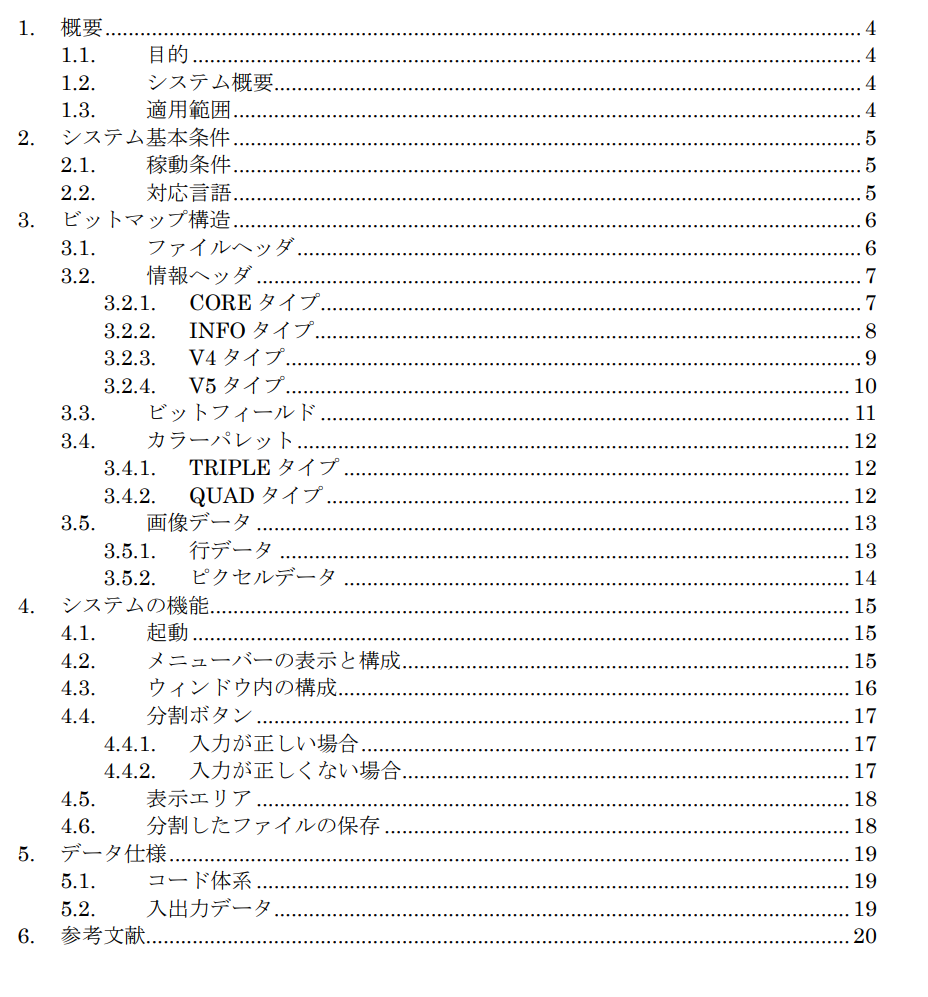
\includegraphics[width=0.95\textwidth]{images/システム仕様書章立ての例.png}
  }
  \captionof{figure}{BMP画像分割アプリのシステム仕様書の章立ての例}
  \label{fig:outline_example}
\end{figure}

\subsection{一般的な章立ての構成要素}
\label{subsec:general_outline}

システム仕様書の章立ては、対象とするシステムの特性や組織の標準により異なるが、システム仕様書として作成される文書には、システムが提供する機能や振る舞いを網羅的に記述することが求められる。
国際的な標準としては、IEEE830 (Recommended Practice for Software Requirements Specifications)\cite{ieee830} が広く知られており、機能要件、外部インターフェース、パフォーマンスなどの非機能要件を記述することが推奨されている。

図\ref{fig:ieee830}に、IEEE830に基づくシステム仕様書の章立てに含むべき項目を示す。

% \begin{enumerate}
%     \item \textbf{システム概要}
%     \begin{itemize}
%         \item システムの目的
%         \item 背景
%         \item 全体像
%     \end{itemize}
%     \item \textbf{機能要件}
%     \begin{itemize}
%         \item システムが提供する機能の一覧
%         \item 各機能の詳細な振る舞い(入力・処理・出力)
%     \end{itemize}
%     \item \textbf{ユーザーインターフェース (UI)}
%     \begin{itemize}
%         \item 画面レイアウト
%         \item 画面遷移図
%         \item 操作フロー
%     \end{itemize}
%     \item \textbf{データ要件}
%     \begin{itemize}
%         \item 扱うデータの定義(ER図やデータディクショナリ)
%     \end{itemize}
%     \item \textbf{外部インターフェース}
%     \begin{itemize}
%         \item 外部システムとの連携仕様
%         \item API定義
%     \end{itemize}
%     \item \textbf{非機能要件}
%     \begin{itemize}
%         \item セキュリティ
%         \item 性能
%         \item 信頼性
%         \item 制約事項
%     \end{itemize}
% \end{enumerate}


\begin{figure}[tp]
\begin{tcolorbox}[
  colback=white,
  colframe=black,
  fonttitle=\bfseries,
]
\footnotesize
\ttfamily
\fontsize{10}{11}\selectfont
\begin{verbatim}
1. はじめに
   1.1 本書の目的
   1.2 対象範囲
   1.3 用語定義・略語
   1.4 参考資料
   1.5 本書の構成

2. システム概要
   2.1 システムの全体像
    2.1.1 システム間インターフェース
    2.1.2 画面インターフェース
    2.1.3 ハードウェア構成
    2.1.4 ソフトウェア構成
    2.1.5 ネットワーク構成
    2.1.6 リソース制約
    2.1.7 運用環境
    2.1.8 設置条件
   2.2 システムの主な機能
   2.3 想定利用者
   2.4 制約事項
   2.5 前提条件および依存関係
   2.6 将来対応事項

3. 詳細要件
   3.1 外部インターフェース仕様
   3.2 機能要件
   3.3 性能要件
   3.4 データベース要件
   3.5 設計上の制約事項
   3.6 システム品質特性
    3.6.1 信頼性
    3.6.2 可用性
    3.6.3 セキュリティ
    3.6.4 保守性
    3.6.5 移植性
   3.7 その他の要件

4. 参考資料
   4.1 索引
   4.2 付録
\end{verbatim}
\end{tcolorbox}
\par\vspace{-20pt}
\captionof{figure}{IEEE830に基づくシステム仕様書の章立てに含むべき項目}
\label{fig:ieee830}
\end{figure}


% \begin{enumerate}
%     \item \textbf{はじめに}
%     \begin{enumerate}[label=1.\arabic*]
%         \item 本書の目的
%         \item 対象範囲
%         \item 用語定義・略語
%         % \item 参考資料
%         \item 本書の構成
%     \end{enumerate}

%     \item \textbf{システム概要}
%     \begin{enumerate}[label=2.\arabic*]
%         \item システムの全体像
%         \begin{enumerate}[label=2.1.\arabic*]
%             \item システム間インターフェース
%             \item 画面インターフェース
%             \item ハードウェア構成
%             \item ソフトウェア構成
%             \item ネットワーク構成
%             \item リソース制約
%             \item 運用環境
%             \item 設置条件
%         \end{enumerate}
%         \item システムの主な機能
%         \item 想定利用者
%         \item 制約事項
%         \item 前提条件および依存関係
%         \item 将来対応事項
%     \end{enumerate}

%     \item \textbf{詳細要件}
%     \begin{enumerate}[label=3.\arabic*]
%         \item 外部インターフェース仕様
%         \item 機能要件
%         \item 性能要件
%         \item データベース要件
%         \item 設計上の制約事項
%         \item システム品質特性
%         \begin{enumerate}[label=3.6.\arabic*]
%             \item 信頼性
%             \item 可用性
%             \item セキュリティ
%             \item 保守性
%             \item 移植性
%         \end{enumerate}
%         \item その他の要件
%     \end{enumerate}

%     \item \textbf{参考資料}
%     \begin{enumerate}[label=4.\arabic*]
%         \item 索引
%         \item 付録
%     \end{enumerate}
% \end{enumerate}


本研究で対象とするシステム仕様書の章立ては、標準的な構成要素を踏まえつつ、対象システム特有の要件を反映した、章、節、項も含めた構成を目指す。


\section{Large Language Models (LLM)}
\label{sec:llm}

Large Language Models (大規模言語モデル)\cite{whatllm}は、膨大なテキストデータと高度なディープラーニング技術を用いて構築された、自然言語処理分野における技術である。

本研究では、OpenAI\cite{openai}社が提供するLLMであるGPT-5.2\cite{gpt52}を搭載したChatGPT\cite{chatgpt}を、システム仕様書章立ての生成に用いる。

\section{プロンプトエンジニアリング}
\label{sec:prompt_engineering}

プロンプトエンジニアリングとは、LLMにタスクの実行を命令する際、LLMから望ましい出力を得るために、入力するプロンプトを設計、および最適化する技術のことである\cite{prompt_engineering}。
LLMの性能を最大限に引き出すためには、モデルの特性を理解して、適切なプロンプトを構築し、入力する必要がある。以降、本研究で用いるプロンプトエンジニアリングに関連する主要な手法について述べる。

\subsection{Few-shot Prompting}
\label{subsec:few_shot}

Few-shot Prompting\cite{fewshot}は、いくつかの入力例と出力例のペアを提示することで、LLMにタスクの意図を理解させて、望ましい形式や内容で出力を生成できるよう誘導する手法である。
図\ref{fig:few}に、Few-shot Promptingの具体例を示す。

図\ref{fig:few}のプロンプト例における、入力例は、「フランスの首都」、「日本の首都」、「アメリカの首都」、「イギリスの首都」であり、出力例は、「パリ」、「東京」、「ワシントンD.C」、「ロンドン」である。

\begin{figure}[tp]
\begin{tcolorbox}[
  colback=white,
  colframe=blue,
  fonttitle=\bfseries,
]
\footnotesize
\ttfamily
\fontsize{10}{11}\selectfont
\begin{verbatim}
フランスの首都：パリ
日本の首都：東京
アメリカの首都：ワシントンD.C.
イギリスの首都：ロンドン
では、ブラジルの首都は？
\end{verbatim}
\end{tcolorbox}
% \par\vspace{-20pt}
\captionof{figure}{Few-shot Promptingの例}
\label{fig:few}
\end{figure}

% \begin{table}[tp]
%   \caption{図\ref{fig:few}における入力例と出力例}
%   \label{tb:inoutexample}
%   \centering
%   \begin{tabular}{|c|c|}
%     \hline
%     \textbf{入力例} & \textbf{出力例} \\
%     \hline\hline
%     フランスの首都 & パリ \\
%     \hline
%     日本の首都 & 東京 \\
%     \hline
%     アメリカの首都 & ワシントンD.C. \\
%     \hline
%     イギリスの首都 & ロンドン \\
%     \hline
%   \end{tabular}
% \end{table}


\subsection{One-shot Prompting}
\label{subsec:one_shot}

One-shot Prompting\cite{oneshot}は、1つの入力例と出力例のペアを提示することで、LLMにタスクの意図を理解させて、望ましい形式や内容で出力を生成できるよう誘導する手法である。
図\ref{fig:one}に、One-shot Promptingの具体例を示す。この例では、「日本の首都」が入力例、「東京」が出力例となる。

\begin{figure}[tp]
\begin{tcolorbox}[
  colback=white,
  colframe=blue,
  fonttitle=\bfseries,
]
\footnotesize
\ttfamily
\fontsize{10}{11}\selectfont
\begin{verbatim}
日本の首都：東京。
では、ブラジルの首都は？
\end{verbatim}
\end{tcolorbox}
\captionof{figure}{One-shot Promptingの例}
\label{fig:one}
\end{figure}

\subsection{Zero-shot Prompting}
\label{subsec:zero_shot}

Zero-shot Prompting\cite{zeroshot}は、LLMに対してタスクの具体的な回答例を与えずに、指示のみでタスクを実行させる手法である。
図\ref{fig:zero}に、Zero-shot Promptingの具体例を示す。


\begin{figure}[tp]
\begin{tcolorbox}[
  colback=white,
  colframe=blue,
  fonttitle=\bfseries,
]
\footnotesize
\ttfamily
\fontsize{10}{11}\selectfont
\begin{verbatim}
ブラジルの首都は？
\end{verbatim}
\end{tcolorbox}
% \par\vspace{-20pt}
% \captionof{figure}{プロンプトの"役割付与"部分}
\captionof{figure}{Zero-shot Promptingの例}
\label{fig:zero}
\end{figure}



Tom Brownらの研究によると、Few-shot PromptingとOne-shot Promptingは、Zero-shot Promptingと比較して、出力の精度が高いとされる\cite{zeroonefew}。一方で、入力例と出力例のペアの作成が困難な場合は、Zero-shot Promptingが用いられる。

本研究でLLMの生成の対象としている章立ては、正解がなく、入力例と出力例を作成することが困難である。
そのため、本研究で提案するシステム仕様書章立て生成プロンプトは、Zero-shot Promptingの手法をベースとする。
ただし、LLMが生成する章立てが意図する章立ての構造とかけ離れたものにならないように、出力例として実際の開発現場で用いられている章立てのテンプレートをLLMに与える(詳細は第\ref{cha:Proposal}章で後述)。
したがって、本研究で提案するシステム仕様書章立て生成プロンプトは、具体的な入力例は与えないが、出力例は与えるため、One-shot Promptingを部分的に取り入れたプロンプトになっていると言える。

\section{プロンプトパターン}
\label{sec:prompt_patterns}

プロンプトパターンとは、特定の状況で課題解決に有効なプロンプトのパターンのことである\cite{nishino}。

本研究で提案するシステム仕様書章立て生成プロンプトでは、Jules Whiteらが提案するプロンプトパターンカタログ\cite{prompt-patterns}を参考に、以下の3つパターンを適用する。

\subsection{Persona Pattern}
\label{subsec:persona_pattern}

Persona Pattern (ペルソナパターン)は、LLMに対して特定の役割(ペルソナ)を与えることで、その役割に適した振る舞いや回答を促すパターンである\cite{prompt-patterns}。
Aobo Kongらの研究により、LLMに適切な役割を与えることで、回答の精度が向上することが示されている\cite{role_assignment}。

本研究で提案するシステム仕様書章立て生成プロンプトでは、文頭で「あなたはシステム仕様書作成の専門アシスタントです」と役割を与えることで、専門的かつ実務的な章立ての出力を誘導する(詳細は第\ref{cha:Proposal}章で後述)。

\subsection{Template Pattern}
\label{subsec:template_pattern}

Template Pattern (テンプレートパターン)は、LLMに対して出力の形式を具体的かつ厳密に指定するパターンである\cite{prompt-patterns}。

本研究で提案するシステム仕様書章立て生成プロンプトでは、マークダウンの番号付きリストを出力形式として強制することで、可読性の高い出力を目指す(詳細は第\ref{cha:Proposal}章で後述)。

\subsection{Context Manager Pattern}
\label{subsec:context_manager_pattern}

Context Manager Pattern (コンテキストマネージャパターン)は、LLMに対して考慮すべき情報の範囲を明示的に指定、あるいは除外することで、回答内容の焦点や関連性を制御するパターンである\cite{prompt-patterns}。
LLMが、タスクの実行時に対話の履歴や曖昧な指示に含まれる無関係な情報に影響され、意図しない回答を生成する場合があるために、このパターンを適用する。

本パターンは、以下の指示を与えることで、LLMの出力を制御することを目的とする。

\begin{itemize}
    \item \textbf{範囲の指定}: 特定のトピックや条件下でのみ回答するように制限する。
    \item \textbf{考慮事項の指定}: 重要な概念や事実を明示し、それに基づいた回答を促す。
    \item \textbf{除外事項の指定}: フォーマットや特定のトピックなど、考慮すべきでない要素を回答から排除する。
\end{itemize}

本研究で提案するシステム仕様書章立て生成プロンプトでは、対象とするシステムの情報(考慮事項)を与えたり、記述すべきでない事項(除外事項)や記述の範囲を厳密に定義したりするために、このパターンを利用する(詳細は第\ref{cha:Proposal}章で後述)。

\iffalse
\clearpage
\begin{figure}[H]
  \centering
  % \fbox{
  \includegraphics[width=0.95\textwidth]{images/vmodel.pdf}
  % }
  \captionof{figure}{システム開発の流れ}
  \label{fig:system_development_process}
\end{figure}

\section{システム仕様書}
\label{sec:system_spec}

\subsection{本研究におけるシステム仕様書の位置づけ}
\label{subsec:system_spec_position}
% 図\ref{fig:system_development_process}に、一般的なシステム開発の流れと本研究でモデルケースとする株式会社スカイコム\cite{skycom}のシステム開発の流れを示す。
% 一般に、システム開発では、顧客の要望をまとめた要件定義書の作成から始まり、設計、実装へと進むプロセスが標準的である\cite{sisutemukaihatu}。
% 一方、本研究でモデルケースとする株式会社スカイコム\cite{skycom}のシステム開発プロセスにおいては、要件定義書は作成せず、システム仕様書がシステム開発における最初の成果物となる。
本研究でモデルケースとする株式会社スカイコム\cite{skycom}のシステム開発の流れを図\ref{fig:system_development_process}に示す。

本研究におけるシステム仕様書は、顧客の要望や口頭での指示といった曖昧な情報を初めて具体的な要件および設計情報として文書化する役割を担い、システム開発における最初の成果物として位置付けている。

% これを踏まえ、本研究では以下の2段階のドキュメント構成を前提とする。

% \begin{enumerate}
%   \item \textbf{システム仕様書(本研究の対象)}: 
%   開発の起点となる文書。顧客の要望(定性的な要件)を整理し、それをシステムとして「何を作るべきか」という具体的な外部仕様に落とし込んだもの。一般的な要件定義書と基本設計書(外部設計書)\cite{kihonsyousaisekkei}の役割を兼ねる。
%   \item \textbf{プログラム設計書}: 
%   システム仕様書を実現するために、具体的に「どう作るか」を記述した文書。使用するクラス、メソッド、処理手順などの内部構造が含まれる。
% \end{enumerate}

% すなわち、本研究におけるシステム仕様書は、要件定義を含内包した基本設計書に相当する。
% このドキュメントは、以下の2つの目的を達成するために作成する。

\begin{itemize}
  \item \textbf{実装者(プログラマ)への指針}:
  システム開発の経験の少ない新人プログラマであっても、仕様書を読むことでシステムの挙動を正しく理解し、迷いなく設計・実装に着手できること。
  \item \textbf{テスト担当者への基準}:
  システムの内部構造(コード)を知らないテスト担当者が、仕様書に記載された正常系・異常系の条件に従って、ブラックボックステストの項目を作成できること。
\end{itemize}

したがって、システム仕様書の記述スタイルとしては、新人プログラマであっても仕様書を理解できるように、専門用語や初出単語の丁寧な説明が求められ、特にシステムの概要や振る舞いについては、テキストだけでなく図(ユースケース図や簡易図)を用いて視覚的に説明することが不可欠である。
また、記述の粒度としては、画面レイアウトや操作フローといった「外部仕様(ユーザーから見える振る舞い)」に焦点を当て、データ型や制約条件は網羅するものの、クラス図や具体的なアルゴリズムといった「内部仕様」は含まないこととする。

\clearpage
\begin{figure}[H]
  \centering
  % \fbox{
  \includegraphics[width=0.95\textwidth]{images/vmodel.pdf}
  % }
  \captionof{figure}{本研究で用いる章立てテンプレート}
  \label{fig:system_development_process}
\end{figure}

\subsection{システム仕様書の章立て}
\label{subsec:general_spec}

システム仕様書の章立ては、プロジェクトの特性や組織の標準により異なるが、システム仕様書として作成される文書には、システムが提供する機能や振る舞いを網羅的に記述することが求められる。
国際的な標準としては、IEEE 830 (Recommended Practice for Software Requirements Specifications)\cite{ieee830} が広く知られており、機能要件、外部インターフェース、パフォーマンスなどの非機能要件を記述することが推奨されている。

これらを踏まえ、一般的なシステム仕様書の章立ては、主に以下の要素で構成することが多い。
% これらを踏まえ、システム仕様書の章立てには、主に以下の要素を含むことが望まれる。

\begin{enumerate}
    \item \textbf{はじめに}
    \begin{enumerate}[label=1.\arabic*]
        \item 本書の目的
        \item 対象範囲
        \item 用語定義・略語
        \item 参考資料
        \item 本書の構成
    \end{enumerate}

    \item \textbf{システム概要}
    \begin{enumerate}[label=2.\arabic*]
        \item システムの全体像
        \begin{enumerate}[label=2.1.\arabic*]
            \item システム間インターフェース
            \item 画面インターフェース
            \item ハードウェア構成
            \item ソフトウェア構成
            \item ネットワーク構成
            \item リソース制約
            \item 運用環境
            \item 設置条件
        \end{enumerate}
        \item システムの主な機能
        \item 想定利用者
        \item 制約事項
        \item 前提条件および依存関係
        \item 将来対応事項
    \end{enumerate}

    \item \textbf{詳細要件}
    \begin{enumerate}[label=3.\arabic*]
        \item 外部インターフェース仕様
        \item 機能要件
        \item 性能要件
        \item データベース要件
        \item 設計上の制約事項
        \item システム品質特性
        \begin{enumerate}[label=3.6.\arabic*]
            \item 信頼性
            \item 可用性
            \item セキュリティ
            \item 保守性
            \item 移植性
        \end{enumerate}
        \item その他の要件
    \end{enumerate}

    \item \textbf{参考資料}
    \begin{enumerate}[label=4.\arabic*]
        \item 索引
        \item 付録
    \end{enumerate}
\end{enumerate}

本研究で対象とするシステム仕様書も、これらの標準的な構成要素を網羅しつつ、実装者が迷わずに開発を行える粒度での記述を目指している。
% 以下に、本研究で対象とするシステム仕様書の章立てテンプレートを示し、各章で記述すべき内容について具体例を交えて説明する。

\fi

% \subsubsection{1. 概要}
% 本章では、システム開発の目的、システムの全体像、および仕様書が適用される範囲を記述する。
% \begin{itemize}
%   \item \textbf{1.1 目的}: なぜこのシステムを開発するのか、解決すべき課題や達成すべき目標を記述する。\\
%   (例: 「本システムは、従来の手作業による在庫管理の非効率性を解消し、リアルタイムでの在庫状況把握を可能にすることを目的とする。」)
%   \item \textbf{1.2 システム概要}: システムが提供する主な機能や特徴を概説する。\\
%   (例: 「本システムは、Webブラウザからアクセス可能な在庫管理システムであり、入出庫登録、在庫照会、棚卸し支援の3つの主要機能を提供する。」)
%   \item \textbf{1.3 適用範囲}: 本仕様書が対象とするシステムの範囲、および対象外とする範囲を明確にする。\\
%   (例: 「本仕様書は在庫管理機能を対象とし、会計システムとの連携インターフェースは別途定義する。」)
% \end{itemize}

% \subsubsection{2. システム基本条件}
% 本章では、システムが稼働するための前提条件や制約事項を記述する。
% \begin{itemize}
%   \item \textbf{2.1 稼働条件}: システムが正常に動作するために必要な条件を記述する。\\
%   (例: 「本システムは24時間365日稼働を前提とし、計画停止は月1回、深夜2時から4時の間に実施する。」)
%   \item \textbf{2.2 他システムインターフェース}: 連携する外部システムとのインターフェース仕様を記述する。\\
%   (例: 「会計システムとはCSV形式のファイル連携を行い、毎日23時に売上データを出力する。」)
%   \item \textbf{2.3 性能条件}: 応答時間、処理能力などの性能要件を記述する。\\
%   (例: 「画面レスポンスは3秒以内、同時接続ユーザー数は最大100名を想定する。」)
%   \item \textbf{2.4 拡張条件}: 将来的な機能拡張や規模拡大に関する条件を記述する。\\
%   (例: 「取扱商品数は現在1万件だが、5年後に5万件への拡張を想定する。」)
%   \item \textbf{2.5 継承条件}: 既存システムから引き継ぐデータや機能を記述する。\\
%   (例: 「現行Excelで管理している商品マスタ(約8,000件)を新システムに移行する。」)
%   \item \textbf{2.6 移行環境}: システム移行時の環境や方法を記述する。\\
%   (例: 「移行は週末2日間で実施し、並行稼働期間を1週間設ける。」)
% \end{itemize}

% \subsubsection{3. システム構成}
% 本章では、システムを構成するハードウェア、ネットワーク、ソフトウェアの構成を記述する。
% \begin{itemize}
%   \item \textbf{3.1 ハードウェア構成及びネットワーク構成}: サーバー、クライアント、ネットワーク機器の構成を図示し説明する。\\
%   (例: 「Webサーバー1台、DBサーバー1台をクラウド環境(AWS)上に構築し、社内LANからVPN経由でアクセスする。」)
%   \item \textbf{3.2 ソフトウェア構成}: 使用するOS、ミドルウェア、フレームワーク等を記述する。\\
%   (例: 「OS: Ubuntu 22.04 LTS、Webサーバー: Nginx、DB: PostgreSQL 15、アプリケーション: Python 3.11 + Django 4.2」)
% \end{itemize}

% \subsubsection{4. システムの機能}
% 本章では、システムが提供する機能の全体像と個々の機能の詳細を記述する。
% \begin{itemize}
%   \item \textbf{4.1 機能構成}: システム全体の機能構成を階層的に示す。\\
%   (例: 機能一覧表や機能構成図を用いて、「在庫管理」「マスタ管理」「帳票出力」などの大機能と、それぞれに含まれる中機能・小機能を記述する。)
%   \item \textbf{4.2 個別機能概要}: 各機能について、入力・処理・出力の観点から詳細を記述する。\\
%   (例: 「入出庫登録機能: 商品コードと数量を入力し、在庫数を更新する。入力値の妥当性チェック後、在庫テーブルを更新し、処理結果を画面に表示する。」)
% \end{itemize}

% \subsubsection{5. システムの運用}
% 本章では、システムの日常的な運用方法や障害時の対応を記述する。
% \begin{itemize}
%   \item \textbf{5.1 運用方法}: 日常の運用体制、監視方法、バックアップ方針などを記述する。\\
%   (例: 「システム監視は運用チームが平日9時〜18時に実施し、夜間・休日はアラート監視とする。」)
%   \item \textbf{5.2 各業務(機能)の運用}: 個々の業務や機能に関する運用手順を記述する。\\
%   (例: 「月次棚卸し処理は毎月末日の業務終了後に実行し、棚卸しレポートを翌営業日に配布する。」)
%   \item \textbf{5.3 障害時の運用}: 障害発生時の対応手順、復旧方法を記述する。\\
%   (例: 「DBサーバー障害時は、直近のバックアップからリストアを行い、最大1時間以内の復旧を目標とする。」)
% \end{itemize}

% \subsubsection{6. セキュリティ}
% 本章では、システムのセキュリティ要件と対策を記述する。\\
% (例: 「ユーザー認証はID/パスワード方式とし、パスワードは8文字以上で英数字混合を必須とする。通信はHTTPS(TLS 1.3)で暗号化する。アクセスログは1年間保持する。」)

% \subsubsection{7. 安全設計}
% 本章では、システムの信頼性・可用性を確保するための設計方針を記述する。\\
% (例: 「重要データの更新処理はトランザクション管理を行い、異常終了時はロールバックする。DBは日次でフルバックアップ、差分バックアップは4時間ごとに取得する。」)

% \subsubsection{8. データ仕様}
% 本章では、システムで扱うデータの詳細仕様を記述する。
% \begin{itemize}
%   \item \textbf{8.1 コード体系}: システムで使用するコードの体系と採番ルールを記述する。\\
%   (例: 「商品コードは10桁の英数字とし、先頭2桁はカテゴリ、次の3桁はサブカテゴリ、残り5桁は連番とする。」)
%   \item \textbf{8.2 データベース}: テーブル定義、ER図、インデックス設計などを記述する。\\
%   (例: 主要テーブルの一覧とカラム定義、テーブル間のリレーションを示すER図を記載する。)
%   \item \textbf{8.3 ファイル}: システムで使用するファイルの形式、レイアウトを記述する。\\
%   (例: 「会計連携用CSVファイルは、文字コードUTF-8、カンマ区切り、先頭行にヘッダーを含む。」)
%   \item \textbf{8.4 入出力データ}: 画面や帳票の入出力データ項目を記述する。\\
%   (例: 画面項目一覧として、項目名、データ型、桁数、必須/任意、入力チェック仕様を記載する。)
%   \item \textbf{8.5 メッセージ}: システムが出力するメッセージの一覧と内容を記述する。\\
%   (例: 「エラーコードE001: "商品コードが未入力です。"」のように、メッセージID、メッセージ内容、表示条件を記載する。)
% \end{itemize}

% \subsubsection{9. 付帯事項}
% 本章では、上記の各章に分類されないその他の重要事項を記述する。\\
% (例: 開発スケジュールの概要、前提条件、制約事項、用語集、参考資料一覧など。)



\iffalse
本章では、LaTeX での論文執筆に必要な基本的な書き方について説明する。
LaTeX の詳細な文法については、文献\cite{kimura-latex}に詳しい解説がある。

% \section{セクションとサブセクション}

\verb|\section{}| でセクション、\verb|\subsection{}| でサブセクションを作成できる。

% \subsection{サブセクションの例}

このようにサブセクションを作成できる。
さらに細かく分けたい場合は \verb|\subsubsection{}| も使用できる。

% \section{箇条書き}

% \subsection{番号なし箇条書き}

\verb|itemize| 環境を使用する：

\begin{itemize}
  \item 項目1
  \item 項目2
  \item 項目3
\end{itemize}

% \subsection{番号付き箇条書き}

\verb|enumerate| 環境を使用する：

\begin{enumerate}
  \item 最初の項目 \label{enum:first}
  \item 2番目の項目
    \begin{enumerate}
      \item サブ項目A \label{enum:sub-a}
      \item サブ項目B \label{enum:sub-b}
    \end{enumerate}
  \item 3番目の項目 \label{enum:third}
\end{enumerate}

% \section{強調表示}
リスト項目にもラベルを付けて参照できる。
例えば、\verb|\ref{enum:first}| で\ref{enum:first}を参照でき、
サブ項目は\verb|\ref{enum:sub-a}| で\ref{enum:sub-a}のように参照できる。
\verb|\cref| を使えば、\cref{enum:first}や\cref{enum:sub-a}のように参照できる。

\section{強調表示}

以下のようなフォントスタイルが使用できる：

\begin{itemize}
  \item \textbf{太字}: \verb|\textbf{太字}|
  \item \textit{Italic}: \verb|\textit{Italic}|
  \item \underline{下線}: \verb|\underline{下線}|
\end{itemize}

一部のフォントスタイルは、日本語に対応していないもの (\verb|\textit{斜体}| など) があるので注意。

% \section{verbatim 環境}

コマンドやコードをそのまま表示したい場合は、\verb|verbatim| 環境またはインライン \verb|\verb| コマンドを使用する。

\begin{verbatim}
これは verbatim 環境の例です。
LaTeX のコマンドも \command{そのまま} 表示されます。
\end{verbatim}

インラインで表示する場合は、\verb|\verb|コマンド| のように書く。

% \section{ラベルと参照}

% \subsection{ラベルの付け方}

章、節、図、表などにラベルを付けることで、後から参照できる：

\begin{verbatim}
\section{セクション名}\label{sec:label_name}
\end{verbatim}

% \subsection{参照の仕方}

ラベルを付けた箇所を参照するには、\verb|\ref{}| コマンドを使用する。
例えば、この章は第\ref{cha:Preparation}章であり、第\ref{cha:Introduction}章で本テンプレートの概要を説明した。
\fi

% 提案手法
\chapter{システム仕様書章立て生成プロンプト}\label{cha:Proposal}

本章では、本研究で提案するシステム仕様書章立て生成プロンプトについて述べる。

\section{プロンプトの利用手順}
\label{sec:process}

提案するシステム仕様書章立て生成プロンプトの利用手順は、以下の2ステップである。
また、提案するシステム仕様書章立て生成プロンプトの構成を、図\ref{fig:prompt_structure}に示す。
以降、提案するシステム仕様書章立て生成プロンプトを「提案プロンプト」とする。

\begin{figure}[tp]
  \centering
  \includegraphics[width=0.9\linewidth]{images/prompt_figure.pdf}
  \caption{提案プロンプトの構成}
  \label{fig:prompt_structure}
\end{figure}

\begin{enumerate}
    \item \textbf{システム情報の入力}:
    ユーザー(仕様書作成者)は、図\ref{fig:prompt_structure}の「開発するシステム情報」部分に、対象システムのシステム名とシステム概要を記述する。

    \item \textbf{章立ての生成}:
    章立て生成の対象とする「開発するシステム情報」を入力したプロンプトをLLM(GPT-5.2)に入力し、システム仕様書の章立てを生成する。出力結果として、章立て(章・節・項の構造)を得る。
\end{enumerate}


\section{プロンプトの構成}

提案プロンプトの作成には、Jules Whiteらによるプロンプトパターンカタログ\cite{prompt-patterns}を参考にする。
提案プロンプトは、以下の5つの要素で構成する(図\ref{fig:prompt_structure}を参照)。
\begin{itemize}
  \item 役割付与
  \item ベースの章立て  
  \item 開発するシステム情報
  \item システム仕様書の定義
  \item 章立て出力指示
\end{itemize}

提案プロンプトのテンプレートを、図\ref{fig:prompt_full_text}に示す。

\begin{figure}[tp]
\begin{tcolorbox}[
  colback=white,
  colframe=blue,
  fonttitle=\bfseries,
]
\footnotesize
\ttfamily
\fontsize{7}{7}\selectfont
\begin{verbatim}
あなたはシステム仕様書作成の専門アシスタントです。

【ベース章立てテンプレート(参考)】
1. 概要
 1.1.目的
 1.2.システム概要
 1.3.適用範囲
2. システム基本条件
 2.1.稼働条件
 2.2.他システムインターフェース
 2.3.性能条件
 2.4.拡張条件
 2.5.継承条件
 2.6.以降環境
3. システム構成
 3.1.ハードウェア構成及びネットワーク構成
 3.2.ソフトウェア構成
4. システムの機能
 4.1.機能構成
 4.2.個別機能概要
5. システムの運用
 5.1.運用方法
 5.2.各業務(機能)の運用
 5.3.障害時の運用
6.セキュリティ
7.安全設計
8.データ仕様
 8.1.コード体系
 8.2.データベース
 8.3.ファイル
 8.4.入出力データ
 8.5.メッセージ
9.付帯事項

※ベース章立てはあくまで参考です。必要に応じて章の追加・削除・順序変更を行って、漏れなく体系的な章立てを作成してください。

【開発するシステム情報】
- システム名：
- 概要：

【システム仕様書の定義】
- 目的：
 ・プログラム作成者がシステムの仕様を理解し、設計・実装するための文書 
 ・システムテスト担当者がテスト項目を作るために参照する文書
- 対象読者:
 ・プログラム作成者：新人想定 
 ・テスト担当者：内部構造は知らず、仕様書に記載されたエラー条件に従ってテストを実施
- 記述スタイル：
 ・専門用語は必ず説明 
 ・初出の単語は必ず説明 
 ・システム概要は図を使って視覚的に理解できるようにする 
 ・図はユースケース図または独自の簡易図を使用し、必ずテキストで補足説明 
 ・用語や機能名は文書内で統一 
 ・データ型や制約が必要な場合は表形式で記載 
 ・外部仕様のみ記載(内部構造は書かない)
- システム要件：
 ・動作環境：OS、ハードウェア、ネットワーク 
 ・非機能要件：パフォーマンス、セキュリティ 
- 記述の粒度：
 ・画面レイアウトと操作フローのみ含める

【出力指示】
・上記情報に基づき、開発するシステムのシステム仕様書に必要な章立てを出力してください。
・ここでいう章立ては、以下の内容を含みます。
　・章と節、章タイトル、節タイトル、項、項タイトル 
・出力形式は**マークダウンの番号付きリスト**としてください。 
・章名以外(目的・記述のポイントなど)は一切書かないでください。 
・章の追加や削除、順序の変更は自由に行って構いません。
・人間が考慮し忘れるような章立ても考えるのがあなたの役目です。考慮漏れが無いように、網羅性を高めてください。
\end{verbatim}
\end{tcolorbox}
\par\vspace{-20pt}
\captionof{figure}{提案プロンプトのテンプレート}
\label{fig:prompt_full_text}
\end{figure}

% \subsection{プロンプト構成要素}

% 本節では、提案プロンプトを構成する5つの要素について説明する。
以降、提案プロンプトを構成する5つの要素について説明する。
表\ref{tb:prompt_elements_summary}に、各要素の役割と関連するプロンプトエンジニアリング技術(\ref{sec:prompt_engineering}節を参照)の対応を示す。

\begin{table}[tp]
  \caption{提案プロンプト構成要素と対応する技術と目的}
  \label{tb:prompt_elements_summary}
  \centering
  \small
  \begin{tabular}{|l|p{8cm}|l|} % 幅を調整
    \hline
    \textbf{構成要素} & \textbf{目的と解決する課題} & \textbf{関連技術} \\
    \hline
    役割付与 & 専門的な文体と観点の固定 & Persona Pattern \\
    \hline
    ベースの章立て & 構造の欠落防止、標準的な形式の担保 & One-shot Prompting \\
    \hline
    開発するシステム情報 & 生成内容の具体化 & Context Manager Pattern \\
    \hline
    仕様書の定義 & 記述粒度の制御、不必要な内部情報の排除 & Context Manager Pattern \\
    \hline
    章立て出力指示 & 論理的整合性の確保、出力結果の視認性の確保 & Template Pattern \\
    \hline
  \end{tabular}
\end{table}

\subsubsection{役割付与}

図\ref{fig:prompt_full_text}における「役割付与」部分のプロンプトを、図\ref{fig:role_assignment}に示す。

\begin{figure}[tp]
\vspace{9mm}
\begin{tcolorbox}[
  colback=white,
  colframe=blue,
  fonttitle=\bfseries,
]
\footnotesize
\ttfamily
\fontsize{10}{11}\selectfont
\begin{verbatim}
あなたはシステム仕様書作成の専門アシスタントです。
\end{verbatim}
\end{tcolorbox}
% \par\vspace{-20pt}
\captionof{figure}{「役割付与」部分のプロンプト}
\label{fig:role_assignment}
\end{figure}

プロンプトの文頭で「あなたはシステム仕様書作成の専門アシスタントです」と書くことで、LLMに特定の役割を与える。
これは、\ref{subsec:persona_pattern}節で述べたPersona Pattern(ペルソナパターン)の適用である。
提案プロンプトでは、「システム仕様書作成の専門アシスタント」という役割をLLMに与えることで、LLMの出力をシステム仕様書作成に適したものにする。

\subsubsection{ベースの章立て}

図\ref{fig:prompt_full_text}における「ベースの章立て」部分のプロンプトを、図\ref{fig:base_outline}に示す。
実際の開発現場で使用されている章立てのテンプレートを「ベース章立てテンプレート」として提示する。
これは、\ref{subsec:one_shot}節で述べたOne-shot Promptingの技術を用いて、出力する章立て構造の例示を行っている。



\begin{figure}[tp]
\begin{tcolorbox}[
  colback=white,
  colframe=blue,
  fonttitle=\bfseries,
]
\footnotesize
\ttfamily
\fontsize{9}{10}\selectfont
\begin{verbatim}
【ベース章立てテンプレート(参考)】
1. 概要
 1.1.目的
 1.2.システム概要
 1.3.適用範囲
2. システム基本条件
 2.1.稼働条件
 2.2.他システムインターフェース
 2.3.性能条件
 2.4.拡張条件
 2.5.継承条件
 2.6.以降環境
3. システム構成
 3.1.ハードウェア構成及びネットワーク構成
 3.2.ソフトウェア構成
4. システムの機能
 4.1.機能構成
 4.2.個別機能概要
5. システムの運用
 5.1.運用方法
 5.2.各業務(機能)の運用
 5.3.障害時の運用
6.セキュリティ
7.安全設計
8.データ仕様
 8.1.コード体系
 8.2.データベース
 8.3.ファイル
 8.4.入出力データ
 8.5.メッセージ
9.付帯事項

※ベース章立てはあくまで参考です。必要に応じて章の追加・削除・順序変更を行って、漏れなく体系的な章立てを作成してください。
\end{verbatim}
\end{tcolorbox}
\par\vspace{-20pt}
\captionof{figure}{「ベースの章立て」部分のプロンプト}
\label{fig:base_outline}
\end{figure}


LLMにテンプレートを与えず、ゼロから章立てを生成させると、章の順序が不自然になる、重要な章(例：セキュリティや運用)が抜け落ちるといった「構造的な欠陥」が生じるリスクがある。
そこで、提案プロンプトでは、実際の開発現場で用いられている章立てのテンプレートを初期値(ベース)としてLLMに与えることで、LLMは「何を書くべきか」の探索範囲を絞り込むことができる。
ベースの章立てテンプレートの提示により、章立ての標準的な構成を維持する。

\subsubsection{開発するシステム情報}

 図\ref{fig:prompt_full_text}における「開発するシステム情報」部分のプロンプトテンプレートを、図\ref{fig:development_system_info_template}に示す。
これは、本プロンプトの入力であるシステム名とシステム概要を記述する箇所である。


\begin{figure}[tp]
\begin{tcolorbox}[
  colback=white,
  colframe=blue,
  fonttitle=\bfseries,
]
\footnotesize
\ttfamily
\fontsize{10}{11}\selectfont
\begin{verbatim}
【開発するシステム情報】
- システム名：
- 概要：
\end{verbatim}
\end{tcolorbox}
\par\vspace{-20pt}
\captionof{figure}{「開発するシステム情報」部分のプロンプトテンプレート}
\label{fig:development_system_info_template}
\end{figure}

図\ref{fig:development_system_info}に例として、BMP画像を指定された数に分割し、保存するアプリケーションである、BMP画像分割アプリのシステム情報を入力したプロンプトの例を示す。

\begin{figure}[tp]
\begin{tcolorbox}[
  colback=white,
  colframe=blue,
  fonttitle=\bfseries,
]
\footnotesize
\ttfamily
\fontsize{10}{11}\selectfont
\begin{verbatim}
【開発するシステム情報】
- システム名：BMP画像分割アプリ
- 概要：指定されたBMP画像ファイルを指定された数に分割する。
\end{verbatim}
\end{tcolorbox}
\par\vspace{-20pt}
\captionof{figure}{「開発するシステム情報」を記入したプロンプトの例}
\label{fig:development_system_info}
\end{figure}

また、これは、\ref{subsec:context_manager_pattern}節で述べたContext Manager Patternにおける「考慮事項の指定」に相当する。

対象とするシステム情報をLLMに与えないまま章立てを行わせると、どのシステムにも当てはまるような抽象的な記述を生成するリスクがある。
そこで、提案プロンプトでは、対象システムの具体的なコンテキスト(考慮すべき事実)をLLMに提供することで、LLMがシステム固有の情報に基づいた章立てを出力するように誘導する。
システム情報として、図\ref{fig:development_system_info}に例として示した「BMP画像分割アプリ」に関する入力があることで、LLMに「画像処理に関連する機能要件が必要ではないか？」「ファイル入出力の章が必要ではないか？」といった推論を促す。


\subsubsection{システム仕様書の定義}

図\ref{fig:prompt_full_text}における「システム仕様書の定義」部分のプロンプトを、図\ref{fig:definition_of_system_specification}に示す。
本要素では、システム仕様書がどういう役割の文書であるかをLLMに説明する。
具体的には、以下を定義する。
\begin{itemize}
  \item \textbf{目的}: 仕様書がプロジェクトにおいて果たすべき役割や、作成のねらいを定義する。
  \item \textbf{対象読者}: 仕様書を参照する人物のスキルレベルや立場を指定する。
  \item \textbf{記述スタイル}: 図解の活用や用語の統一など、仕様書としての具体的な表現の指針を規定する。
  \item \textbf{システム要件}: 動作環境や非機能要件で、考慮すべき制約条件を定める。
  \item \textbf{記述の粒度}: 章立てに含める情報の詳細さや、記述を限定する範囲を指定する。
\end{itemize}


\begin{figure}[tp]
\begin{tcolorbox}[
  colback=white,
  colframe=blue,
  fonttitle=\bfseries,
]
\footnotesize
\ttfamily
\fontsize{10}{11}\selectfont
\begin{verbatim}
【システム仕様書の定義】
- 目的：
 ・プログラム作成者がシステムの仕様を理解し、設計・実装するための文書 
 ・システムテスト担当者がテスト項目を作るために参照する文書
- 対象読者:
 ・プログラム作成者：新人想定 
 ・テスト担当者：内部構造は知らず、仕様書に記載されたエラー条件に従ってテストを実施
- 記述スタイル：
 ・専門用語は必ず説明 
 ・初出の単語は必ず説明 
 ・システム概要は図を使って視覚的に理解できるようにする 
 ・図はユースケース図または独自の簡易図を使用し、必ずテキストで補足説明 
 ・用語や機能名は文書内で統一 
 ・データ型や制約が必要な場合は表形式で記載 
 ・外部仕様のみ記載(内部構造は書かない)
- システム要件：
 ・動作環境：OS、ハードウェア、ネットワーク 
 ・非機能要件：パフォーマンス、セキュリティ 
- 記述の粒度：
 ・画面レイアウトと操作フローのみ含める
\end{verbatim}
\end{tcolorbox}
\par\vspace{-20pt}
\captionof{figure}{「システム仕様書の定義」部分のプロンプト}
\label{fig:definition_of_system_specification}
\end{figure}

これは、Context Manager Patternにおける「範囲の指定」および「除外事項の指定」に相当する。

「システム仕様書」という言葉の定義は曖昧であり、要件定義レベルの粗い内容を含む場合や、内部設計レベルの詳細な内容までを含む場合もある\cite{software_engineering}。
したがって、LLMへの指示が曖昧な場合、本研究で想定するシステム仕様書には含むべきでない内部構造の情報を含んでしまったり、逆に含むべき外部仕様の情報を省略したりと、粒度の不一致が発生する。
そこで、提案プロンプトでは、「外部仕様のみ記載する」「内部構造は書かない」と明示的な範囲指定と除外指定をLLMに与えることで、\ref{subsec:system_spec_position}節で定義した本研究におけるシステム仕様書の内容に範囲を限定する。
また、対象読者を新人想定のプログラム作成者とすることで、細部まで明文化した丁寧な記述を促す効果を狙う。さらに、対象読者をシステムテスト担当者とすることで、テスト設計に必要な観点を章立てに反映し、網羅性が向上する効果を狙う。

\subsubsection{章立て出力指示}

図\ref{fig:prompt_full_text}における「出力指示」部分のプロンプトを、図\ref{fig:output_instruction}に示す。
本要素では、システム仕様書の章立てを生成する際のLLMに対する出力指示を行う。
出力指示には、以下の内容を含める。
\begin{itemize}
  \item 章立て生成指示
  \item 章立ての定義
  \item 章立ての出力形式を「マークダウンの番号付きリスト」に制限する指示
  \item 章立てに関係のない内容は出力しないよう促す指示
  \item 自由な章立てを促す指示
  \item 章立ての網羅性を高める指示
\end{itemize}


\begin{figure}[tp]
\begin{tcolorbox}[
  colback=white,
  colframe=blue,
  fonttitle=\bfseries,
]
\footnotesize
\ttfamily
\fontsize{10}{11}\selectfont
\begin{verbatim}
【出力指示】
・上記情報に基づき、開発するシステムのシステム仕様書に必要な章立てを出力してください。
・ここでいう章立ては、以下の内容を含みます。
　・章と節、章タイトル、節タイトル、項、項タイトル 
・出力形式は**マークダウンの番号付きリスト**としてください。 
・章名以外(目的・記述のポイントなど)は一切書かないでください。 
・章の追加や削除、順序の変更は自由に行って構いません。
・人間が考慮し忘れるような章立ても考えるのがあなたの役目です。考慮漏れが無いように、網羅性を高めてください。
\end{verbatim}
\end{tcolorbox}
\par\vspace{-20pt}
\captionof{figure}{「出力指示」部分のプロンプト}
\label{fig:output_instruction}
\end{figure}


章立て生成指示と章立ての定義により、何を出力すべきかをLLMに理解させる。
また、出力形式を「マークダウンの番号付きリスト」に制限する指示と章立てに関係のない内容は出力しないよう促す2つの出力形式指定により、出力結果の視認性を高めることを目的とする。
ここで、「マークダウンの番号付きリスト」に制限する指示は、\ref{subsec:template_pattern}節で述べたTemplate Patternの適用である。
そして、自由な章立てを促す指示と章立ての網羅性を高める指示により、LLMの膨大な学習データを活かし、より網羅性の高い章立てを生成することを目指す。


図\ref{fig:output_instruction}の出力指示におけるLLMの出力例を、図\ref{fig:output_instruction_correct}に示す。
出力形式指定をすることで、LLMは階層化された章立てのみを出力する。
また、図\ref{fig:output_instruction}の出力指示から2つの出力形式指定を削除した出力指示を図\ref{fig:no_format}に、図\ref{fig:no_format}の出力指示におけるLLMの出力例を図\ref{fig:output_instruction_no_format}に、それぞれ示す。

図\ref{fig:output_instruction_no_format}の赤枠で囲んだ部分を見てわかるように、出力形式指定のない出力指示では、LLMは章立てそのものだけでなく、章立てに関係のないものまで出力してしまうことが分かる。
したがって、提案プロンプトでは、出力形式指定をすることで、LLMの出力を構造化し、可読性を向上させ、人間が目視で章立てを確認する際の認知的負荷を軽減できる。



\begin{figure}[tp]
  \centering
  \fbox{
  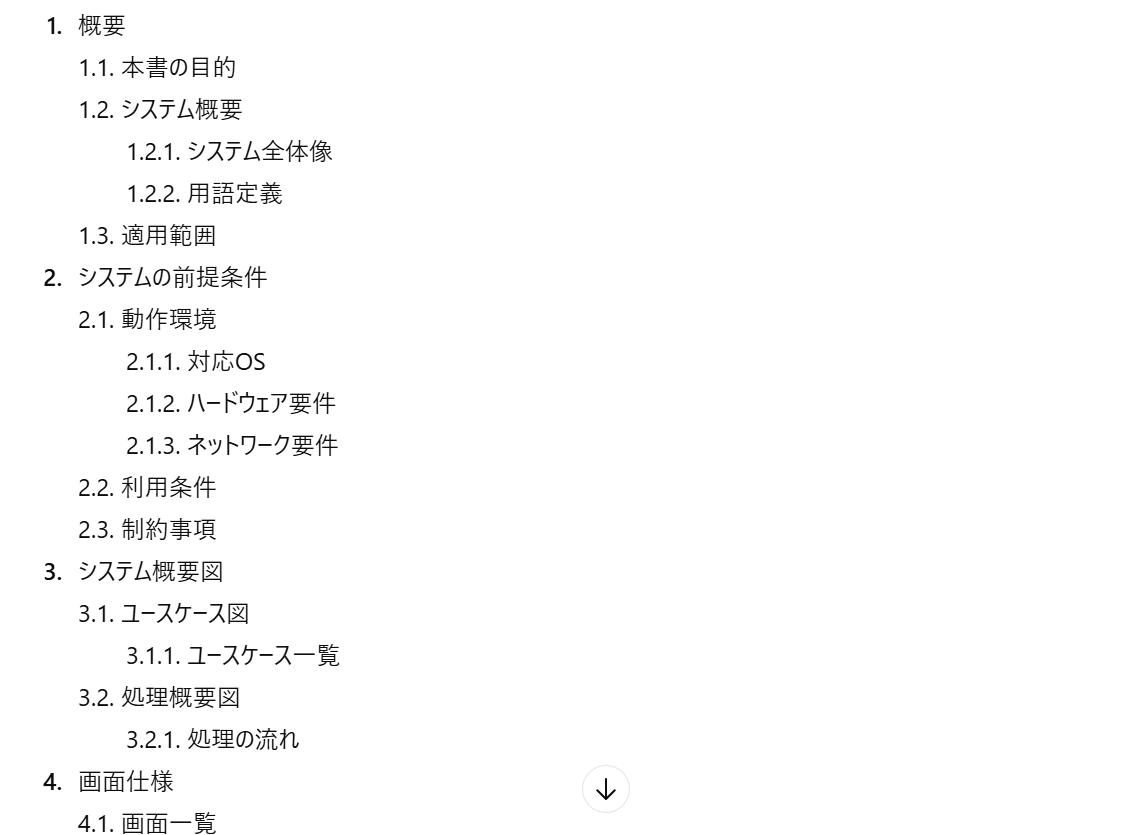
\includegraphics[width=0.8\textwidth]{images/正しい出力.png}
  }
  \captionof{figure}{出力形式指定ありの出力指示での出力例の一部}
  \label{fig:output_instruction_correct}
\end{figure}



\begin{figure}[tp]
\begin{tcolorbox}[
  colback=white,
  colframe=blue,
  fonttitle=\bfseries,
]
\footnotesize
\ttfamily
\fontsize{10}{11}\selectfont
\begin{verbatim}
【出力指示】
・上記情報に基づき、開発するシステムのシステム仕様書に必要な章立てを出力してください。
・ここでいう章立ては、以下の内容を含みます。
　・章と節、章タイトル、節タイトル、項、項タイトル
・章の追加や削除、順序の変更は自由に行って構いません。
・人間が考慮し忘れるような章立ても考えるのがあなたの役目です。考慮漏れが無いように、網羅性を高めてください。
\end{verbatim}
\end{tcolorbox}
\par\vspace{-20pt}
\captionof{figure}{図\ref{fig:output_instruction}から出力形式指定を削除した出力指示}
\label{fig:no_format}
\end{figure}

\begin{figure}[tp]
  \centering
  \fbox{
  \includegraphics[width=0.8\textwidth]{images/出力指示不適切な例.pdf}
  }
  \captionof{figure}{図\ref{fig:no_format}のプロンプトでの出力例の一部}
  \label{fig:output_instruction_no_format}
\end{figure}


\iffalse
本章では、図、表、数式の挿入方法について説明する。

% \section{図の挿入}

図を挿入するには、\verb|figure| 環境と \verb|\includegraphics| コマンドを使用する。

% \subsection{基本的な図の挿入}

図\ref{fig:example}に例を示す。

\begin{figure}[tp]
  \centering
  \includegraphics[width=0.5\linewidth]{./images/syokuji_computer.png}
  \caption{図の挿入例}
  \label{fig:example}
\end{figure}

上記の図は以下のコードで挿入できる：

\begin{verbatim}
\begin{figure}[tp]
  \centering
  \includegraphics[width=0.5\linewidth]{./images/syokuji_computer.png}
  \caption{図の挿入例}
  \label{fig:example}
\end{figure}
\end{verbatim}

% \subsection{画像ファイルの配置}

画像ファイルは \verb|images/| ディレクトリに配置する。
サポートされている画像形式：PNG、JPG、PDF など。

% \section{表の挿入}

表を挿入するには、\verb|table| 環境と \verb|tabular| 環境を使用する。

% \subsection{基本的な表の挿入}

表\ref{tb:example}に例を示す。

\begin{table}[tp]
  \caption{表の挿入例}
  \label{tb:example}
  \centering
  \begin{tabular}{|l|c|r|}
    \hline
    左寄せ & 中央寄せ & 右寄せ \\
    \hline
    データ1 & データ2 & データ3 \\
    データ4 & データ5 & データ6 \\
    \hline
  \end{tabular}
\end{table}

上記の表は以下のコードで挿入できる：

\begin{verbatim}
\begin{table}[tp]
  \caption{表の挿入例}
  \label{tb:example}
  \centering
  \begin{tabular}{|l|c|r|}
    \hline
    左寄せ & 中央寄せ & 右寄せ \\
    \hline
    データ1 & データ2 & データ3 \\
    データ4 & データ5 & データ6 \\
    \hline
  \end{tabular}
\end{table}
\end{verbatim}

% \section{数式の挿入}

% \subsection{インライン数式}

文中に数式を挿入する場合は、\verb|$...$| または \verb|\(...\)| を使用する。
例：$E = mc^2$ は有名な公式である。

% \subsection{ディスプレイ数式}

独立した行に数式を表示する場合は、\verb|equation| 環境を使用する。

\begin{equation}\label{eq:example}
  \int_0^\infty e^{-x^2} dx = \frac{\sqrt{\pi}}{2}
\end{equation}

式(\ref{eq:example})のように、数式にも番号とラベルを付けて参照できる。

% \subsection{複数行の数式}

複数行の数式を表示する場合は、\verb|align| 環境を使用する：

\begin{align}
  a + b &= c \\
  x + y &= z
\end{align}

% \section{図表の参照}

図や表を参照するには、\verb|\ref{}| コマンドを使用する：

\begin{itemize}
  \item 図\ref{fig:example}のように図を参照
  \item 表\ref{tb:example}のように表を参照
  \item 式(\ref{eq:example})のように数式を参照
\end{itemize}
\fi

% 適用例
% \chapter{適用例}\label{cha:Application}


% 本章では、第\ref{cha:Proposal}章で作成したプロンプトを、適用した結果を示す。
% 適用対象として、「授業出席管理システム」を選定した。
% 本事例を通じて、プロンプトへの入力内容、および生成する2段階の出力（章立て構造と詳細説明）の具体像を示す。

% \section{プロンプトへの入力}

% 本プロンプトの「開発するシステム情報」に、システム概要を以下のように入力した。

% \begin{figure}[H]
% \begin{tcolorbox}[colback=white, colframe=black]
% \begin{verbatim}
% システム名: 授業出席管理システム
% 概要: 学生が自身のスマートフォンを用いて授業の出席登録を行い、教員がリアルタイムで出席状況や過去の履歴を管理・集計するシステム。
% \end{verbatim}
% \end{tcolorbox}
% \caption{適用例における開発するシステム情報}
% \label{fig:app_input}
% \end{figure}

% \section{生成結果}

% プロンプトを実行した結果、以下の出力を得た。

% \subsection{章立て（構造）}

% 出力は、章立て構造を示す。
% 画面仕様、操作フロー、機能仕様を見ると、ドメイン独自の章立て構造を生成していることが確認できる。


% \begin{figure}[H]
% \begin{tcolorbox}[
%   colback=white,
%   colframe=black,
%   fonttitle=\bfseries
% ]
% \begin{multicols}{2}
% \footnotesize
% \ttfamily
% \fontsize{11}{12}\selectfont
% \begin{verbatim}
% 1. 概要
%     1.1. 目的
%     1.2. システム概要
%     1.3. 用語定義
%     1.4. 適用範囲

% 2. システム全体像
%     2.1. 利用者区分
%     2.2. ユースケース一覧
%     2.3. システム構成図

% 3. 動作環境・基本条件
%     3.1. 動作環境
%     3.2. ネットワーク条件
%     3.3. 稼働条件
%     3.4. 制約事項

% 4. 画面仕様
%     4.1. 画面一覧
%     4.2. 学生向け画面
%         4.2.1. 出席登録画面
%         4.2.2. 出席履歴確認画面
%     4.3. 教員向け画面
%         4.3.1. 出席状況確認画面
%         4.3.2. 出席履歴管理画面

% 5. 操作フロー
%     5.1. 学生操作フロー
%     5.2. 教員操作フロー
%     5.3. 例外操作フロー

% 6. 機能仕様
%     6.1. 機能一覧
%     6.2. 出席登録機能
%     6.3. 出席状況確認機能
%     6.4. 出席履歴管理・集計機能

% 7. データ仕様
%     7.1. データ項目一覧
%     7.2. データ型・制約
%     7.3. 入出力データ定義

% 8. エラー・メッセージ仕様
%     8.1. エラー一覧
%     8.2. エラーメッセージ定義

% 9. 非機能要件
%     9.1. パフォーマンス要件
%     9.2. セキュリティ要件
%     9.3. 可用性・信頼性要件

% 10. 運用・保守
%     10.1. 通常運用
%     10.2. 障害時運用
%     10.3. データ保全

% 11. テスト観点整理
%     11.1. テスト対象範囲
%     11.2. テスト前提条件

% 12. 付帯事項
%     12.1. 前提条件
%     12.2. 制限事項
%     12.3. 将来拡張の考慮
% \end{verbatim}
% \end{multicols}
% \end{tcolorbox}
% \caption{適用例における出力}
% \label{fig:app_output1}
% \end{figure}

% \section{まとめ}

% 本適用例により、作成したプロンプトが章立てを生成できることが確認できた。

% 評価
% \input{chapters/05-evaluation.tex}
\chapter{評価実験}\label{cha:Evaluation}

本研究で提案するプロンプトの有用性を検証するため、実験を行った。本実験の被験者は、システム仕様書作成経験のない学生4人である。
実験では、実際のシステム開発を想定した題材を用い、提案プロンプトを用いた手法とその他の手法で、被験者が章立てを作成する。作成した章立ての品質を、
株式会社スカイコム\cite{skycom}にて5年以上のシステム仕様書作成経験を持つ専門家5人が評価者となり、評価した。


\section{実験設定}

\subsection{対象システム}
\label{sec:target_system}

実験の題材として、以下の2つのシステムを選定した。
\begin{enumerate}
    \item \textbf{BMP画像分割アプリ}: BMP画像を指定された数に分割し、保存するアプリケーション
    \item \textbf{クラウド型電子契約サービス}: PDF技術を活かした電子契約/ワークフロー、それらに付随する文書管理、およびユーザー管理機能を持つクラウドサービス
\end{enumerate}

BMP画像分割アプリは機能が少ない単純なシステムとして、クラウド型電子契約サービスは機能が多い複雑なシステムとして、実験対象とした。

\subsection{比較手法}

システム仕様書章立ての作成手法として、以下の3パターンを設定した。
\begin{itemize}
    \item \textbf{手法A(手動作成)}: 被験者はLLMを用いず、章立てを作成する。この際、被験者には、対象システムの情報(\ref{sec:target_system}節を参照)と、ベースの章立て(図\ref{fig:base_outline}を参照)を与える。
    \item \textbf{手法B(自由プロンプト)}: 被験者はLLM(GPT-5.2)を使用して、章立てを作成する。この際、被験者には、対象とするシステムの情報(\ref{sec:target_system}節を参照)と、ベースの章立て(図\ref{fig:base_outline}を参照)を与える。ただし、提案プロンプトは与えずに、被験者自身による自由なプロンプトをLLM(GPT-5.2)に与える。
    \item \textbf{手法C(提案プロンプト)}: 被験者はLLM(GPT-5.2)を使用し、提案プロンプトを用いて章立てを作成する。
\end{itemize}

図\ref{fig:bmp}にBMP画像分割アプリを対象とした手法Cで用いるプロンプトの「開発するシステム情報」部分を示す。
\begin{figure}[tp]
\begin{tcolorbox}[
  colback=white,
  colframe=blue,
  fonttitle=\bfseries,
]
\footnotesize
\ttfamily
\fontsize{10}{11}\selectfont
\begin{verbatim}
【開発するシステム情報】
- システム名：BMP画像分割アプリ
- 概要：指定されたBMP画像ファイルを指定された数に分割する。
\end{verbatim}
\end{tcolorbox}
% \par\vspace{-20pt}
\captionof{figure}{BMP画像分割アプリを対象とした手法Cで用いるプロンプトの「開発するシステム情報」部分}
\label{fig:bmp}
\end{figure}

図\ref{fig:cloud}にクラウド型電子契約サービスを対象とした手法Cで用いるプロンプトの「開発するシステム情報」部分を示す。
\begin{figure}[tp]
\begin{tcolorbox}[
  colback=white,
  colframe=blue,
  fonttitle=\bfseries,
]
\footnotesize
\ttfamily
\fontsize{10}{11}\selectfont
\begin{verbatim}
【開発するシステム情報】
- システム名：クラウド型電子契約サービス
- 概要：PDF技術を活かした電子契約/ワークフロー、それらに付随する文書管理、およびユーザー管理機能を持つクラウドサービス
\end{verbatim}
\end{tcolorbox}
% \par\vspace{-20pt}
\captionof{figure}{クラウド型電子契約サービスを対象とした手法Cで用いるプロンプトの「開発するシステム情報」部分}
\label{fig:cloud}
\end{figure}

\subsection{被験者と実験の割り当て}

表\ref{tb:experiment_allocation}に、被験者ごとの対象システムと手法の割り当てを示す。

\begin{table}[tp]
  \caption{被験者ごとの対象システムと手法の割り当て}
  \label{tb:experiment_allocation}
  \centering
  \begin{tabular}{|c|l|l|}
    \hline
    \textbf{被験者} & \textbf{BMP画像分割アプリ} & \textbf{クラウド型電子契約サービス} \\
    \hline\hline
    A & 手法A(手動) & 手法C(提案プロンプト) \\
    \hline
    B & 手法C(提案プロンプト) & 手法A(手動) \\
    \hline
    C & 手法B(自由プロンプト) & 手法C(提案プロンプト) \\
    \hline
    D & 手法C(提案プロンプト) & 手法B(自由プロンプト) \\
    \hline
  \end{tabular}
\end{table}

\subsection{評価方法}
作成した章立ては、株式会社スカイコムにて5年以上のシステム仕様書作成経験を持つ専門家が評価者となり、評価した。
評価は以下の9項目について行い、それぞれ5段階のリッカート尺度\cite{likert}(5:非常に良い, 4:良い, 3:普通, 2:悪い, 1:非常に悪い)で採点した。

\begin{enumerate}
  \item 最低限含むべき章を含んでいるか(網羅性)
  \item 章の順序は適切か(論理性)
  \item 章タイトルは適切か(命名の適切さ)
  \item 章立て全体として理解しやすいか(可読性)
  \item 章の粒度は適切か(粒度の適切さ)
  \item 想定読者に適した章立てか(適合性)
  \item 将来的な拡張に対応しやすい章立てか(拡張性)
  \item 章、節、項の包含関係は適切か(構造的整合性)
  \item 章立てがシステム独自の章立てになっているか(独自性)
\end{enumerate}

また、これら9項目の定量的な評価に加え、各対象システムに対して、評価者から全体的な所感や各手法に対する改善点を自由記述形式のコメントとして収集した。
そのため、すべての章立てに対して個別のコメントが得られているわけではないが、得られたコメントについては\ref{sec:evaluation_results}節で示す。



% \begin{enumerate}
%     \item 最低限含むべき章を含んでいるか(網羅性)
%     \begin{itemize}
%         \item 5: すべて含まれている
%         \item 4: 軽微な不足がある
%         \item 3: 一部重要な章が不足している
%         \item 2: 多くの重要な章が不足している
%         \item 1: 最低限必要な章が1つも含まれていない
%     \end{itemize}
%     \item 章の順序は適切か(論理性)
%     \begin{itemize}
%         \item 5: 非常に適切
%         \item 4: 概ね適切
%         \item 3: 一部不適切
%         \item 2: 不適切な章順序が多い
%         \item 1: 全体的に不適切
%     \end{itemize}
%     \item 章タイトルは適切か(命名の適切さ)
%     \begin{itemize}
%         \item 5: 非常に適切
%         \item 4: 概ね適切
%         \item 3: 一部不適切
%         \item 2: 不適切な章タイトルが多い
%         \item 1: 全体的に不適切
%     \end{itemize}
%     \item 章立て全体として理解しやすいか(可読性)
%     \begin{itemize}
%         \item 5: 非常に理解しやすい
%         \item 4: 理解しやすい
%         \item 3: 普通
%         \item 2: 理解しにくい
%         \item 1: 非常に理解しにくい
%     \end{itemize}
%     \item 章の粒度は適切か(粒度の適切さ)
%     \begin{itemize}
%         \item 5: 非常に適切
%         \item 4: 概ね適切
%         \item 3: 普通
%         \item 2: 過不足が多い
%         \item 1: 非常に過不足が多い
%     \end{itemize}
%     \item 想定読者に適した章立てか(適合性)
%     \begin{itemize}
%         \item 5: 非常に適切
%         \item 4: 概ね適切
%         \item 3: 一部不適切
%         \item 2: 不適切な章が多い
%         \item 1: 全体的に不適切
%     \end{itemize}
%     \item 将来的な拡張に対応しやすい章立てか(拡張性)
%     \begin{itemize}
%         \item 5: 非常に拡張しやすい
%         \item 4: 拡張しやすい
%         \item 3: 普通
%         \item 2: 拡張しにくい
%         \item 1: 非常に拡張しにくい
%     \end{itemize}
%     \item 章、節、項の包含関係は適切か(構造的整合性)
%     \begin{itemize}
%         \item 5: 非常に適切
%         \item 4: 概ね適切
%         \item 3: 一部不適切
%         \item 2: 不適切な包含関係が多い
%         \item 1: 全体的に不適切
%     \end{itemize}
%     \item 章立てがシステム独自の章立てになっているか(独自性)
%     \begin{itemize}
%         \item 5: システム固有の機能や特性が章立てに十分に反映されており、独自性が高い
%         \item 4: システム固有の要素が概ね反映されている
%         \item 3: 一部システム固有の要素があるが、汎用的な構成に近い
%         \item 2: 汎用的なテンプレートに近く、システム固有の要素が少ない
%         \item 1: 完全に汎用的なテンプレートであり、システム固有の要素がない
%     \end{itemize}
% \end{enumerate}

\section{評価結果}
\label{sec:evaluation_results}

\subsection{BMP画像分割アプリ}
本節では、実験において被験者が作成したBMP画像分割アプリの章立ての評価結果について述べる。

\subsubsection{手法A(手動作成)}
%評価結果の表(行が評価項目、列が評価者)
%章立て
%傾向の分析

図\ref{fig:A_chapter_structure_of_bmp_app}に、手法Aを用いて作成したBMP画像分割アプリの章立てを示す。
また、以下に評価者のコメントを示す。

\noindent\textbf{評価者のコメント}\\
評価者A：微妙\\
評価者C：書くべきことが書けていない\\
評価者E：シンプル\\


\begin{figure}[tp]
\begin{tcolorbox}[
  colback=white,
  colframe=orange,
  fonttitle=\bfseries
]
\begin{multicols}{2}
\footnotesize
\ttfamily
\fontsize{8}{9}\selectfont
\begin{verbatim}
1. 概要
 1.1.目的
 1.2.アプリケーションの概要
2. アプリケーションの基本条件
 2.1.入力画像の条件
 2.2.動作環境
 2.3.性能条件
3. 構成
 1.アプリケーションの構成
 2.ネットワークの構成
4. アプリケーションの機能
 4.1.単一画像分割機能
 4.2.複数枚分割機能
5. アプリケーションの運用
 5.1.運用方法
 5.2.障害時の運用
6.セキュリティ
7.安全設計
8.データ仕様
 8.1.コード体系
 8.2.データベース
 8.3.ファイル
 8.4.入出力データ
 8.5.メッセージ
9.付帯事項
\end{verbatim}
\end{multicols}
\end{tcolorbox}
\caption{手法AによるBMP画像分割アプリの章立て}
\label{fig:A_chapter_structure_of_bmp_app}
\end{figure}

表\ref{tb:detailed_evaluation_results_A}に、手法Aを用いて作成したBMP画像分割アプリシステム仕様書の章立ての評価結果を示す。

\begin{table}[tp]
  \caption{BMP画像分割アプリにおける手法A(手動作成)の評価者別詳細評価結果}
  \label{tb:detailed_evaluation_results_A}
  \centering
  \begin{tabular}{|l|c|c|c|c|c|c|}
    \hline
    \textbf{評価項目} & \textbf{評価者1} & \textbf{評価者2} & \textbf{評価者3} & \textbf{評価者4} & \textbf{評価者5} & \textbf{平均} \\
    \hline\hline
    1. 網羅性 & 2 & 5 & 3 & 3 & 5 & 3.6 \\
    \hline
    2. 論理性 & 3 & 4 & 4 & 4 & 5 & 4.0 \\
    \hline
    3. 命名の適切さ & 3 & 4 & 3 & 4 & 4 & 3.6 \\
    \hline
    4. 可読性 & 4 & 3 & 3 & 3 & 4 & 3.4 \\
    \hline
    5. 粒度の適切さ & 2 & 5 & 2 & 4 & 4 & 3.4 \\
    \hline
    6. 適合性 & 3 & 4 & 3 & 3 & 4 & 3.4 \\
    \hline
    7. 拡張性 & 4 & 4 & 3 & 4 & 4 & 3.8 \\
    \hline
    8. 構造的整合性 & 4 & 4 & 4 & 4 & 4 & 4.0 \\
    \hline
    9. 独自性 & 2 & 4 & 4 & 2 & 4 & 3.2 \\
    \hline
  \end{tabular}
\end{table}



\subsubsection{手法B(自由プロンプト)}
%評価結果の表(行が評価項目、列が評価者)
%章立て
%傾向の分析


図\ref{fig:B_chapter_structure_of_bmp_app}に、手法Bを用いて作成したBMP画像分割アプリの章立てを示す。
また、以下に評価者のコメントを示す。

\begin{figure}[tp]
\begin{tcolorbox}[
  colback=white,
  colframe=orange,
  fonttitle=\bfseries
]
\begin{multicols}{2}
\footnotesize
\ttfamily
\fontsize{8}{9}\selectfont
\begin{verbatim}
1. 概要
 1.1 目的
 1.2 システム概要
 1.3 用語・略語定義
2. システム基本条件
 2.1 動作環境
  2.1.1 対応OS
  2.1.2 実行形態
 2.2 対応BMPファイル仕様
  2.2.1 対応ビット深度
  2.2.2 非対応形式の扱い
 2.3 性能条件
  2.3.1 最大画像サイズ
  2.3.2 処理時間目安
 2.4 制約条件
  2.4.1 分割数の制約
  2.4.2 メモリ使用制約
3. システム構成
 3.1 全体構成
  3.1.1 処理フロー
  3.1.2 入出力関係
 3.2 ソフトウェア構成
  3.2.1 使用プログラミング言語
  3.2.2 使用ライブラリ
4. 機能仕様
 4.1 機能一覧
 4.2 画像入力機能
  4.2.1 入力方法
  4.2.2 入力チェック
 4.3 分割数指定機能
  4.3.1 指定方法
  4.3.2 不正値の扱い
 4.4 画像分割処理機能
  4.4.1 分割処理開始条件
  4.4.2 分割処理結果
 4.5 分割画像出力機能
  4.5.1 出力形式
  4.5.2 ファイル命名規則
5. 画像分割処理仕様
 5.1 分割方式
  5.1.1 縦横分割の定義
  5.1.2 均等分割の考え方
 5.2 端数処理
  5.2.1 幅方向の端数処理
  5.2.2 高さ方向の端数処理
 5.3 処理アルゴリズム概要
  5.3.1 ピクセル取得処理
  5.3.2 画像生成処理
6. 入出力仕様
 6.1 入力データ仕様
  6.1.1 入力ファイル
  6.1.2 入力パラメータ
 6.2 出力データ仕様
  6.2.1 出力ファイル構成
  6.2.2 出力先ディレクトリ
7. エラー処理・例外処理
 7.1 入力エラー
  7.1.1 ファイル未存在
  7.1.2 形式不正
 7.2 処理エラー
  7.2.1 メモリ不足
  7.2.2 分割処理失敗
8. 操作・運用
 8.1 操作手順
  8.1.1 起動
  8.1.2 処理実行
  8.1.3 終了
 8.2 エラー発生時の対応
  8.2.1 エラーメッセージ表示
  8.2.2 ユーザー対応
9. セキュリティ・安全設計
 9.1 ファイル操作上の安全性
 9.2 不正入力対策
10. 付帯事項
 10.1 既知の制限事項
 10.2 今後の拡張予定
\end{verbatim}
\end{multicols}
\end{tcolorbox}
\caption{手法BによるBMP画像分割アプリの章立て}
\label{fig:B_chapter_structure_of_bmp_app}
\end{figure}

\noindent\textbf{評価者のコメント}\\
評価者A：冗長\\
評価者B：冗長\\
評価者C：書きたいことが網羅されているが、拡張性は低い\\
評価者D：独自性があるが、独自性があると拡張性や想定読者(初心者)への適切さは下がるので検討の余地あり\\
評価者E：冗長\\

表\ref{tb:detailed_evaluation_results_B}に、手法Bを用いて作成したBMP画像分割アプリシステム仕様書の章立ての評価結果を示す。

\begin{table}[tp]
  \caption{BMP画像分割アプリにおける手法B(自由プロンプト)の評価者別詳細評価結果}
  \label{tb:detailed_evaluation_results_B}
  \centering
  \begin{tabular}{|l|c|c|c|c|c|c|}
    \hline
    \textbf{評価項目} & \textbf{評価者1} & \textbf{評価者2} & \textbf{評価者3} & \textbf{評価者4} & \textbf{評価者5} & \textbf{平均} \\
    \hline\hline
    1. 網羅性 & 4 & 5 & 5 & 5 & 5 & 4.8 \\
    \hline
    2. 論理性 & 3 & 4 & 4 & 5 & 3 & 3.8 \\
    \hline
    3. 命名の適切さ & 4 & 4 & 4 & 5 & 4 & 4.2 \\
    \hline
    4. 可読性 & 2 & 3 & 5 & 5 & 2 & 3.4 \\
    \hline
    5. 粒度の適切さ & 4 & 1 & 5 & 5 & 4 & 3.6 \\
    \hline
    6. 適合性 & 4 & 4 & 4 & 4 & 3 & 3.8 \\
    \hline
    7. 拡張性 & 3 & 2 & 3 & 4 & 2 & 2.8 \\
    \hline
    8. 構造的整合性 & 3 & 4 & 4 & 5 & 3 & 3.8 \\
    \hline
    9. 独自性 & 4 & 4 & 4 & 5 & 4 & 4.2 \\
    \hline
  \end{tabular}
\end{table}



\subsubsection{被験者Bによる手法C(提案プロンプト)}
%評価結果の表(行が評価項目、列が評価者)
%章立て
%傾向の分析

\begin{figure}[tp]
\begin{tcolorbox}[
  colback=white,
  colframe=orange,
  fonttitle=\bfseries
]
\begin{multicols}{2}
\footnotesize
\ttfamily
\fontsize{8}{9}\selectfont
\begin{verbatim}
1. 概要
　1.1. 目的
　1.2. システム概要
　1.3. 用語定義
　1.4. 適用範囲
2. システム全体像
　2.1. システム構成図
　2.2. 利用者とユースケース
3. 動作環境・前提条件
　3.1. 動作環境
　3.2. 対象ファイル条件
　3.3. 制約事項
4. 画面仕様
　4.1. 画面一覧
　4.2. メイン画面
　　4.2.1. 画面レイアウト
　　4.2.2. 入力項目仕様
　　4.2.3. 操作手順
5. 機能仕様
　5.1. 機能一覧
　5.2. BMP画像分割機能
　　5.2.1. 処理概要
　　5.2.2. 入力仕様
　　5.2.3. 出力仕様
6. エラー仕様
　6.1. エラー一覧
　6.2. 入力値エラー
　6.3. ファイルエラー
　6.4. システムエラー
7. 非機能要件
　7.1. パフォーマンス要件
　7.2. セキュリティ要件
　7.3. 操作性要件
8. データ仕様
　8.1. 入力データ形式
　8.2. 出力データ形式
　8.3. ファイル命名規則
9. 運用仕様
  9.1. 通常運用
　9.2. エラー発生時の対応
10. テスト観点整理
　10.1. テスト対象範囲
　10.2. エラー条件と期待結果
\end{verbatim}
\end{multicols}
\end{tcolorbox}
\caption{被験者Bが手法C(提案プロンプト)で作成したBMP画像分割アプリの章立て}
\label{fig:C_chapter_structure_of_bmp_app_1}
\end{figure}

図\ref{fig:C_chapter_structure_of_bmp_app_1}に、被験者Bが手法Cを用いて作成したBMP画像分割アプリの章立てを示す。
また、以下に評価者のコメントを示す。

\noindent\textbf{評価者のコメント}\\
評価者A：一番バランスが良い\\
評価者B：一番整理されている\\
評価者C：一番拡張性は高く使い勝手は一番よさそう\\
評価者E：構成が分かりやすくていい\\

表\ref{tb:detailed_evaluation_results_C}に、被験者Bが手法Cを用いて作成したBMP画像分割アプリシステム仕様書の章立ての評価結果を示す。

\begin{table}[tp]
  \caption{BMP画像分割アプリにおける被験者Bによる手法C(提案プロンプト)章立ての評価者別詳細評価結果}
  \label{tb:detailed_evaluation_results_C}
  \centering
  \begin{tabular}{|l|c|c|c|c|c|c|}
    \hline
    \textbf{評価項目} & \textbf{評価者1} & \textbf{評価者2} & \textbf{評価者3} & \textbf{評価者4} & \textbf{評価者5} & \textbf{平均} \\
    \hline\hline
    1. 網羅性 & 3 & 5 & 5 & 4 & 5 & 4.4 \\
    \hline
    2. 論理性 & 5 & 4 & 4 & 4 & 4 & 4.2 \\
    \hline
    3. 命名の適切さ & 4 & 4 & 4 & 4 & 5 & 4.2 \\
    \hline
    4. 可読性 & 5 & 3 & 5 & 4 & 5 & 4.4 \\
    \hline
    5. 粒度の適切さ & 3 & 5 & 4 & 4 & 5 & 4.2 \\
    \hline
    6. 適合性 & 4 & 5 & 4 & 4 & 5 & 4.4 \\
    \hline
    7. 拡張性 & 3 & 4 & 5 & 4 & 4 & 4.0 \\
    \hline
    8. 構造的整合性 & 2 & 4 & 4 & 4 & 4 & 3.6 \\
    \hline
    9. 独自性 & 4 & 4 & 4 & 2 & 4 & 3.6 \\
    \hline
  \end{tabular}
\end{table}




\subsubsection{被験者Dによる手法C(提案プロンプト)}
%評価結果の表(行が評価項目、列が評価者)
%章立て
%傾向の分析

\begin{figure}[tp]
\begin{tcolorbox}[
  colback=white,
  colframe=orange,
  fonttitle=\bfseries
]
\begin{multicols}{2}
\footnotesize
\ttfamily
\fontsize{8}{9}\selectfont
\begin{verbatim}
1. 概要
 1.1. 目的
 1.2. 用語定義
 1.3. システム概要
 1.4. 適用範囲
2. 動作環境・前提条件
 2.1. 動作環境
 2.2. 対象ファイル条件
 2.3. 利用上の前提・制約
3. システム全体仕様
 3.1. システム構成概要
 3.2. 処理概要
4. ユースケース
 4.1. ユースケース一覧
 4.2. ユースケース詳細
5. 画面仕様
 5.1. 画面一覧
 5.2. 画面レイアウト
 5.3. 操作フロー
6. 機能仕様
 6.1. 機能一覧
 6.2. 画像分割機能
 6.3. 入力チェック機能
7. 入出力仕様
 7.1. 入力データ仕様
 7.2. 出力データ仕様
 7.3. ファイル命名規則
8. エラー・例外仕様
 8.1. エラー一覧
 8.2. エラーメッセージ仕様
 8.3. エラー発生時の画面・動作
9. 非機能要件
 9.1. 性能要件
 9.2. セキュリティ要件
 9.3. ユーザビリティ要件
10. 運用・テスト観点
 10.1. 想定利用方法
 10.2. テスト観点一覧
11. 付録
 11.1. 参考資料
 11.2. 変更履歴
\end{verbatim}
\end{multicols}
\end{tcolorbox}
\caption{被験者Dが手法C(提案プロンプト)で作成したBMP画像分割アプリの章立て}
\label{fig:C_chapter_structure_of_bmp_app_2}
\end{figure}

図\ref{fig:C_chapter_structure_of_bmp_app_2}に、被験者Dが手法Cを用いて作成したBMP画像分割アプリの章立てを示す。
また、以下に評価者のコメントを示す。

\noindent\textbf{評価者のコメント}\\
評価者A：概ね良い\\
評価者C：書くべきことが網羅されているが、拡張性は低い\\
評価者E：構成が分かりやすくていい\\

表\ref{tb:detailed_evaluation_results_C2}に、被験者Dが手法Cを用いて作成したBMP画像分割アプリシステム仕様書の章立ての評価結果を示す。

\begin{table}[tp]
  \caption{BMP画像分割アプリにおける被験者Dによる手法C(提案プロンプト)章立ての評価者別詳細評価結果}
  \label{tb:detailed_evaluation_results_C2}
  \centering
  \begin{tabular}{|l|c|c|c|c|c|c|}
    \hline
    \textbf{評価項目} & \textbf{評価者1} & \textbf{評価者2} & \textbf{評価者3} & \textbf{評価者4} & \textbf{評価者5} & \textbf{平均} \\
    \hline\hline
    1. 網羅性 & 3 & 5 & 5 & 3 & 5 & 4.2 \\
    \hline
    2. 論理性 & 3 & 4 & 4 & 4 & 4 & 3.8 \\
    \hline
    3. 命名の適切さ & 3 & 4 & 4 & 4 & 5 & 4.0 \\
    \hline
    4. 可読性 & 4 & 3 & 5 & 4 & 4 & 4.0 \\
    \hline
    5. 粒度の適切さ & 2 & 5 & 5 & 4 & 5 & 4.2 \\
    \hline
    6. 適合性 & 4 & 4 & 4 & 3 & 5 & 4.0 \\
    \hline
    7. 拡張性 & 3 & 4 & 3 & 4 & 4 & 3.6 \\
    \hline
    8. 構造的整合性 & 4 & 4 & 4 & 4 & 4 & 4.0 \\
    \hline
    9. 独自性 & 4 & 4 & 4 & 2 & 4 & 3.6 \\
    \hline
  \end{tabular}
\end{table}




\subsection{クラウド型電子契約サービス}
\subsubsection{手法A(手動作成)}
%評価結果の表(行が評価項目、列が評価者)
%章立て
%傾向の分析

\begin{figure}[tp]
\begin{tcolorbox}[
  colback=white,
  colframe=orange,
  fonttitle=\bfseries
]
\begin{multicols}{2}
\footnotesize
\ttfamily
\fontsize{8}{9}\selectfont
\begin{verbatim}
1. 概要
 1.1.目的
 1.2.システム概要
 1.3.適用範囲
2. システム基本条件
 2.1.稼働条件
 2.2.他システムインターフェース
 2.3.性能条件
 2.4.拡張条件
 2.5.継承条件
 2.6.以降環境
3. システム構成
 3.1.ハードウェア構成及びネットワーク構成
 3.2.ソフトウェア構成
4. システムの機能
 4.1.機能構成
 4.2.個別機能概要
   4.2.1電子契約機能
   4.2.2ワークフロー生成機能
   4.2.3文書管理機能
   4.2.4ユーザ管理機能
5. システムの運用
 5.1.運用方法
 5.2.各業務(機能)の運用
 5.3.障害時の運用
6.セキュリティ
7.安全設計
8.データ仕様
 8.1.コード体系
 8.2.データベース
 8.3.ファイル
 8.4.入出力データ
 8.5.メッセージ
9.付帯事項
\end{verbatim}
\end{multicols}
\end{tcolorbox}
\caption{手法Aによるクラウド型電子契約サービスの章立て}
\label{fig:A_chapter_structure_of_cloud_contract_system}
\end{figure}


図\ref{fig:A_chapter_structure_of_cloud_contract_system}に、手法Aを用いて作成したクラウド型電子契約サービスの章立てを示す。
また、以下に評価者のコメントを示す。

\noindent\textbf{評価者のコメント}\\
評価者C：粒度が荒すぎる上に項目として不足箇所が多い\\
評価者E：章立てが荒く、記載が不足している\\

\begin{table}[tp]
  \caption{クラウド型電子契約サービスにおける手法A(手動作成)の評価者別詳細評価結果}
  \label{tb:cloud_detailed_evaluation_results_A}
  \centering
  \begin{tabular}{|l|c|c|c|c|c|c|}
    \hline
    \textbf{評価項目} & \textbf{評価者1} & \textbf{評価者2} & \textbf{評価者3} & \textbf{評価者4} & \textbf{評価者5} & \textbf{平均} \\
    \hline\hline
    1. 網羅性 & 2 & 5 & 3 & 3 & 4 & 3.4 \\
    \hline
    2. 論理性 & 3 & 4 & 4 & 4 & 4 & 3.8 \\
    \hline
    3. 命名の適切さ & 4 & 3 & 4 & 4 & 4 & 3.8 \\
    \hline
    4. 可読性 & 4 & 3 & 4 & 3 & 4 & 3.6 \\
    \hline
    5. 粒度の適切さ & 2 & 5 & 2 & 4 & 2 & 3.0 \\
    \hline
    6. 適合性 & 3 & 5 & 3 & 3 & 4 & 3.6 \\
    \hline
    7. 拡張性 & 2 & 4 & 3 & 4 & 3 & 3.2 \\
    \hline
    8. 構造的整合性 & 3 & 4 & 4 & 4 & 3 & 3.6 \\
    \hline
    9. 独自性 & 2 & 4 & 4 & 2 & 2 & 2.8 \\
    \hline
  \end{tabular}
\end{table}

表\ref{tb:cloud_detailed_evaluation_results_A}に、手法Aを用いて作成したクラウド型電子契約サービスシステム仕様書の章立ての評価結果を示す。

\clearpage
\subsubsection{手法B(自由プロンプト)}
%評価結果の表(行が評価項目、列が評価者)
%章立て
%傾向の分析

\begin{figure}[tp]
\begin{tcolorbox}[
  colback=white,
  colframe=orange,
  fonttitle=\bfseries
]
\begin{multicols}{2}
\footnotesize
\ttfamily
\fontsize{8}{9}\selectfont
\begin{verbatim}
1. 概要
 1.1 目的
 1.2 システム概要
 1.3 用語定義
 1.4 適用範囲
 1.5 想定利用者
2. システム基本条件
 2.1 稼働環境・前提条件
 2.2 対応ブラウザ・デバイス
 2.3 他システム連携(外部インターフェース)
   2.3.1 電子署名・認証基盤
   2.3.2 メール／通知サービス
   2.3.3 外部API連携
 2.4 性能・可用性要件
 2.5 拡張性・将来要件
 2.6 移行・継承条件
3. システム構成
 3.1 全体構成図
 3.2 クラウド基盤構成
 3.3 ネットワーク構成
 3.4 ソフトウェア構成
 3.5 利用サービス・ミドルウェア一覧
4. 機能仕様
 4.1 機能一覧
 4.2 契約作成・アップロード機能
 4.3 電子署名・押印機能
 4.4 ワークフロー管理機能
 4.5 契約締結・完了処理
 4.6 文書管理機能
 4.7 ユーザー・権限管理機能
 4.8 通知・リマインド機能
 4.9 検索・閲覧機能
 4.10 管理者機能
5. 画面仕様
 5.1 画面一覧
 5.2 画面遷移図
 5.3 各画面詳細
   5.3.1 契約一覧画面
   5.3.2 契約詳細画面
   5.3.3 署名画面
   5.3.4 管理画面
6. データ仕様
 6.1 データ構造概要
 6.2 データベース設計
 6.3 契約データ仕様
 6.4 ユーザーデータ仕様
 6.5 ファイル仕様(PDF等)
 6.6 入出力データ定義
7. セキュリティ設計
 7.1 認証・認可方式
 7.2 電子署名の真正性・完全性
 7.3 通信・保存時の暗号化
 7.4 アクセス制御
 7.5 監査ログ・操作ログ
8. 安全性・法的要件
 8.1 電子帳簿保存法対応
 8.2 電子署名法対応
 8.3 タイムスタンプ要件
 8.4 データ保全・バックアップ
9. 運用・保守
 9.1 運用体制
 9.2 日常運用
 9.3 障害対応
 9.4 バックアップ・リストア
 9.5 監視・ログ管理
10. 非機能要件
 10.1 性能要件
 10.2 可用性要件
 10.3 保守性要件
 10.4 信頼性要件
11. 付帯事項
 11.1 制約事項
 11.2 未決事項
 11.3 参考資料
\end{verbatim}
\end{multicols}
\end{tcolorbox}
\caption{手法Bによるクラウド型電子契約サービスの章立て}
\label{fig:B_chapter_structure_of_cloud_contract_system}
\end{figure}

図\ref{fig:B_chapter_structure_of_cloud_contract_system}に、手法Bを用いて作成したクラウド型電子契約サービスの章立てを示す。
また、以下に評価者のコメントを示す。

\noindent\textbf{評価者のコメント}\\
評価者A：冗長に見えるが、必要な章分けがされている。\\
評価者C：冗長で、拡張性が低い\\
評価者D：独自性がある\\
評価者E：良い\\

表\ref{tb:cloud_detailed_evaluation_results_B}に、手法Bを用いて作成したクラウド型電子契約サービスシステム仕様書の章立ての評価結果を示す。

\begin{table}[tp]
  \caption{クラウド型電子契約サービスにおける手法B(自由プロンプト)章立ての評価者別詳細評価結果}
  \label{tb:cloud_detailed_evaluation_results_B}
  \centering
  \begin{tabular}{|l|c|c|c|c|c|c|}
    \hline
    \textbf{評価項目} & \textbf{評価者1} & \textbf{評価者2} & \textbf{評価者3} & \textbf{評価者4} & \textbf{評価者5} & \textbf{平均} \\
    \hline\hline
    1. 網羅性 & 4 & 5 & 5 & 4 & 5 & 4.6 \\
    \hline
    2. 論理性 & 4 & 4 & 4 & 5 & 3 & 4.0 \\
    \hline
    3. 命名の適切さ & 4 & 4 & 4 & 5 & 3 & 4.0 \\
    \hline
    4. 可読性 & 4 & 3 & 4 & 5 & 4 & 4.0 \\
    \hline
    5. 粒度の適切さ & 4 & 5 & 5 & 5 & 5 & 4.8 \\
    \hline
    6. 適合性 & 4 & 4 & 4 & 4 & 4 & 4.0 \\
    \hline
    7. 拡張性 & 4 & 4 & 4 & 4 & 4 & 4.0 \\
    \hline
    8. 構造的整合性 & 4 & 4 & 4 & 5 & 3 & 4.0 \\
    \hline
    9. 独自性 & 5 & 4 & 4 & 5 & 5 & 4.6 \\
    \hline
  \end{tabular}
\end{table}





\subsubsection{被験者Aによる手法C(提案プロンプト)}
%評価結果の表(行が評価項目、列が評価者)
%章立て
%傾向の分析

\begin{figure}[tp]
\begin{tcolorbox}[
  colback=white,
  colframe=orange,
  fonttitle=\bfseries
]
\begin{multicols}{2}
\footnotesize
\ttfamily
\fontsize{8}{9}\selectfont
\begin{verbatim}
1. 概要
 1.1. 目的
 1.2. 用語定義
 1.3. システム概要
 1.4. 適用範囲
 1.5. 前提条件・制約条件
2. システム全体像
 2.1. システム構成図
 2.2. 利用者区分
 2.3. ユースケース一覧
 2.4. ユースケース図
3. 動作環境・基本条件
 3.1. 動作環境
 3.2. 稼働時間・可用性
 3.3. 性能要件
 3.4. 拡張性・将来対応
4. 画面仕様
 4.1. 画面一覧
 4.2. 共通画面仕様
 4.3. 個別画面仕様
  4.3.1. ログイン画面
  4.3.2. 契約書アップロード画面
  4.3.3. 電子署名画面
  4.3.4. ワークフロー管理画面
  4.3.5. 文書一覧・検索画面
  4.3.6. ユーザー管理画面
5. 機能仕様
 5.1. 機能構成
 5.2. 電子契約機能
 5.3. ワークフロー機能
 5.4. 文書管理機能
 5.5. ユーザー管理機能
 5.6. 通知機能
6. 操作フロー仕様
 6.1. 契約締結フロー
 6.2. 承認・差戻しフロー
 6.3. 再署名・再送フロー
7. 外部インターフェース仕様
 7.1. 外部システム連携概要
 7.2. API仕様
 7.3. ファイル入出力仕様
8. データ仕様
 8.1. データ項目定義
 8.2. コード体系
 8.3. 入出力データ定義
9. エラー・メッセージ仕様
 9.1. エラー種別
 9.2. エラーメッセージ一覧
 9.3. エラー時の画面動作
10. セキュリティ仕様
 10.1. 認証・認可
 10.2. データ保護
 10.3. 操作ログ・監査ログ
11. 運用仕様
 11.1. 通常運用
 11.2. 障害時運用
 11.3. メンテナンス運用
12. テスト観点整理
 12.1. 機能テスト観点
 12.2. 異常系テスト観点
13. 付録
 13.1. 画面遷移一覧
 13.2. 用語一覧
\end{verbatim}
\end{multicols}
\end{tcolorbox}
\caption{被験者Aが手法Cを用いて作成したクラウド型電子契約サービスの章立て}
\label{fig:C_chapter_structure_of_cloud_contract_system_1}
\end{figure}

図\ref{fig:C_chapter_structure_of_cloud_contract_system_1}に、被験者Aが手法Cを用いて作成したクラウド型電子契約サービスの章立てを示す。
また、以下に評価者のコメントを示す。

\noindent\textbf{評価者のコメント}\\
評価者A：バランスよく見える\\
評価者C：必要なことが書かれている上に拡張しやすそう\\
評価者E：良い\\

表\ref{tb:cloud_detailed_evaluation_results_C}に、被験者Aが手法Cを用いて作成したクラウド型電子契約サービスシステム仕様書の章立ての評価結果を示す。

\begin{table}[tp]
  \caption{クラウド型電子契約サービスにおける被験者Aによる手法C(提案プロンプト)の評価者別詳細評価結果}
  \label{tb:cloud_detailed_evaluation_results_C}
  \centering
  \begin{tabular}{|l|c|c|c|c|c|c|}
    \hline
    \textbf{評価項目} & \textbf{評価者1} & \textbf{評価者2} & \textbf{評価者3} & \textbf{評価者4} & \textbf{評価者5} & \textbf{平均} \\
    \hline\hline
    1. 網羅性 & 2 & 4 & 5 & 4 & 5 & 4.0 \\
    \hline
    2. 論理性 & 2 & 4 & 4 & 4 & 4 & 3.6 \\
    \hline
    3. 命名の適切さ & 4 & 4 & 4 & 4 & 4 & 4.0 \\
    \hline
    4. 可読性 & 4 & 3 & 5 & 3 & 4 & 3.8 \\
    \hline
    5. 粒度の適切さ & 2 & 1 & 4 & 4 & 4 & 2.8 \\
    \hline
    6. 適合性 & 3 & 4 & 4 & 4 & 4 & 3.8 \\
    \hline
    7. 拡張性 & 4 & 4 & 5 & 3 & 4 & 4.0 \\
    \hline
    8. 構造的整合性 & 3 & 4 & 4 & 4 & 4 & 3.8 \\
    \hline
    9. 独自性 & 3 & 4 & 4 & 3 & 5 & 3.8 \\
    \hline
  \end{tabular}
\end{table}





\subsubsection{被験者Cによる手法C(提案プロンプト)}
%評価結果の表(行が評価項目、列が評価者)
%章立て
%傾向の分析

\begin{figure}[tp]
\begin{tcolorbox}[
  colback=white,
  colframe=orange,
  fonttitle=\bfseries
]
\begin{multicols}{2}
\footnotesize
\ttfamily
\fontsize{8}{9}\selectfont
\begin{verbatim}
1. 概要
　1.1. 目的
　1.2. システム概要
　1.3. 用語定義
　1.4. 適用範囲
2. システム全体像
　2.1. システム構成概要
　2.2. ユースケース一覧
　2.3. 利用者区分
3. システム基本条件
　3.1. 動作環境
　3.2. ネットワーク条件
　3.3. 他システム連携条件
　3.4. 制約事項
4. 機能構成
　4.1. 機能一覧
　4.2. 機能間関係
5. 個別機能仕様
　5.1. 電子契約機能
 　5.1.1. 契約書作成
 　5.1.2. 署名・押印
 　5.1.3. 契約締結
　5.2. ワークフロー機能
 　5.2.1. 承認フロー定義
 　5.2.2. 承認・却下操作
　5.3. 文書管理機能
 　5.3.1. 文書保管
 　5.3.2. 文書検索
　5.4. ユーザー管理機能
 　5.4.1. ユーザー登録
 　5.4.2. 権限管理
6. 画面仕様
　6.1. 画面一覧
　6.2. 画面共通仕様
　6.3. 画面別レイアウト
7. 操作フロー
　7.1. 通常操作フロー
　7.2. 異常時操作フロー
8. データ仕様
　8.1. データ項目定義
　8.2. ファイル仕様
　8.3. 入出力データ仕様
9. エラー仕様
　9.1. エラー一覧
　9.2. エラーメッセージ
10. 非機能要件
　10.1. パフォーマンス要件
　10.2. セキュリティ要件
　10.3. 可用性要件
11. 運用仕様
　11.1. 運用方法
　11.2. 障害時対応
12. テスト観点
　12.1. 機能テスト観点
　12.2. 異常系テスト観点
13. 付録
　13.1. 参考資料
　13.2. 変更履歴
\end{verbatim}
\end{multicols}
\end{tcolorbox}
\caption{被験者Cが手法Cを用いて作成したクラウド型電子契約サービスの章立て}
\label{fig:C_chapter_structure_of_cloud_contract_system_2}
\end{figure}


図\ref{fig:C_chapter_structure_of_cloud_contract_system_2}に、被験者Cが手法Cを用いて作成したクラウド型電子契約サービスの章立てを示す。
また、以下に評価者のコメントを示す。

\noindent\textbf{評価者のコメント}\\
評価者E：良い\\

表\ref{tb:cloud_detailed_evaluation_results_C2}に、被験者Cが手法Cを用いて作成したクラウド型電子契約サービスシステム仕様書の章立ての評価結果を示す。

\begin{table}[tp]
  \caption{クラウド型電子契約サービスにおける被験者Cによる手法C(提案プロンプト)の評価者別詳細評価結果}
  \label{tb:cloud_detailed_evaluation_results_C2}
  \centering
  \begin{tabular}{|l|c|c|c|c|c|c|}
    \hline
    \textbf{評価項目} & \textbf{評価者1} & \textbf{評価者2} & \textbf{評価者3} & \textbf{評価者4} & \textbf{評価者5} & \textbf{平均} \\
    \hline\hline
    1. 網羅性 & 2 & 5 & 5 & 4 & 5 & 4.2 \\
    \hline
    2. 論理性 & 2 & 4 & 4 & 4 & 5 & 3.8 \\
    \hline
    3. 命名の適切さ & 4 & 3 & 4 & 4 & 4 & 3.8 \\
    \hline
    4. 可読性 & 4 & 3 & 4 & 4 & 4 & 3.8 \\
    \hline
    5. 粒度の適切さ & 2 & 5 & 5 & 4 & 4 & 4.0 \\
    \hline
    6. 適合性 & 4 & 4 & 4 & 4 & 4 & 4.0 \\
    \hline
    7. 拡張性 & 2 & 4 & 4 & 4 & 3 & 3.4 \\
    \hline
    8. 構造的整合性 & 2 & 4 & 4 & 4 & 3 & 3.4 \\
    \hline
    9. 独自性 & 3 & 4 & 4 & 3 & 4 & 3.6 \\
    \hline
  \end{tabular}
\end{table}


\subsection{まとめ}
%評価結果のまとめを書く。
%BMPの平均の表(行が評価項目、列が手法)、クラウドの平均の表(行が評価項目、列が手法)


表\ref{tb:bmp}に、BMP画像分割アプリにおける評価結果を示す。表\ref{tb:bmp}内の数値は、評価者5人の平均点である。
また、表\ref{tb:cloud}に、クラウド型電子契約サービスにおける評価結果を示す。表\ref{tb:cloud}内の数値は、評価者5人の平均点である。


\begin{table}[tp]
  \centering
  \begin{minipage}{0.48\textwidth}
    \caption{BMP画像分割アプリの章立ての評価結果}
    \label{tb:bmp}
    \centering
    \begin{tabular}{|l|c|c|c|}
    \hline
    \textbf{評価項目} & \textbf{手法A} & \textbf{手法B} & \textbf{手法C} \\
    \hline\hline
    1. 網羅性 & 3.6 & 4.8 & 4.3 \\
    \hline
    2. 論理性 & 4 & 3.8 & 4.0 \\
    \hline
    3. 命名の適切さ & 3.6 & 4.2 & 4.1 \\
    \hline
    4. 可読性 & 3.4 & 3.4 & 4.2 \\
    \hline
    5. 粒度の適切さ & 3.4 & 3.6 & 4.2 \\
    \hline
    6. 適合性 & 3.4 & 3.8 & 4.2 \\
    \hline
    7. 拡張性 & 3.8 & 2.8 & 3.8 \\
    \hline
    8. 構造的整合性 & 3.8 & 3.6 & 3.8 \\
    \hline
    9. 独自性 & 3.2 & 4.2 & 3.6 \\
    \hline
    合計 & 33.2 & 34.2 & 36.2 \\
    \hline
    \end{tabular}
  \end{minipage}
  \hfill
  \begin{minipage}{0.48\textwidth}
    \caption{クラウド型電子契約サービスの章立ての評価結果}
    \label{tb:cloud}
    \centering
    \begin{tabular}{|l|c|c|c|}
    \hline
    \textbf{評価項目} & \textbf{手法A} & \textbf{手法B} & \textbf{手法C} \\
    \hline\hline
    1. 網羅性 & 3.4 & 4.6 & 4.1 \\
    \hline
    2. 論理性 & 3.8 & 4 & 3.7 \\
    \hline
    3. 命名の適切さ & 3.8 & 4 & 3.9 \\
    \hline
    4. 可読性 & 3.6 & 4 & 3.8 \\
    \hline
    5. 粒度の適切さ & 3 & 4.8 & 3.4 \\
    \hline
    6. 適合性 & 3.6 & 4 & 3.9 \\
    \hline
    7. 拡張性 & 3.2 & 4 & 3.7 \\
    \hline
    8. 構造的整合性 & 3.6 & 4 & 3.7 \\
    \hline
    9. 独自性 & 2.8 & 4.6 & 3.7 \\
    \hline
    合計 & 31.2 & 38 & 33.9 \\
    \hline
    \end{tabular}
  \end{minipage}
\end{table}


なお、 表\ref{tb:bmp}における手法Cの評価結果は、被験者Bが作成した章立ての評価結果と被験者Dが作成した章立ての評価結果の平均である。
また、表\ref{tb:cloud}における手法Cの評価結果は、被験者Aが作成した章立ての評価結果と被験者Cが作成した章立ての評価結果の平均である。

BMP画像分割アプリにおいては、手法Cを用いて作成した章立ての平均点が最も高いという結果になった。
一方で、クラウド型電子契約サービスにおいては、手法Bを用いて作成した章立ての平均点が最も高いという結果になった。

図\ref{fig:bmpchart}にBMP画像分割アプリの評価結果のレーダーチャートを示す。
また、図\ref{fig:cloudchart}にクラウド型電子契約サービスの評価結果のレーダーチャートを示す。
2つのシステムに共通して、手法Bは、網羅性と独自性が高く、手法Cは、可読性、拡張性、適合性が高いという結果になった。

\begin{figure}[tp]
  \centering
  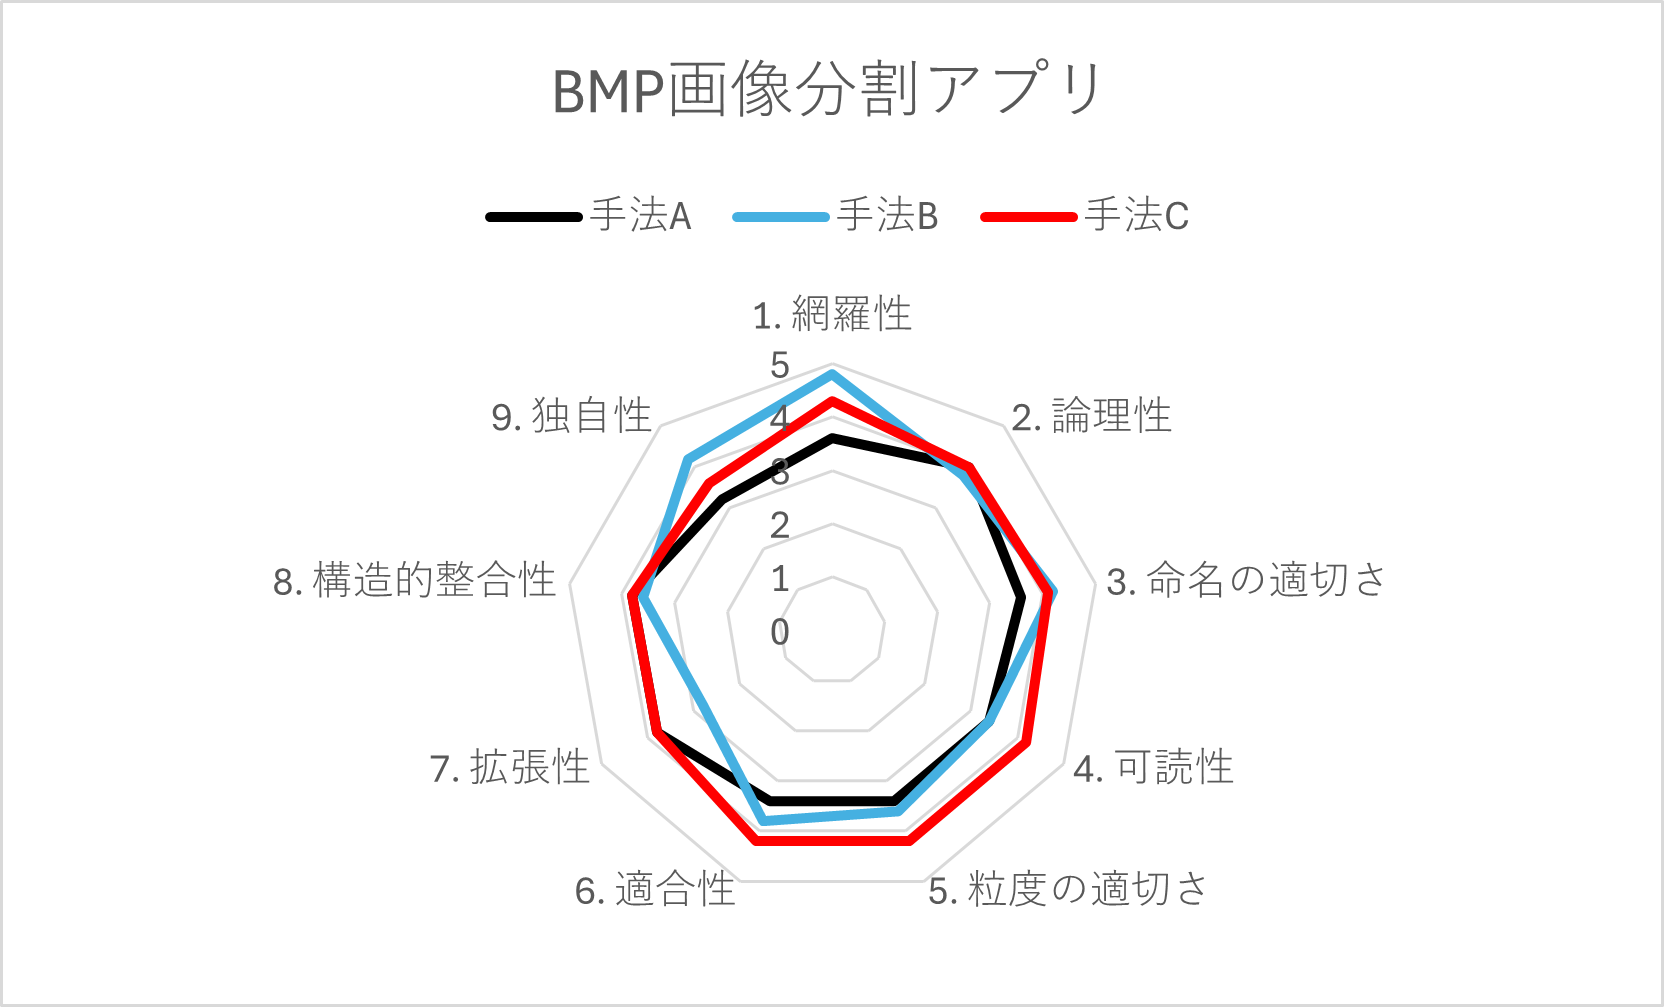
\includegraphics[width=0.8\textwidth]{images/BMPラベル.png}
  \caption{BMP画像分割アプリの評価結果のレーダーチャート}
  \label{fig:bmpchart}
\end{figure}

\begin{figure}[H]
  \centering
  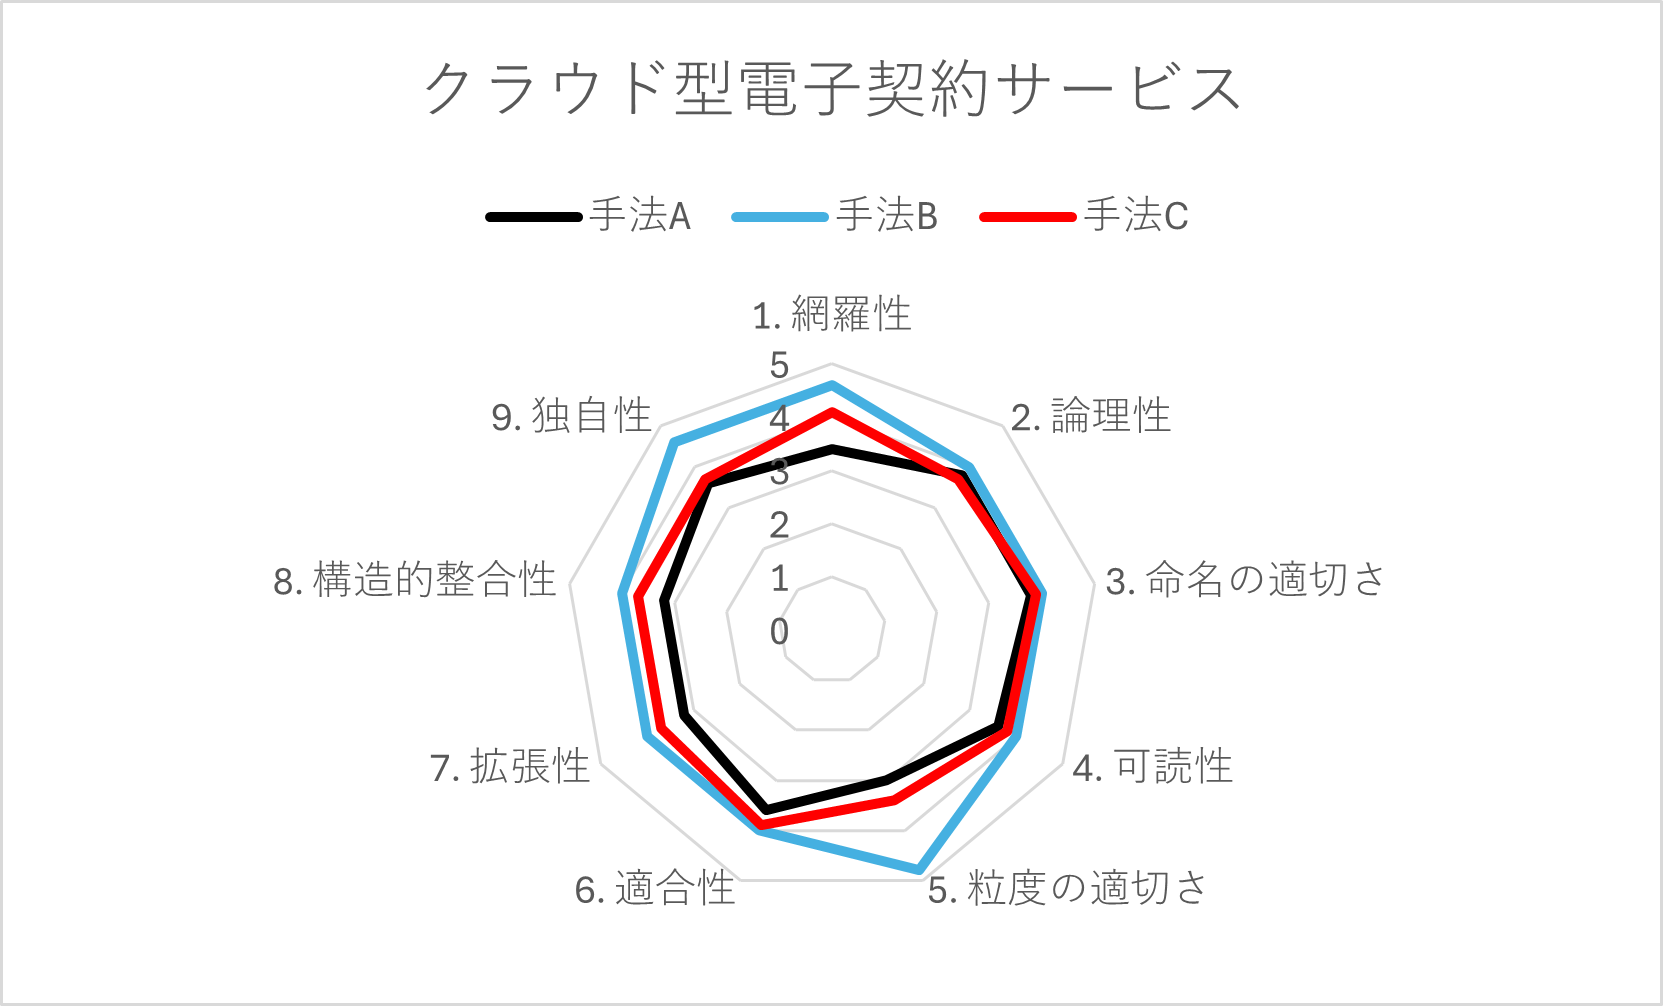
\includegraphics[width=0.8\textwidth]{images/クラウドラベル.png}
  \caption{クラウド型電子契約サービスの評価結果のレーダーチャート}
  \label{fig:cloudchart}
\end{figure}




% \begin{table}[H]
%   \caption{BMP画像分割アプリの評価結果}
%   \label{tb:bmp}
%   \centering
%   \begin{tabular}{|l|c|c|c|c|}
%     \hline
%     \textbf{評価項目} & \textbf{手法A} & \textbf{手法B} & \textbf{被験者Bによる手法C} & \textbf{被験者Dによる手法C} \\
%     \hline\hline
%     1. 網羅性 & 3.6 & 4.8 & 4.4 & 4.2  \\
%     \hline
%     2. 論理性 & 4 & 3.8 & 4.2 & 3.8 \\
%     \hline
%     3. 命名の適切さ & 3.6 & 4.2 & 4.2 & 4  \\
%     \hline
%     4. 可読性 & 3.4 & 3.4 & 4.4 & 4  \\
%     \hline
%     5. 粒度の適切さ & 3.4 & 3.6 & 4.2 & 4.2 \\
%     \hline
%     6. 適合性 & 3.4 & 3.8 & 4.4 & 4 \\
%     \hline
%     7. 拡張性 & 3.8 & 2.8 & 4 & 3.6 \\
%     \hline
%     8. 構造的整合性 & 3.8 & 3.6 & 3 & 4 \\
%     \hline
%     9. 独自性 & 3.2 & 4.2 & 3.6 & 3.6 \\
%     \hline
%   \end{tabular}
% \end{table}

% \begin{table}[H]
%   \caption{クラウド型電子契約サービスの評価結果}
%   \label{tb:cloud}
%   \centering
%   \begin{tabular}{|l|c|c|c|c|}
%     \hline
%     \textbf{評価項目} & \textbf{手法A} & \textbf{手法B} & \textbf{被験者Aによる手法C} & \textbf{被験者Cによる手法C} \\
%     \hline\hline
%     1. 網羅性 & 3.4 & 4.6 & 4 & 4.2  \\
%     \hline
%     2. 論理性 & 3.8 & 4 & 3.6 & 3.8  \\
%     \hline
%     3. 命名の適切さ & 3.8 & 4 & 4 & 3.8  \\
%     \hline
%     4. 可読性 & 3.6 & 4 & 3.8 & 3.8  \\
%     \hline
%     5. 粒度の適切さ & 3 & 4.8 & 2.8 & 4  \\
%     \hline
%     6. 適合性 & 3.6 & 4 & 3.8 & 4  \\
%     \hline
%     7. 拡張性 & 3.2 & 4 & 4 & 3.4 \\
%     \hline
%     8. 構造的整合性 & 3.6 & 4 & 3.8 & 3.6 \\
%     \hline
%     9. 独自性 & 2.8 & 4.6 & 3.8 & 3.6 \\
%     \hline
%   \end{tabular}
% \end{table}















% 本節では、5人の評価者による詳細な評価結果を示す。
% 表\ref{tb:detailed_evaluation_results_A}、表\ref{tb:detailed_evaluation_results_B}、表\ref{tb:detailed_evaluation_results_C}に、各手法で作成された章立てに対する評価者ごとの評価点と、各評価項目の平均値を示す。





% 上記の表より、手法C(提案するプロンプト)がすべての評価項目において最も高い平均スコアを記録していることが分かる。
% 特に「構造的整合性」では全評価者が5点を付けており、提案するプロンプトの有効性が明確に示されている。
% また、評価者間のばらつきも手法Cが最も小さく、安定した品質の章立てが生成されていることが確認できる。

% \section{実験結果}
% 本節では、2つの対象システムについて、各手法で作成した章立ての評価結果を示す。
% システムごとに評価結果の概要を示した後、作成した章立ての詳細と考察を述べる。

% \subsection{BMP画像分割アプリにおける章立ての評価結果}

% \subsubsection{評価結果の概要}
% BMP画像分割アプリについて、手法A(被験者A)、手法B(被験者C)、手法C(被験者BとD)が作成した章立ての評価結果を表\ref{tb:evaluation_result_bmp}に示す。

% \begin{table}[H]
%   \caption{BMP画像分割アプリの評価結果}
%   \label{tb:evaluation_result_bmp}
%   \centering
%   \begin{tabular}{|l|c|c|c|}
%     \hline
%     \textbf{評価項目} & \textbf{手法A} & \textbf{手法B} & \textbf{手法C(平均)} \\
%     \hline\hline
%     1. 網羅性 & 3.5 & 4.0 & \textbf{4.8} \\
%     \hline
%     2. 論理性 & 4.0 & 3.5 & \textbf{4.5} \\
%     \hline
%     3. 命名の適切さ & 3.8 & 3.5 & \textbf{4.2} \\
%     \hline
%     4. 可読性 & 3.2 & 3.8 & \textbf{4.6} \\
%     \hline
%     5. 粒度の適切さ & 3.0 & 2.5 & \textbf{4.0} \\
%     \hline
%     6. 適合性 & 3.5 & 3.5 & \textbf{4.7} \\
%     \hline
%     7. 拡張性 & 3.0 & 3.8 & \textbf{4.3} \\
%     \hline
%     8. 構造的整合性 & 3.8 & 3.2 & \textbf{4.9} \\
%     \hline
%     9. 独自性 & 3.0 & 3.0 & \textbf{4.0} \\
%     \hline
%   \end{tabular}
% \end{table}

% 表\ref{tb:evaluation_result_bmp}より、提案するプロンプトを用いた手法(手法C)がすべての評価項目において最も高いスコアを記録した。
% 特に「網羅性」(4.8)、「可読性」(4.6)、「適合性」(4.7)、「構造的整合性」(4.9)において顕著な高評価を得ており、提案するプロンプトの有効性が確認出来た。
% 手法Aは「論理性」(4.0)において比較的高いスコアを示したが、「粒度の適切さ」(3.0)や「拡張性」(3.0)では低い評価となった。
% 手法Bは全体的に中程度の評価であり、特に「粒度の適切さ」(2.5)と「構造的整合性」(3.2)において改善の余地が見られた。

% \clearpage
% % \begin{minipage}{\textwidth}
% \subsubsection{作成した章立ての詳細}
% 各手法で作成した章立ての詳細を以下に示す。

% \paragraph{手法A(手動作成)による章立て}
% 図\ref{fig:A_chapter_structure_of_bmp_app}に、手法Aで作成した章立てを示す。
% この章立ては、被験者がLLMを使用せず、自身の経験と知識に基づいて作成したものである。



% 全体として9章で構成され、比較的シンプルな構造となっている。
% 「概要」「基本条件」「構成」「機能」「運用」「セキュリティ」「安全設計」「データ仕様」「付帯事項」という基本的な項目は網羅されているが、階層構造が浅く、粒度の適切さに欠ける部分が見られる。
% 特に、第3章「構成」において節番号の付け方に不整合があり(3.1, 3.2ではなく1., 2.となっている)、構造的整合性の評価が低くなった要因と考えられる。
% また、第6章「セキュリティ」と第7章「安全設計」が節レベルの詳細を持たず、拡張性に課題がある。
% % \end{minipage}
% % \clearpage
% \begin{minipage}{\textwidth}
% \paragraph{手法B(自由プロンプト)による章立て}
% 図\ref{fig:B_chapter_structure_of_bmp_app}に、手法Bで作成した章立てを示す。
% この章立ては、被験者がLLMを使用したが、本研究のプロンプトは使用せず、自由な指示で作成したものである。


% \clearpage
% 全体として10章で構成し、手法Aと比較して詳細な階層構造を持つ。
% 「用語・略語定義」や「画像分割処理仕様」など、手法Aにはない独自の章が含んでおり、網羅性が向上している。
% また、各章が適切に節・項に分割されており、可読性が高い。
% しかし、第5章「画像分割処理仕様」が独立した章として存在する一方で、第4章「機能仕様」との関係が不明瞭であり、論理性の評価が低くなった。
% また、粒度の適切さについては、項レベルまで細分化されているものの、内容の粒度が不均一であり、改善の余地がある。

% \clearpage
% \begin{minipage}{\textwidth}
% \paragraph{手法C(提案するプロンプト)による章立て}
% 図\ref{fig:C_chapter_structure_of_bmp_app_1}と図\ref{fig:C_chapter_structure_of_bmp_app_2}に、手法Cを用いて作成した2つの章立てを示す。
% これらは、被験者BとDがそれぞれ本研究のテンプレートプロンプトを用いて作成したものである。




% 両者とも10〜11章で構成され、体系的かつ詳細な階層構造を持つ。
% 共通して「概要」「動作環境・前提条件」「システム全体像/仕様」「画面仕様」「機能仕様」「エラー仕様」「非機能要件」「データ仕様」「運用仕様」「テスト観点」という項目が含まれており、高い網羅性を示している。
% 特に、「ユースケース」「画面仕様」「非機能要件」「テスト観点整理」など、手法AやBにはない項目が含まれており、新人プログラマにとって理解しやすい構成となっている(適合性の高評価)。
% また、章・節・項の階層構造が一貫しており、構造的整合性が非常に高い。
% 2つの章立ての違いとしては、章の順序(「システム全体像」と「動作環境」の順番)や、「ユースケース」の独立性などが挙げられるが、いずれも論理的な構成となっている。

% \clearpage
% \begin{minipage}{\textwidth}
% \subsubsection{考察}
% BMP画像分割アプリの評価結果から、以下の知見が得られた。

% \begin{itemize}
%     \item \textbf{提案するプロンプトの優位性}: 提案するプロンプトを用いた手法(手法C)は、すべての評価項目において最も高いスコアを記録し、特に「網羅性」「適合性」「構造的整合性」において顕著な優位性を示した。これは、テンプレートプロンプトが「ベース章立て」と「出力指示」を明示的に提供することで、体系的かつ一貫性のある章立てを生成できることを示している。
    
%     \item \textbf{手動作成の課題}: 手法Aは、経験に基づいた論理的な構成を示したものの、粒度の適切さや拡張性において課題が見られた。特に、階層構造の不整合(第3章の節番号)は、手動作成における見落としの可能性を示唆している。
    
%     \item \textbf{自由プロンプトの使用の限界}: 手法Bは、手法Aよりも詳細な章立てを生成したが、章の論理的な関係性や粒度の均一性において改善の余地があった。これは、明確な指示がない場合、LLMが生成する章立ての品質にばらつきが生じることを示している。
    
%     \item \textbf{提案するプロンプトの再現性}: 手法Cで作成された2つの章立ては、異なる被験者によって作成されたにもかかわらず、高い類似性と一貫性を示した。これは、テンプレートプロンプトが再現性の高い章立て生成を可能にすることを示している。
% \end{itemize}
% \end{minipage}

% \subsection{クラウド型電子契約サービスにおける章立ての評価結果}

% \subsubsection{評価結果の概要}
% クラウド型電子契約サービスについて、手法A(被験者B)、手法B(被験者D)、手法C(被験者AとC)で作成された章立ての評価結果を表\ref{tb:evaluation_result_cloud}に示す。

% \begin{table}[H]
%   \caption{クラウド型電子契約サービスの評価結果}
%   \label{tb:evaluation_result_cloud}
%   \centering
%   \begin{tabular}{|l|c|c|c|}
%     \hline
%     \textbf{評価項目} & \textbf{手法A} & \textbf{手法B} & \textbf{手法C(提案するプロンプト)} \\
%     \hline\hline
%     1. 網羅性 & 3.5 & 3.5 & \textbf{4.8} \\
%     \hline
%     2. 論理性 & 4.0 & 2.5 & \textbf{4.5} \\
%     \hline
%     3. 命名の適切さ & 3.8 & 3.5 & \textbf{4.2} \\
%     \hline
%     4. 可読性 & 3.2 & 3.2 & \textbf{4.6} \\
%     \hline
%     5. 粒度の適切さ & 3.0 & 2.5 & \textbf{4.0} \\
%     \hline
%     6. 適合性 & 3.5 & 3.0 & \textbf{4.7} \\
%     \hline
%     7. 拡張性 & 3.0 & 3.2 & \textbf{4.3} \\
%     \hline
%     8. 構造的整合性 & 3.8 & 2.8 & \textbf{4.9} \\
%     \hline
%     9. 独自性 & 3.0 & 3.0 & \textbf{4.0} \\
%     \hline 
%   \end{tabular}
% \end{table}

% 表\ref{tb:evaluation_result_cloud}より、BMP画像分割アプリと同様に、提案するプロンプトを用いた手法(手法C)がすべての評価項目において最も高いスコアを記録した。
% 特に「網羅性」(4.8)、「可読性」(4.6)、「適合性」(4.7)、「構造的整合性」(4.9)において顕著な高評価を得ており、システムの複雑さに関わらず提案するプロンプトの有効性が確認された。
% 手法Aは「論理性」(4.0)において比較的高いスコアを示したが、BMP画像分割アプリと同様に「粒度の適切さ」(3.0)や「拡張性」(3.0)では低い評価となった。
% 手法Bは、特に「論理性」(2.5)と「構造的整合性」(2.8)において低い評価を受けており、複雑なシステムにおいて自由プロンプトでの章立て作成の難しさが示された。

% \clearpage
% \subsubsection{作成した章立ての詳細}
% 各手法で作成した章立ての詳細を以下に示す。

% % \begin{minipage}{\textwidth}
% \paragraph{手法A(手動作成)による章立て}
% 図\ref{fig:A_chapter_structure_of_cloud_contract_system}に、手法Aで作成した章立てを示す。


% 全体として9章で構成され、BMP画像分割アプリの手法Aと類似した構造を持つ。
% 「概要」「システム基本条件」「システム構成」「システムの機能」「システムの運用」「セキュリティ」「安全設計」「データ仕様」「付帯事項」という基本的な項目は網羅されているが、クラウドサービス特有の「画面仕様」や「外部インターフェース」などの項目が不足している。
% また、第4章「システムの機能」の項レベル(4.2.1〜4.2.4)において、番号の付け方に不整合があり(スペースがない)、構造的整合性に課題がある。
% 第2章「システム基本条件」の2.6「以降環境」は「移行環境」の誤記と思われ、命名の適切さにも問題が見られる。
% % \end{minipage}

% \clearpage
% \begin{minipage}{\textwidth}
% \paragraph{手法B(自由プロンプト)による章立て}
% 図\ref{fig:B_chapter_structure_of_cloud_contract_system}に、手法Bで作成した章立てを示す。


% \end{minipage}
% \clearpage
% 全体として11章で構成され、非常に詳細な章立てとなっている。
% 「画面仕様」「セキュリティ設計」「安全性・法的要件」「非機能要件」など、クラウド型電子契約サービスに必要な項目が網羅されており、手法Aと比較して高い網羅性を示している。
% 特に、第7章「セキュリティ設計」と第8章「安全性・法的要件」が独立して存在し、電子契約サービスの重要な要素が適切に扱われている。
% しかし、章の配置に論理的な問題が見られる。例えば、第2章「システム基本条件」の2.4「性能・可用性要件」と第10章「非機能要件」の10.1「性能要件」、10.2「可用性要件」が重複しており、情報の整理が不十分である。
% また、第4章「機能仕様」と第5章「画面仕様」の関係が不明瞭であり、論理性の評価が低くなった要因と考えられる。

% \clearpage
% \begin{minipage}{\textwidth}
% \paragraph{手法C(提案するプロンプト)による章立て}
% 図\ref{fig:C_chapter_structure_of_cloud_contract_system_1}と図\ref{fig:C_chapter_structure_of_cloud_contract_system_2}に、手法Cで作成された2つの章立てを示す。


% \end{minipage}


% \clearpage
% \begin{minipage}{\textwidth}
% \end{minipage}

% 両者とも13章で構成され、非常に体系的かつ詳細な階層構造を持つ。
% 共通して「概要」「システム全体像」「動作環境・基本条件」「画面仕様」「機能仕様」「操作フロー」「外部インターフェース/データ仕様」「エラー仕様」「セキュリティ/非機能要件」「運用仕様」「テスト観点」「付録」という項目が含まれており、クラウド型電子契約サービスに必要な要素が網羅されている。
% 特に、「ユースケース」「操作フロー仕様」「外部インターフェース仕様」「テスト観点整理」など、複雑なシステムの理解に必要な項目が適切に配置されており、高い適合性を示している。
% また、章・節・項の階層構造が一貫しており、構造的整合性が非常に高い。
% 2つの章立ての違いとしては、「画面仕様」と「機能仕様」の順序、「セキュリティ仕様」の独立性などが挙げられるが、いずれも論理的な構成となっている。

% \subsubsection{考察}
% クラウド型電子契約サービスの評価結果から、以下の知見が得られた。

% \begin{itemize}
%     \item \textbf{複雑なシステムにおける提案するプロンプトの有効性}: BMP画像分割アプリと同様に、提案するプロンプトを用いた手法(手法C)はすべての評価項目において最も高いスコアを記録した。特に、クラウド型電子契約サービスのような複雑なシステムにおいても、提案するプロンプトが高品質な章立てを生成できることを確認した。
    
%     \item \textbf{システム規模による影響}: クラウド型電子契約サービスは、BMP画像分割アプリと比較してシステム規模が大きく、必要な章立ての項目も多い。手法Bは、BMP画像分割アプリでは比較的良好な評価を得たが、クラウド型電子契約サービスでは論理性と構造的整合性において低い評価を受けた。これは、システムの複雑さが増すほど、明確な指示がない場合のLLMの章立て生成の品質が低下することを示唆している。
    
%     \item \textbf{ドメイン知識の重要性}: 手法Aは、BMP画像分割アプリと同様の構造を採用したが、クラウド型電子契約サービス特有の「画面仕様」や「外部インターフェース」などの項目が不足していた。これは、手動作成においてドメイン知識が重要であることを示している。一方、提案するプロンプトを用いた手法は、テンプレートプロンプトによってドメイン知識を補完し、高品質な章立てを生成できることを確認した。
    
%     \item \textbf{提案するプロンプトの柔軟性}: 手法Cを用いて作成した2つの章立ては、章の順序や項目の配置に若干の違いがあるものの、いずれも高い評価を得た。これは、テンプレートプロンプトが一定の柔軟性を持ちながらも、品質を保証できることを示している。
% \end{itemize}

% \subsection{実験結果の分析}

% \subsubsection{全体的な傾向}
% 2つのシステムにおける評価結果を総合的に比較した結果を、表\ref{tb:evaluation_result_summary}に示す。

% \begin{table}[H]
%   \caption{全体の評価結果の平均}
%   \label{tb:evaluation_result_summary}
%   \centering
%   \begin{tabular}{|l|c|c|c|}
%     \hline
%     \textbf{評価項目} & \textbf{手法A} & \textbf{手法B} & \textbf{手法C} \\
%     \hline\hline
%     1. 網羅性 & 3.5 & 3.8 & \textbf{4.8} \\
%     \hline
%     2. 論理性 & 4.0 & 3.0 & \textbf{4.5} \\
%     \hline
%     3. 命名の適切さ & 3.8 & 3.5 & \textbf{4.2} \\
%     \hline
%     4. 可読性 & 3.2 & 3.5 & \textbf{4.6} \\
%     \hline
%     5. 粒度の適切さ & 3.0 & 2.5 & \textbf{4.0} \\
%     \hline
%     6. 適合性 & 3.5 & 3.2 & \textbf{4.7} \\
%     \hline
%     7. 拡張性 & 3.0 & 3.5 & \textbf{4.3} \\
%     \hline
%     8. 構造的整合性 & 3.8 & 3.0 & \textbf{4.9} \\
%     \hline
%   \end{tabular}
% \end{table}

% 図\ref{fig:result_chart}に、各手法の評価結果をレーダーチャートで比較したものを示す。

% \begin{figure}[H]
%   \centering
%   % TODO: ここにExcel等で作成したレーダーチャートの画像を差し替える (images/result_chart.pdf)
%   \includegraphics[width=0.8\linewidth]{images/syokuji_computer.png} % 仮の画像
%   \caption{実験結果の比較(レーダーチャート)}
%   \label{fig:result_chart}
% \end{figure}

% \subsubsection{提案するプロンプトの有効性}
% 実験の結果、提案するプロンプトを用いた手法(手法C)は、すべての評価項目において手法Aおよび手法Bを上回るスコアを記録した。
% 特に「網羅性」(4.8)、「可読性」(4.6)、「適合性」(4.7)、「構造的整合性」(4.9)において顕著な高さを示しており、これはプロンプトで与えた「ベース章立て」と「出力指示」の有効性を示唆している。

% 提案するプロンプトの優位性は、以下の要因によるものと考えられる：

% \begin{enumerate}
%     \item \textbf{体系的な構造}: テンプレートプロンプトが提供する「ベース章立て」により、システム仕様書に必要な項目が網羅的に含まれる。
    
%     \item \textbf{一貫性の確保}: 「出力指示」により、章・節・項の階層構造が一貫して適用され、構造的整合性が高まる。
    
%     \item \textbf{ドメイン知識の補完}: テンプレートプロンプトが、システム仕様書作成に必要なドメイン知識を提供し、経験の浅い被験者でも高品質な章立てを作成できる。
    
%     \item \textbf{再現性の高さ}: 異なる被験者が同じテンプレートプロンプトを使用することで、類似した高品質な章立てが生成出来る。
% \end{enumerate}

% \subsubsection{手法間の比較}
% 手法A(手動作成)は、「論理性」において比較的高いスコアを示したが、「粒度の適切さ」や「拡張性」では低い評価となった。
% これは、経験に基づいた論理的な構成は可能であるものの、詳細な階層構造の設計や将来の拡張を考慮した設計には課題があることを示している。

% 手法B(自由プロンプト)は、全体的に中程度の評価であり、特に「粒度の適切さ」と「構造的整合性」において改善の余地が見られた。
% また、システムの複雑さが増すほど、論理性の評価が低下する傾向が見られた。
% これは、明確な指示がない場合、LLMが生成する章立ての品質にばらつきが生じることを示している。



% 考察
\chapter{考察}\label{cha:Discussion}

本章では、第5章で得られた評価結果に基づき、提案プロンプトの有用性と特性について考察する。
具体的には、手法A(手動作成)および手法B(自由プロンプト)との比較を通じて、手法C(提案プロンプト)が章立ての品質に与える影響を分析する。
また、プロンプトの構成要素が果たした役割や、対象システムの複雑さが生成結果に与える影響についても議論する。
さらに、関連研究についても述べる。

\section{関連研究}

本節では、本研究と関連する研究について述べる。

Zhu氏らは、LLMを活用して、要求定義書や要件定義書、会議の議事録といった自然言語で書かれたドキュメントから、ソフトウェア要求仕様書(本研究でのシステム仕様書に相当)を自動生成するエージェントであるREQINONEを開発した\cite{reference}。
REQINONEは、入力となるドキュメントから情報を要約、抽出、整形して、あらかじめ用意された章立てテンプレートの、どの章、節に整形した情報を配置するかを決めることで、ソフトウェア要求仕様書の自動生成を実現している。
したがって、このエージェント内では、章立ての自動生成は行われていない。
つまり、テンプレートとなる章立てを人間が事前に用意する必要がある。

一方、本研究で提案するプロンプトは、章立てそのものを自動生成することを目的としている。
% REQINONEが用意された章立てテンプレートに詳細な文書から情報を要約、抽出し、適切な章、節に配置するのに対し、
% 本研究では、システム名と短文のシステム概要のみを入力として、
% 対象システムに適した章立てを生成する。
% これにより、開発の初期段階において、詳細な要求定義書や要件定義書、会議の議事録が存在しない状況でも、
% システム仕様書の骨格となる章立てを作成できる点が本研究の特長である。

% また、REQINONEは膨大な入力文書を必要とするため、情報が十分に揃った状況での利用を想定している。
% 一方、本研究のプロンプトは最小限の情報で章立てを生成できるため、
% プロジェクトの初期段階から活用でき、REQINONEとは補完的な関係にあると言える。
したがって、REQINONEと本研究で提案するプロンプトは、補完的な関係にあると言える。

% 上前氏らは、LLMを用いてマニュアルの目次(章立て)を自動生成のための情報分類と順序付けの手法を提案している。
% 上前氏らの手法では、目次作成のプロセスをページ分類選択と順序付けの2段階に分け、目次の生成を行っている。
% 入力には、ページと呼ばれるマニュアルの目次に掲載されるページ集合を入力としている。
% 上前氏らの研究におけるページとは、タイトルと本文の組み合わせである。

\section{章立ての評価者による評価結果に対する分析}

% \addtocontents{toc}{\protect\setcounter{tocdepth}{1}}
\subsection{手法A(手動作成)と手法C(提案プロンプト)で作成した章立ての評価結果の分析}
% \addtocontents{toc}{\protect\setcounter{tocdepth}{2}}

実験結果より、手法C(提案プロンプト)は、手法A(手動作成)と比較して、多くの評価項目で高い点数を獲得した(表\ref{tb:bmp}、表\ref{tb:cloud}参照)。
特に「網羅性」「可読性」「独自性」の項目において、優位性がある。

BMP画像分割アプリの結果(表\ref{tb:bmp})において、手法C(提案プロンプト)は評価項目のすべてにおいて、手法A(手動作成)を上回った。特に、手法A(手動作成)の網羅性が3.6点であったのに対し、手法C(提案プロンプト)は4.3点と高い評価を得た。
これは、システム開発の経験が浅い作成者は、「用語定義」や「テスト観点」といった項目を漏らしてしまう傾向があり、被験者Aの結果もこれを裏付けている。
実際に、評価者からは手法A(手動作成)に対し「書くべきことが書けていない」や「シンプル」といった、内容の不足や具体性の欠如を指摘するコメントがあった。
一方、提案プロンプトを用いることで、ベース章立てテンプレートと役割付与により、抜け漏れが少ない章立てを生成したと考える。
実際に手法C(提案プロンプト)に対しては、「一番整理されている」「構成が分かりやすくていい」といった、論理的で整理された構造を高く評価するコメントがあった。

クラウド型電子契約サービスの結果(表\ref{tb:cloud})においては、論理性以外のすべての評価項目で手法A(手動作成)を上回った。特に「独自性」において手法C(提案プロンプト)(3.7点)は手法A(手動作成)(2.8点)を大きく上回った。
手動作成では、対象とするシステムに対する知識が不足している場合(例えばクラウドサービスのセキュリティ要件や電子署名の法的要件など)、システム固有の詳細な項目を書き出すことが困難である。
一方、提案プロンプトを用いることで、LLMが持つ広範な知識を活用し、作成者の知識の不足を補完することで、独自性の高い章立てが可能となったと考察する。

クラウド型電子契約サービスにおいても、手法A(手動作成)に対し評価者から「粒度が荒すぎる上に項目として不足箇所が多い」「章立てが荒く、記載が不足している」というコメントがあったのに対し、手法C(提案プロンプト)は「必要なことが書かれている」「拡張しやすそう」という評価を得ており、提案プロンプトが網羅性と将来の拡張性の両立に寄与していることを示した。
これは、提案プロンプトのベース章立てテンプレートと出力指示により、章、節、項の階層構造が明確になり、読みやすく整理された構成を出力した結果であると考察する。
実際に「可読性」に関しても、手法C(提案プロンプト)はBMP画像分割アプリの章立てで4.2点、クラウド型電子契約サービスの章立てで3.8点と、手法A(手動作成)(BMP: 3.4点、クラウド: 3.6点)を上回っている。

% 以上のことから、提案プロンプトは、特に仕様書作成の経験が浅い作成者にとって、手動作成よりも高品質でバランスの取れた章立てを作成するための強力な支援ツールとなると言える。

\subsection{手法B(自由プロンプト)と手法C(提案プロンプト)で作成した章立ての評価結果の分析}
手法B(自由プロンプト)と、手法C(提案プロンプト)の比較からは、提案プロンプトの「安定性」と「品質の均一化」の効果が確認できた。

BMP画像分割アプリにおいて、手法B(自由プロンプト)(被験者C)は網羅性で4.8点という非常に高い点数を記録したが、拡張性は2.8点であった。
また、手法B(自由プロンプト)には複数の評価者から「冗長」というコメントがあった。
これは、「網羅性」や「独自性」が高い一方で、実務上の使い勝手や情報の整理状況において課題があることを示している。
一方で、手法C(提案プロンプト)は網羅性4.3点、拡張性3.8点と、両項目で高い評価を得ており、評価者からは、「一番バランスが良い」「一番拡張性は高く使い勝手は一番よさそう」という評価を得ている。
これは、自由プロンプト特有の「過剰な生成」による拡張性の低下を、提案プロンプトの制約(テンプレートやシステム仕様書の定義)が適切に抑制し、品質の安定化に寄与した結果であると言える。

クラウド型電子契約サービスにおいて、手法B(自由プロンプト)(被験者D)は粒度の適切さで4.8点、独自性で4.6点と極めて高い評価を得た。
これは、被験者Dが少ない制約で自由度を与えたことで、LLMがその能力を最大限に発揮し、クラウドサービス特有の要件を網羅した詳細な仕様書を作成できた例である。
% これに対し、手法C(提案プロンプト)は粒度の適切さ3.4点、独自性3.7点と、手法B(自由プロンプト)には及ばない項目もあった。
% しかし、手法B(自由プロンプト)の論理性や構造的整合性が3点台後半から4.0点と評価者によってばらつきが見られたのに対し、手法C(提案プロンプト)は概ね安定した評価を得ている。

また、手法B(自由プロンプト)において、BMP画像分割アプリの合計点数は34.2点、クラウド型電子契約サービスの合計点数は38.0点であり、その差は3.8点であった。
一方で、手法C(提案プロンプト)の合計点数はそれぞれ36.2点、33.9点であり、その差は2.3点であった。
これは、手法B(自由プロンプト)は対象とするシステムに応じて、品質のばらつきが大きく、手法C(提案プロンプト)は品質のばらつきが少ないことを示している。


\section{IEEE830に基づく章立ての評価とその分析}

表\ref{tb:ieeee}は、IEEE830がシステム仕様書の章立てに含むことを推奨する項目(図\ref{fig:ieee830}参照)と評価実験で作成した章立て(\ref{sec:evaluation_results}節を参照)を比較し、各章立てがIEEE830がシステム仕様書の章立てに含むことを推奨する項目をどれだけ満たしているかを示した表である。
この表から、BMP画像分割アプリを対象として手法Aで作成した章立て(図\ref{fig:A_chapter_structure_of_bmp_app}参照)は、IEEE830がシステム仕様書の章立てに含むことを推奨する項目を36項目中11項目(30.6\%)満たしていることが分かる。
また、BMP画像分割アプリを対象として手法Bで作成した章立て(図\ref{fig:B_chapter_structure_of_bmp_app}参照)は、36項目中13項目(36.1\%)満たしていることが分かる。
また、BMP画像分割アプリを対象として被験者Bが手法Cで作成した章立て(図\ref{fig:C_chapter_structure_of_bmp_app_1})は、36項目中16項目(44.4\%)満たしていることが分かる。
また、BMP画像分割アプリを対象として被験者Dが手法Cで作成した章立て(図\ref{fig:C_chapter_structure_of_bmp_app_2})は、36項目中16項目(44.4\%)満たしていることが分かる。
また、クラウド型電子契約サービスを対象として手法Aで作成した章立て(図\ref{fig:A_chapter_structure_of_cloud_contract_system}参照)は、IEEE830がシステム仕様書の章立てに含むことを推奨する項目を36項目中14項目(38.9\%)満たしていることが分かる。
また、クラウド型電子契約サービスを対象として手法Bで作成した章立て(図\ref{fig:B_chapter_structure_of_cloud_contract_system}参照)は、36項目中26項目(72.2\%)満たしていることが分かる。
また、クラウド型電子契約サービスを対象として被験者Aが手法Cで作成した章立て(図\ref{fig:C_chapter_structure_of_cloud_contract_system_1})は、36項目中24項目(66.7\%)満たしていることが分かる。
また、クラウド型電子契約サービスを対象として被験者Cが手法Cで作成した章立て(図\ref{fig:C_chapter_structure_of_cloud_contract_system_2})は、36項目中22項目(61.1\%)満たしていることが分かる。

この結果から、手法C(提案プロンプト)は、手法A(手動作成)と比較して、IEEE830がシステム仕様書の章立てに含むことを推奨する項目を多く満たしていることが分かる。
また、手法C(提案プロンプト)のBMP画像分割アプリとクラウド型電子契約サービスの差は、8項目であるのに対し、手法B(自由プロンプト)の差は13項目である。
したがって、手法C(提案プロンプト)は、手法B(自由プロンプト)と比較して、対象システムの違いによる章立ての品質のばらつきが少ないことが分かる。

また、手法C(提案プロンプト)は、BMP画像分割アプリにおいて、平均の網羅率が44.4\%であり、クラウド型電子契約サービスにおいては、平均の網羅率が63.9\%である。
今回の提案プロンプトの「システム仕様書の定義」の中に目的として、「システムテスト担当者がテスト項目を作るために参照する文書」という項目を入れたが、これらの網羅率の数値は、テスト設計の網羅性という観点において、不十分な数値だと考える。
したがって、テスト設計の網羅性を向上させるために、「システム仕様書の定義」の記述を改善する必要があると考察する。

\begin{table}[tp]
  \centering
  \caption{IEEE830の章立てに含むことが推奨される項目と評価実験で作成した章立ての比較}
  \label{tb:ieeee}
%   \footnotesize
%   \renewcommand{\arraystretch}{1.2}
  \scriptsize
  \renewcommand{\arraystretch}{0.7}
  \setlength{\tabcolsep}{2pt}
  \begin{tabular}{|l|c|c|c|c|c|c|c|c|c|}
    \hline
    \textbf{仕様書の章立て項目} &\begin{tabular}{c} \textbf{手法A}\\\textbf{(BMP)} \\ \end{tabular}& \begin{tabular}{c} \textbf{手法B}\\\textbf{(BMP)} \\ \end{tabular}& \begin{tabular}{c} \textbf{手法C}\\\textbf{(BMP,}\\\textbf{被験者B)} \\ \end{tabular}& \begin{tabular}{c} \textbf{手法C}\\\textbf{(BMP,}\\\textbf{被験者D)} \\ \end{tabular}& \begin{tabular}{c} \textbf{手法A}\\\textbf{(電子契約)} \\ \end{tabular}& \begin{tabular}{c} \textbf{手法B}\\\textbf{(電子契約)} \\ \end{tabular}& \begin{tabular}{c} \textbf{手法C}\\\textbf{(電子契約,}\\\textbf{被験者A)} \\ \end{tabular}& \begin{tabular}{c} \textbf{手法C}\\\textbf{(電子契約,}\\\textbf{被験者C)} \\ \end{tabular}\\ \hline
    1. はじめに & 〇& 〇& 〇& 〇& 〇& 〇& 〇& 〇 \\ \hline
    \forceindent1.1 本書の目的 & 〇& 〇& 〇& 〇& 〇& 〇& 〇& 〇 \\ \hline
    \forceindent1.2 対象範囲 & & & 〇& 〇& 〇& 〇& 〇& 〇 \\ \hline
    \forceindent1.3 用語定義・略語 &〇 & 〇& 〇& 〇&〇 & & & \\ \hline
    \forceindent1.4 本書の構成 & &〇 &〇 &〇 & &〇 & 〇&〇 \\ \hline
    2. システム概要 &〇 & 〇& 〇& 〇&〇 & 〇& 〇& 〇\\ \hline
    \forceindent2.1 システムの全体像 & & 〇& 〇& 〇& &〇 &〇 & 〇\\ \hline
    \forceindent\forceindent2.1.1 システム間インターフェース & & & & & & & & \\ \hline
    \forceindent\forceindent2.1.2 画面インターフェース & & & & & & & & \\ \hline
    \forceindent\forceindent2.1.3 ハードウェア構成 & & & & & 〇& &〇 & \\ \hline
    \forceindent\forceindent2.1.4 ソフトウェア構成 &〇 & & & & 〇& 〇& 〇&〇 \\ \hline
    \forceindent\forceindent2.1.5 ネットワーク構成 &〇 & & & & 〇& 〇& 〇&〇 \\ \hline
    \forceindent\forceindent2.1.6 リソース制約 & & & & & & & & \\ \hline
    \forceindent\forceindent2.1.7 運用環境 &〇 & 〇&〇 &〇 & & 〇& 〇&〇 \\ \hline
    \forceindent\forceindent2.1.8 設置条件 & & & & & & & & \\ \hline
    \forceindent2.2 システムの主な機能 &〇 &〇 &〇 &〇 &〇 & 〇& 〇& 〇\\ \hline
    \forceindent2.3 想定利用者 & & & 〇& 〇& & 〇& 〇&〇 \\ \hline
    \forceindent2.4 制約事項 & &〇 &〇 &〇 & &〇 & 〇& 〇\\ \hline
    \forceindent2.5 前提条件および依存関係 & & &〇 & 〇& & 〇& 〇& 〇\\ \hline
    \forceindent2.6 将来対応事項 & & 〇& & & & & 〇& \\ \hline
    3. 詳細要件 & & &〇 & 〇&〇 & & 〇& 〇\\ \hline
    \forceindent3.1 外部インターフェース仕様 & & & & & &〇 &〇 & \\ \hline
    \forceindent3.2 機能要件 &〇 &〇 &〇 &〇 &〇 &〇 &〇 &〇 \\ \hline
    \forceindent3.3 性能要件 & &〇 &〇 &〇 & &〇 &〇 &〇 \\ \hline
    \forceindent3.4 データベース要件 &〇 & & & & &〇 &〇 & 〇\\ \hline
    \forceindent3.5 設計上の制約事項 & & & & &〇 & & & \\ \hline
    \forceindent3.6 システム品質特性 & & & & & &〇 & & \\ \hline
    \forceindent\forceindent3.6.1 信頼性 & & & & & & 〇& & \\ \hline
    \forceindent\forceindent3.6.2 可用性 & &  & & & & 〇& 〇&〇 \\ \hline
    \forceindent\forceindent3.6.3 セキュリティ &〇 &〇 &〇 &〇 &〇 &〇 & 〇& 〇\\ \hline
    \forceindent\forceindent3.6.4 保守性 & & & & & & 〇&〇 & \\ \hline
    \forceindent\forceindent3.6.5 移植性 & & & & &〇 &〇 & & \\ \hline
    \forceindent3.7 その他の要件 & & &〇 & 〇&〇 &〇 & 〇& 〇\\ \hline
    4. 参考資料 & & & & & &〇 & &〇 \\ \hline
    \forceindent4.1 索引 & & & & & & & & \\ \hline
    \forceindent4.2 付録 &〇 &〇 & & &〇 & &〇 & 〇\\ \hline
    \textbf{合計} & \textbf{11}& \textbf{13}& \textbf{16}& \textbf{16}& \textbf{14}& \textbf{26}& \textbf{24}& \textbf{22}\\ \hline
  \end{tabular}
\end{table}

\section{プロンプトに対する分析}
\subsection{提案プロンプトの構成要素の寄与}

% 提案するプロンプトの構成要素が生成結果に与える影響を確認するため、図\ref{fig:base_prompt}をベースプロンプトとして、図\ref{fig:prompt_structure}に示した各構成要素のみを追加したプロンプト5つを作成し、それぞれを用いて章立てを生成した。
提案プロンプトの構成要素が生成結果に与える影響を確認するため、「開発するシステム情報」と「出力指示」からなるプロンプトをベースプロンプトとして作成する。
そして、ベースプロンプトに図\ref{fig:prompt_structure}に示したそれぞれの構成要素のみを追加したプロンプトを5つ作成し、それぞれを用いて章立てを生成する。

図\ref{fig:base_prompt}に、クラウド型電子契約サービスを対象としたベースプロンプトを示す。
なお、ベースプロンプトに「開発するシステム情報」を含む理由は、章立ての生成に最低限必要な情報であるためであり、出力指示を含む理由は、章立ての生成に最低限必要な指示と生成結果に章立て以外のものを含まないようにするためである。

\begin{figure}[tp]
\begin{tcolorbox}[
  colback=white,
  colframe=blue,
  fonttitle=\bfseries
]
\footnotesize
\ttfamily
\fontsize{8}{9}\selectfont
\begin{verbatim}
【開発するシステム情報】
- システム名：クラウド型電子契約サービス
- 概要：PDF技術を活かした電子契約／ワークフロー、それらに付随する文書管理、及びユーザー管理機能を持つクラウドサービス

【出力指示】
・上記情報に基づき、開発するシステムのシステム仕様書に必要な章立てを出力してください。
・ここでいう章立ては、以下の内容を含みます。
　・章と節、章タイトル、節タイトル、項、項タイトル 
・出力形式は**マークダウンの番号付きリスト**としてください。 
・章名以外(目的・記述のポイントなど)は一切書かないでください。
\end{verbatim}
\end{tcolorbox}
\caption{ベースプロンプト}
\label{fig:base_prompt}
\end{figure}

図\ref{fig:base_prompt_outline}に、ベースプロンプトを用いて生成した章立てを示す。

\begin{figure}[tp]
\begin{tcolorbox}[
  colback=white,
  colframe=orange,
  fonttitle=\bfseries
]
\begin{multicols}{2}
\footnotesize
\ttfamily
\fontsize{7}{8}\selectfont
\begin{verbatim}
1. システム概要
   1.1 システム目的
   1.2 システム範囲
   1.3 用語定義
   1.4 前提条件・制約事項

2. 全体構成
   2.1 システムアーキテクチャ
   2.2 構成要素一覧
   2.3 外部システム連携概要
   2.4 ネットワーク構成

3. 機能要件
   3.1 電子契約機能
   3.2 ワークフロー機能
   3.3 文書管理機能
   3.4 ユーザー管理機能
   3.5 管理者機能

4. 画面仕様
   4.1 画面一覧
   4.2 画面遷移図
   4.3 各画面仕様

5. データ仕様
   5.1 データモデル
   5.2 エンティティ定義
   5.3 データ項目定義
   5.4 データ保持方針

6. インターフェース仕様
   6.1 外部連携インターフェース
   6.2 API仕様
   6.3 ファイル入出力仕様

7. セキュリティ仕様
   7.1 認証・認可
   7.2 アクセス制御
   7.3 ログ管理
   7.4 データ暗号化

8. 非機能要件
   8.1 性能要件
   8.2 可用性要件
   8.3 拡張性要件
   8.4 運用性要件

9. 運用・保守仕様
   9.1 運用フロー
   9.2 バックアップ・リストア
   9.3 障害対応
   9.4 監視仕様

10. テスト仕様
    10.1 テスト方針
    10.2 テスト項目一覧
    10.3 受入テスト基準

11. 付録
    11.1 用語集
    11.2 参考資料
    11.3 改訂履歴

\end{verbatim}
\end{multicols}
\end{tcolorbox}
\caption{ベースプロンプトによる章立て}
\label{fig:base_prompt_outline}
\end{figure}

図\ref{fig:only_role}に、ベースプロンプトに役割付与のみを加えたプロンプトを示す。
また、図\ref{fig:only_role_outline}に、図\ref{fig:only_role}に示したプロンプトを用いて生成した章立てを示す。

図\ref{fig:base_prompt_outline}と図\ref{fig:only_role_outline}を比較すると、役割付与の追加により、節の項目が増加し、より網羅的な章立てになっていることが分かる。
具体的には、ベースプロンプトでは節が41個であったのに対し、役割付与を追加すると節が50個になっている。
これは、役割付与が章立ての網羅性の向上に寄与していることを示している。

\begin{figure}[tp]
\begin{tcolorbox}[
  colback=white,
  colframe=blue,
  fonttitle=\bfseries
]
\footnotesize
\ttfamily
\fontsize{8}{9}\selectfont
\begin{verbatim}
あなたはシステム仕様書作成の専門アシスタントです。


【開発するシステム情報】
- システム名：クラウド型電子契約サービス
- 概要：PDF技術を活かした電子契約／ワークフロー、それらに付随する文書管理、及びユーザー管理機能を持つクラウドサービス

【出力指示】
・上記情報に基づき、開発するシステムのシステム仕様書に必要な章立てを出力してください。
・ここでいう章立ては、以下の内容を含みます。
　・章と節、章タイトル、節タイトル、項、項タイトル 
・出力形式は**マークダウンの番号付きリスト**としてください。 
・章名以外(目的・記述のポイントなど)は一切書かないでください。
\end{verbatim}
\end{tcolorbox}
\caption{ベースプロンプトに役割付与のみを加えたプロンプト}
\label{fig:only_role}
\end{figure}



\begin{figure}[tp]
\begin{tcolorbox}[
  colback=white,
  colframe=orange,
  fonttitle=\bfseries
]
\begin{multicols}{2}
\footnotesize
\ttfamily
\fontsize{7}{8}\selectfont
\begin{verbatim}
1. システム概要
   1.1 目的
   1.2 適用範囲
   1.3 用語定義
   1.4 参照資料
   1.5 前提条件
   1.6 制約事項

2. 全体構成
   2.1 システム全体像
   2.2 システム構成図
   2.3 ネットワーク構成
   2.4 ソフトウェア構成
   2.5 ハードウェア構成

3. 機能仕様
   3.1 ユーザー管理機能
   3.2 文書管理機能
   3.3 電子契約機能
   3.4 ワークフロー機能
   3.5 通知機能
   3.6 検索・参照機能
   3.7 ログ管理機能
   3.8 権限管理機能

4. 画面仕様
   4.1 画面一覧
   4.2 画面遷移図
   4.3 画面レイアウト

5. データ仕様
   5.1 データモデル
   5.2 ER図
   5.3 テーブル定義
   5.4 インデックス定義
   5.5 データ保持ポリシー

6. 外部インターフェース仕様
   6.1 外部システム連携
   6.2 API仕様
   6.3 ファイル連携仕様

7. 非機能要件
   7.1 性能要件
   7.2 可用性要件
   7.3 拡張性要件
   7.4 セキュリティ要件
   7.5 バックアップ・リカバリ要件

8. 運用・保守仕様
   8.1 運用体制
   8.2 監視仕様
   8.3 障害対応
   8.4 バージョン管理
   8.5 保守対応

9. テスト仕様
   9.1 テスト方針
   9.2 テスト項目
   9.3 テスト環境
   9.4 受入テスト基準

10. セキュリティ仕様
    10.1 認証方式
    10.2 認可方式
    10.3 通信暗号化
    10.4 ログ監査

11. 制限事項
    11.1 システム制限
    11.2 運用上の制限

\end{verbatim}
\end{multicols}
\end{tcolorbox}
\caption{役割付与のみを加えたプロンプトによる章立て}
\label{fig:only_role_outline}
\end{figure}

図\ref{fig:only_outline}に、図\ref{fig:base_prompt}のベースプロンプトにベースの章立てのみを加えたプロンプトを示す。
また、図\ref{fig:only_outline_outline}に、図\ref{fig:only_outline}に示したプロンプトを用いて生成した章立てを示す。

図\ref{fig:base_prompt_outline}と図\ref{fig:only_outline_outline}を比較すると、ベースの章立てを追加したことにより、「1.概要」、「4.システム基本条件」のように、章タイトルがテンプレートに沿った命名になっていることが分かる。
これは、評価項目の命名の適切さにおいて、BMP画像分割アプリで4.1点(表\ref{tb:bmp})、電子契約サービスで3.9点(表\ref{tb:cloud})という高い評価を得た要因になっていると考える。
一方で、図\ref{fig:only_role_outline}に示した役割付与のみを行った場合と図\ref{fig:only_outline_outline}を比較すると、役割付与のみを追加した場合の章立てには、9章に「テスト仕様」があるが、ベースの章立てを追加した場合の章立てには、「テスト仕様」は存在しない。
これは、ベースの章立てを与えることにより、テンプレートに含まれていない項目がLLMによって生成されにくくなる可能性があることを示唆している。

\begin{figure}[tp]
\begin{tcolorbox}[
  colback=white,
  colframe=blue,
  fonttitle=\bfseries
]
\footnotesize
\ttfamily
\fontsize{8}{9}\selectfont
\begin{verbatim}
【ベース章立てテンプレート(参考)】
1. 概要
 1.1.目的
 1.2.システム概要
 1.3.適用範囲
2. システム基本条件
 2.1.稼働条件
 2.2.他システムインターフェース
 2.3.性能条件
 2.4.拡張条件
 2.5.継承条件
 2.6.以降環境
3. システム構成
 3.1.ハードウェア構成及びネットワーク構成
 3.2.ソフトウェア構成
4. システムの機能
 4.1.機能構成
 4.2.個別機能概要
5. システムの運用
 5.1.運用方法
 5.2.各業務(機能)の運用
 5.3.障害時の運用
6.セキュリティ
7.安全設計
8.データ仕様
 8.1.コード体系
 8.2.データベース
 8.3.ファイル
 8.4.入出力データ
 8.5.メッセージ
9.付帯事項

※ベース章立てはあくまで参考です。必要に応じて章の追加・削除・順序変更を行って、漏れなく体系的な章立てを作成してください。

【開発するシステム情報】
- システム名：クラウド型電子契約サービス
- 概要：PDF技術を活かした電子契約／ワークフロー、それらに付随する文書管理、及びユーザー管理機能を持つクラウドサービス

【出力指示】
・上記情報に基づき、開発するシステムのシステム仕様書に必要な章立てを出力してください。
・ここでいう章立ては、以下の内容を含みます。
　・章と節、章タイトル、節タイトル、項、項タイトル 
・出力形式は**マークダウンの番号付きリスト**としてください。 
・章名以外(目的・記述のポイントなど)は一切書かないでください。

\end{verbatim}
\end{tcolorbox}
\caption{ベースプロンプトにベースの章立てのみを加えたプロンプト}
\label{fig:only_outline}
\end{figure}

\begin{figure}[tp]
\begin{tcolorbox}[
  colback=white,
  colframe=orange,
  fonttitle=\bfseries
]
\begin{multicols}{2}
\footnotesize
\ttfamily
\fontsize{7}{8}\selectfont
\begin{verbatim}
1. 概要
   1.1. 目的
   1.2. システム概要
   1.3. 用語定義
   1.4. 適用範囲

2. 関連資料・前提条件
   2.1. 関連法規・ガイドライン
   2.2. 前提条件
   2.3. 制約条件

3. システム全体構成
   3.1. サービス全体構成
   3.2. ハードウェア構成及びネットワーク構成
   3.3. ソフトウェア構成
   3.4. 外部サービス構成

4. システム基本条件
   4.1. 稼働条件
   4.2. 性能条件
   4.3. 可用性条件
   4.4. 拡張条件
   4.5. 移行条件

5. システム機能要件
   5.1. 機能構成
   5.2. ユーザー管理機能
     5.2.1. ユーザー登録・変更・削除
     5.2.2. ロール・権限管理
     5.2.3. 認証・認可
   5.3. 電子契約機能
     5.3.1. 契約書作成・アップロード
     5.3.2. 署名依頼ワークフロー
     5.3.3. 電子署名・タイムスタンプ付与
     5.3.4. 署名進捗管理
   5.4. ワークフロー機能
     5.4.1. 承認経路設定
     5.4.2. 承認・差戻し・却下
   5.5. 文書管理機能
     5.5.1. 文書保管
     5.5.2. 検索・閲覧
     5.5.3. バージョン管理
   5.6. 通知機能
     5.6.1. メール通知
     5.6.2. 画面通知
   5.7. ログ管理機能
     5.7.1. 操作ログ
     5.7.2. 監査ログ

6. 外部システムインターフェース
   6.1. 外部認証基盤連携
   6.2. 外部署名サービス連携
   6.3. 外部ストレージ連携
   6.4. API連携

7. 非機能要件
   7.1. 性能要件
   7.2. 可用性要件
   7.3. 信頼性要件
   7.4. 拡張性要件
   7.5. 運用保守性要件

8. セキュリティ要件
   8.1. 認証方式
   8.2. アクセス制御
   8.3. データ暗号化
   8.4. 通信暗号化
   8.5. 監査証跡
   8.6. 脆弱性対策

9. データ仕様
   9.1. コード体系
   9.2. データベース設計
     9.2.1. エンティティ一覧
     9.2.2. ER図
   9.3. ファイル仕様
   9.4. 入出力データ仕様
   9.5. メッセージ仕様

10. 運用設計
    10.1. 運用方法
    10.2. 業務運用
    10.3. 障害時運用
    10.4. バックアップ・リストア
    10.5. 監視

11. 移行設計
    11.1. データ移行
    11.2. 移行手順
    11.3. 移行後確認

12. 安全設計

13. 付帯事項

\end{verbatim}
\end{multicols}
\end{tcolorbox}
\caption{ベースの章立てのみを加えたプロンプトによる章立て}
\label{fig:only_outline_outline}
\end{figure}

図\ref{fig:only_definition}に、図\ref{fig:base_prompt}のベースプロンプトにシステム仕様書の定義のみを加えたプロンプトを示す。
また、図\ref{fig:only_definition_outline}に、図\ref{fig:only_definition}に示したプロンプトによる章立てを示す。

図\ref{fig:base_prompt_outline}と図\ref{fig:only_definition_outline}を比較すると、システム仕様書の定義のみを加えたプロンプトにより、システム仕様書の定義内に記載されている外部仕様のみ記載、画面仕様と操作フローのみ含めるといった制約により、網羅性や独自性が損なわれていることが分かる。
具体的には、ベースプロンプトで作成した章立ては、章が11個、節が41個、項が0個であるのに対し、システム仕様書の定義のみを加えたプロンプトで作成した章立ては、章が6個、節が27個、項が31個である。すなわち、章、節の数が減少し、項の数が増加していることが分かる。
この結果から、提案プロンプトのシステム仕様書の定義が、評価実験において、網羅性と独自性において提案プロンプトが手法B(自由プロンプト)に劣った原因であると考察する。
また、図\ref{fig:only_definition_outline}の章立ては、エラーに関する章はあるものの、テスト観点での網羅性が低い章立てになっていると考える。
これは、システム仕様書の定義で、「テスト担当者：内部構造は知らず、仕様書に記載されたエラー条件に従ってテストを実施」という記述があることで、LLMがエラー条件を優先的に考慮したためであると考察できる。
しかし、評価実験の適合性に関する評価で、手法C(提案プロンプト)がBMP画像分割アプリで4.2点、クラウド型電子契約サービスにおいて3.9点という高い点数を獲得したのは、システム仕様書の定義が機能した結果であると言える。
このように、システム仕様書の定義は、網羅性や独自性を低下させる代わりに、適合性を高める効果があると言える。

\begin{figure}[tp]
\begin{tcolorbox}[
  colback=white,
  colframe=blue,
  fonttitle=\bfseries
]
\footnotesize
\ttfamily
\fontsize{8}{9}\selectfont
\begin{verbatim}
【システム仕様書の定義】
- 目的：
 ・プログラム作成者がシステムの仕様を理解し、設計・実装するための文書 
 ・システムテスト担当者がテスト項目を作るために参照する文書
- 対象読者:
 ・プログラム作成者：新人想定 
 ・テスト担当者：内部構造は知らず、仕様書に記載されたエラー条件に従ってテストを実施
- 記述スタイル：
 ・専門用語は必ず説明 
 ・初出の単語は必ず説明 
 ・システム概要は図を使って視覚的に理解できるようにする 
 ・図はユースケース図または独自の簡易図を使用し、必ずテキストで補足説明 
 ・用語や機能名は文書内で統一 
 ・データ型や制約が必要な場合は表形式で記載 
 ・外部仕様のみ記載(内部構造は書かない)
- システム要件：
 ・動作環境：OS、ハードウェア、ネットワーク 
 ・非機能要件：パフォーマンス、セキュリティ 
- 記述の粒度：
 ・画面レイアウトと操作フローのみ含める

【開発するシステム情報】
- システム名：クラウド型電子契約サービス
- 概要：PDF技術を活かした電子契約／ワークフロー、それらに付随する文書管理、及びユーザー管理機能を持つクラウドサービス

【出力指示】
・上記情報に基づき、開発するシステムのシステム仕様書に必要な章立てを出力してください。
・ここでいう章立ては、以下の内容を含みます。
　・章と節、章タイトル、節タイトル、項、項タイトル 
・出力形式は**マークダウンの番号付きリスト**としてください。 
・章名以外(目的・記述のポイントなど)は一切書かないでください。
\end{verbatim}
\end{tcolorbox}
\caption{ベースプロンプトにシステム仕様書の定義のみを加えたプロンプト}
\label{fig:only_definition}
\end{figure}


\begin{figure}[tp]
\begin{tcolorbox}[
  colback=white,
  colframe=orange,
  fonttitle=\bfseries
]
\begin{multicols}{2}
\footnotesize
\ttfamily
\fontsize{7}{8}\selectfont
\begin{verbatim}
1. システム概要
   1.1 システム全体像
   1.2 用語定義
   1.3 システム構成図
   1.4 ユースケース図

2. 動作環境および非機能要件
   2.1 動作環境
    2.1.1 対応OS
    2.1.2 ハードウェア要件
    2.1.3 ネットワーク要件
   2.2 非機能要件
    2.2.1 パフォーマンス要件
    2.2.2 セキュリティ要件

3. 画面仕様
   3.1 画面一覧
   3.2 ログイン画面
    3.2.1 画面レイアウト
    3.2.2 操作フロー
   3.3 ダッシュボード画面
    3.3.1 画面レイアウト
    3.3.2 操作フロー
   3.4 契約書作成画面
    3.4.1 画面レイアウト
    3.4.2 操作フロー
   3.5 ワークフロー設定画面
    3.5.1 画面レイアウト
    3.5.2 操作フロー
   3.6 文書管理画面
    3.6.1 画面レイアウト
    3.6.2 操作フロー
   3.7 ユーザー管理画面
    3.7.1 画面レイアウト
    3.7.2 操作フロー

4. 機能仕様
   4.1 電子契約機能
    4.1.1 契約書アップロード
    4.1.2 署名依頼送信
    4.1.3 署名実行
    4.1.4 契約完了処理
   4.2 ワークフロー機能
    4.2.1 承認ルート設定
    4.2.2 承認依頼送信
    4.2.3 承認／却下処理
   4.3 文書管理機能
    4.3.1 文書検索
    4.3.2 文書閲覧
    4.3.3 文書ダウンロード
   4.4 ユーザー管理機能
    4.4.1 ユーザー登録
    4.4.2 ユーザー編集
    4.4.3 ユーザー削除
    4.4.4 権限設定

5. 操作フロー
   5.1 契約書作成から署名完了までの操作フロー
   5.2 ワークフロー承認の操作フロー
   5.3 文書管理の操作フロー
   5.4 ユーザー管理の操作フロー

6. エラー条件およびエラーメッセージ
   6.1 共通エラー
   6.2 ログイン関連エラー
   6.3 契約書操作関連エラー
   6.4 ワークフロー関連エラー
   6.5 文書管理関連エラー
   6.6 ユーザー管理関連エラー
\end{verbatim}
\end{multicols}
\end{tcolorbox}
\caption{システム仕様書の定義のみを加えたプロンプトによる章立て}
\label{fig:only_definition_outline}
\end{figure}

図\ref{fig:only_output}に、図\ref{fig:base_prompt}のベースプロンプトに出力指示に、網羅性と自由度に関する指示を加えたプロンプトを示す。
また、図\ref{fig:only_output_outline}に、図\ref{fig:only_output}に示したプロンプトによる章立てを示す。

図\ref{fig:base_prompt_outline}と図\ref{fig:only_output_outline}を比較すると、図\ref{fig:only_output_outline}の章立ては、章、節、項の数が大幅に増加しており、網羅性、独自性の向上に寄与していると考える。
一方で、クラウド型電子契約サービスの章立ての手法C(提案プロンプト)における評価(表\ref{tb:cloud}参照)で粒度の適切さが3.4点と低い点数になった要因として、出力指示(網羅性と自由度に関する指示)によって、章立ての階層が深くなりすぎたことが考察できる。
これにより、評価者が粒度が細かすぎると判断し、粒度の適切さを低く評価した可能性がある。

\begin{figure}[tp]
\begin{tcolorbox}[
  colback=white,
  colframe=blue,
  fonttitle=\bfseries
]
\footnotesize
\ttfamily
\fontsize{8}{9}\selectfont
\begin{verbatim}
【開発するシステム情報】
- システム名：クラウド型電子契約サービス
- 概要：PDF技術を活かした電子契約／ワークフロー、それらに付随する文書管理、及びユーザー管理機能を持つクラウドサービス

【出力指示】
・上記情報に基づき、開発するシステムのシステム仕様書に必要な章立てを出力してください。
・ここでいう章立ては、以下の内容を含みます。
　・章と節、章タイトル、節タイトル、項、項タイトル 
・出力形式は**マークダウンの番号付きリスト**としてください。 
・章名以外(目的・記述のポイントなど)は一切書かないでください。
・章の追加や削除、順序の変更は自由に行って構いません。
・人間が考慮し忘れるような章立ても考えるのがあなたの役目です。考慮漏れが無いように、網羅性を高めてください。
\end{verbatim}
\end{tcolorbox}
\caption{ベースプロンプトに出力指示(網羅性と自由度の指示)を加えたプロンプト}
\label{fig:only_output}
\end{figure}

\begin{figure}[tp]
\begin{tcolorbox}[
  colback=white,
  colframe=orange,
  fonttitle=\bfseries
]
\begin{multicols}{2}
\footnotesize
\ttfamily
\fontsize{7}{8}\selectfont
\begin{verbatim}
1. はじめに
   1.1 目的
   1.2 適用範囲
   1.3 用語定義
   1.4 参照文書

2. システム概要
   2.1 システム全体像
   2.2 提供サービス概要
   2.3 想定利用シナリオ
   2.4 システム構成概要

3. システムアーキテクチャ
   3.1 全体アーキテクチャ構成
   3.2 論理構成図
   3.3 物理構成図
   3.4 採用技術スタック
   3.5 外部サービス構成

4. 機能要件
   4.1 電子契約機能
      4.1.1 契約書アップロード
      4.1.2 署名依頼フロー設定
      4.1.3 電子署名実行
      4.1.4 タイムスタンプ付与
      4.1.5 契約締結管理
      4.1.6 契約書ダウンロード／閲覧
   4.2 ワークフロー機能
      4.2.1 承認ルート設定
      4.2.2 承認依頼通知
      4.2.3 承認／却下処理
      4.2.4 進捗状況管理
   4.3 文書管理機能
      4.3.1 文書登録
      4.3.2 文書検索
      4.3.3 バージョン管理
      4.3.4 フォルダ管理
      4.3.5 アクセス権管理
   4.4 ユーザー管理機能
      4.4.1 ユーザー登録／編集／削除
      4.4.2 ロール管理
      4.4.3 組織管理
      4.4.4 認証／認可
   4.5 通知機能
      4.5.1 メール通知
      4.5.2 リマインド通知
   4.6 ログ管理機能
      4.6.1 操作ログ
      4.6.2 監査ログ
      4.6.3 ログ検索／出力

5. 画面仕様
   5.1 画面一覧
   5.2 画面遷移図
   5.3 各画面仕様

6. データ仕様
   6.1 データモデル
   6.2 ER図
   6.3 テーブル定義
   6.4 インデックス設計
   6.5 データ保持ポリシー

7. 外部連携仕様
   7.1 外部API連携
   7.2 Webhook仕様
   7.3 SSO連携
   7.4 タイムスタンプサービス連携

8. 非機能要件
   8.1 性能要件
   8.2 可用性要件
   8.3 拡張性要件
   8.4 セキュリティ要件
   8.5 運用性要件
   8.6 互換性要件

9. セキュリティ設計
   9.1 認証方式
   9.2 認可方式
   9.3 データ暗号化
   9.4 脆弱性対策
   9.5 監査対応

10. 運用設計
   10.1 運用体制
   10.2 バックアップ／リストア
   10.3 障害対応
   10.4 監視設計
   10.5 バージョン管理／リリース管理

11. テスト計画
   11.1 テスト方針
   11.2 テスト種別
   11.3 テスト環境
   11.4 テストデータ方針

12. 移行設計
   12.1 データ移行方針
   12.2 移行手順
   12.3 移行検証

13. 制約事項
   13.1 法令・規格準拠
   13.2 技術的制約
   13.3 運用上の制約

14. 将来拡張計画
   14.1 機能拡張想定
   14.2 外部連携拡張想定

\end{verbatim}
\end{multicols}
\end{tcolorbox}
\caption{ベースプロンプトに出力指示(網羅性と自由度の指示)を加えたプロンプトによる章立て}
\label{fig:only_output_outline}
\end{figure}

% 図\ref{fig:coverage}は、提案するプロンプトの各構成要素が、章、節、項の数にどのような影響を与えるかを示したグラフである。
% 図\ref{fig:coverage}から、役割付与、ベースの章立てテンプレートの追加、出力指示(網羅性と自由度の指示)の追加は、章立ての網羅性を高めることが分かる。
% 一方で、ベースプロンプトで作成された章立てと比較して、システム仕様書の定義を追加したプロンプトによって、章、節の数が減少し、項の数が増加することが分かる。
% これは、手法B(自由プロンプト)より手法C(提案プロンプト)の方が網羅性が低いという評価を受けた原因であることが分かる。

% \begin{figure}[tp]
%   \centering
%   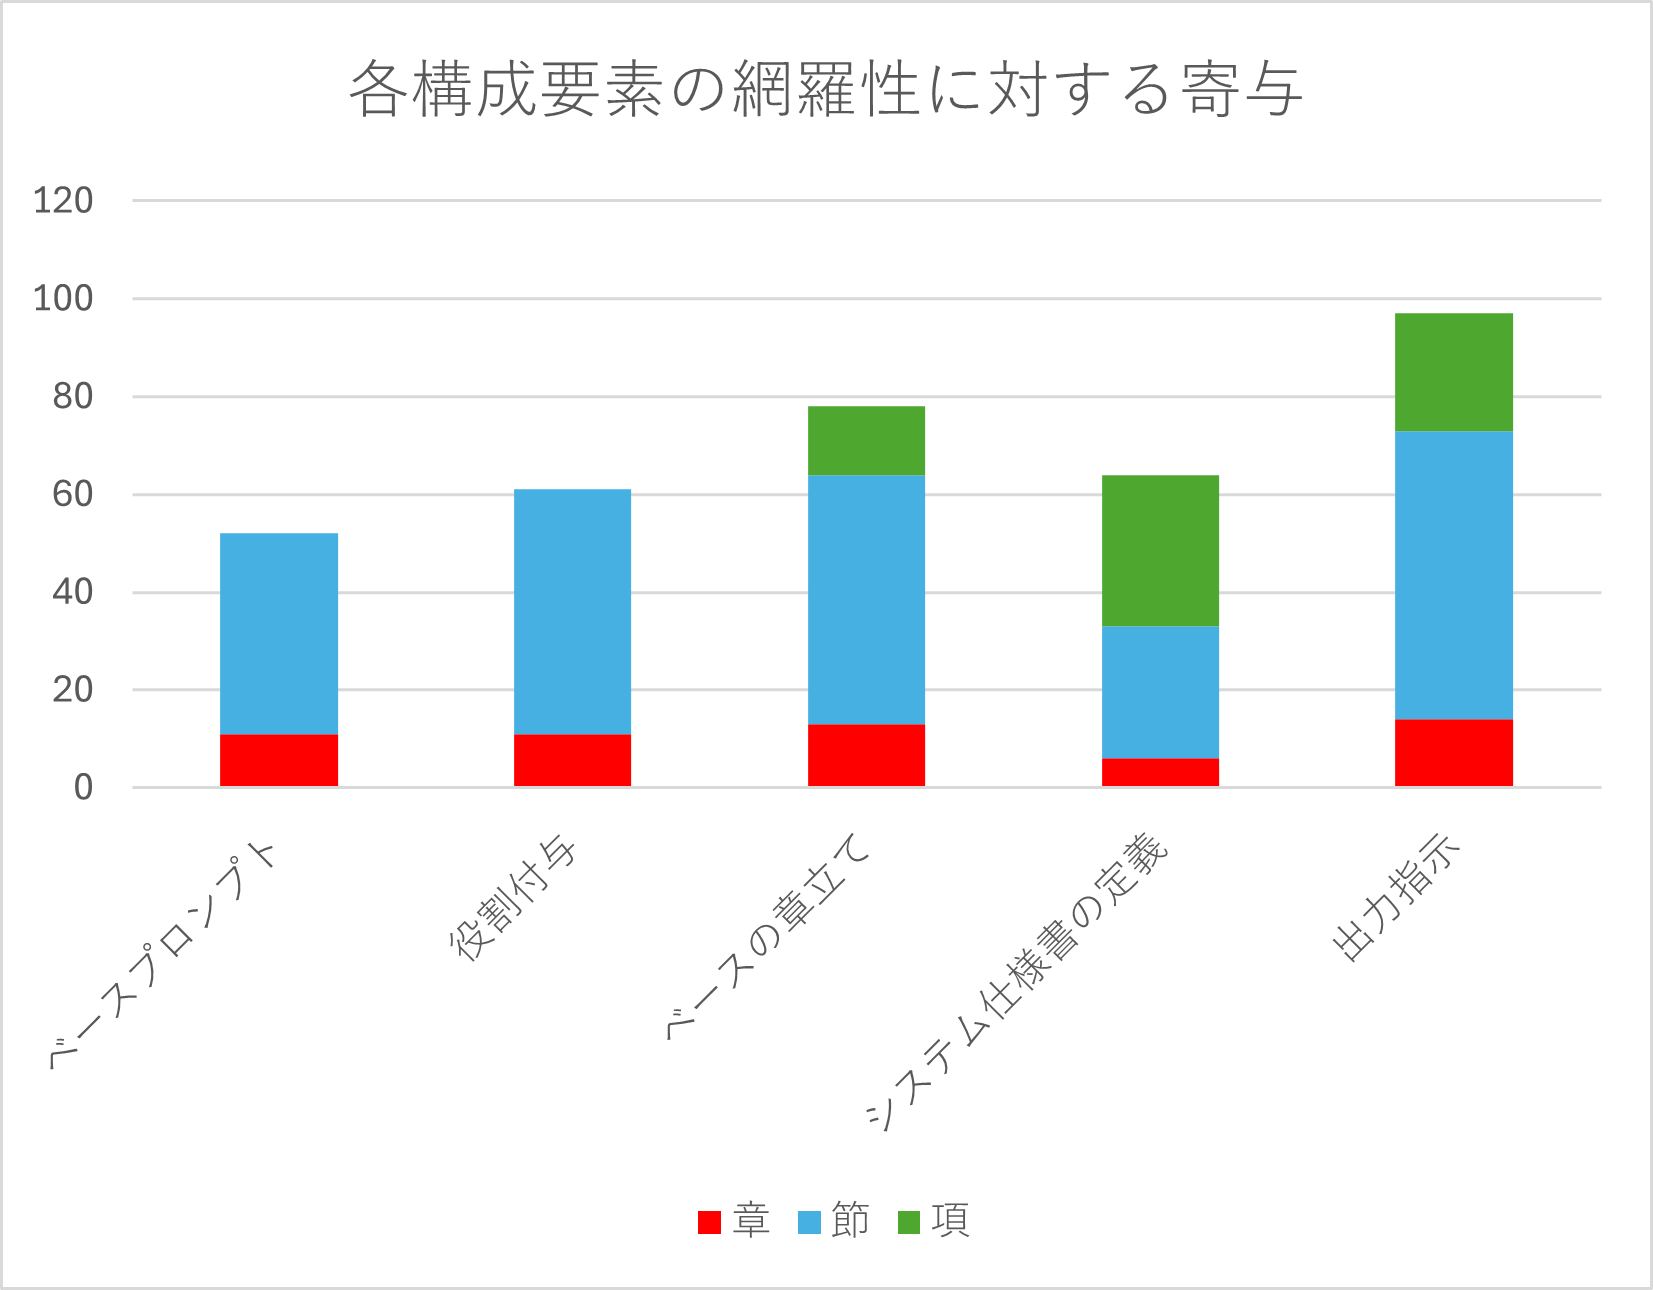
\includegraphics[width=0.8\textwidth]{images/網羅性.png}
%   \caption{各構成要素の網羅性に対する寄与}
%   \label{fig:coverage}
% \end{figure}

表\ref{tb:ieee}は、IEEE830がシステム仕様書の章立てに含むことを推奨する項目(図\ref{fig:ieee830}参照)と図\ref{fig:base_prompt_outline}、図\ref{fig:only_role_outline}、図\ref{fig:only_outline_outline}、図\ref{fig:only_definition_outline}、図\ref{fig:only_output_outline}に示した章立てを比較し、各プロンプトの構成要素がIEEE830がシステム仕様書の章立てに含むことを推奨する項目をどれだけ満たしているかを示した表である。
この表から、ベースプロンプト(図\ref{fig:base_prompt})による章立て(図\ref{fig:base_prompt_outline})は、IEEE830がシステム仕様書の章立てに含むことを推奨する項目を36項目中17項目満たしていることが分かる。
役割付与を追加したプロンプト(図\ref{fig:only_role})による章立て(図\ref{fig:only_role_outline})は、36項目中19項目満たしていることが分かる。
ベースの章立てテンプレートを追加したプロンプト(図\ref{fig:only_outline})による章立て(図\ref{fig:only_outline_outline})は、36項目中23項目満たしていることが分かる。
システム仕様書の定義を追加したプロンプト(図\ref{fig:only_definition})による章立て(図\ref{fig:only_definition_outline})は、36項目中11項目満たしていることが分かる。
出力指示(網羅性と自由度の指示)を追加したプロンプト(図\ref{fig:only_output})による章立て(図\ref{fig:only_output_outline})は、36項目中19項目満たしていることが分かる。

この結果からも、「システム仕様書の定義」は網羅性を低下させる要因であることが分かる。
一方で、「役割付与」、「ベースの章立て」、「出力指示」は網羅性の向上に寄与することが分かる。
特に、「ベースの章立て」は、網羅性に最も寄与することが分かる。

この結果から、網羅性の高い章立てを作成するためには、質の良い「ベースの章立て」を用意することが重要であると考察できる。
したがって、LLMとの対話を1回で終わらせるのではなく、1回目の生成結果の出力である章立てを、次回のプロンプトの「ベースの章立て」として再利用することで、章立てを段階的に洗練させる再帰的な手法が有効である可能性がある。


\begin{table}[tp]
  \centering
  \caption{IEEE830の章立てに含むことが推奨される項目と各プロンプト構成要素の対応}
  \label{tb:ieee}
%   \footnotesize
%   \renewcommand{\arraystretch}{1.2}
  \scriptsize
  \renewcommand{\arraystretch}{0.9}
  \setlength{\tabcolsep}{3pt}
  \begin{tabular}{|l|c|c|c|c|c|}
    \hline
    \textbf{仕様書の章立て項目} & \textbf{ベースプロンプトを追加} & \textbf{役割付与を追加} & \textbf{ベースの章立てを追加} & \textbf{仕様書の定義を追加} & \textbf{出力指示を追加} \\ \hline
    1. はじめに & & & & &〇 \\ \hline
    \forceindent1.1 本書の目的 & & &〇 & &〇 \\ \hline
    \forceindent1.2 対象範囲 &〇 & 〇& 〇& &〇 \\ \hline
    \forceindent1.3 用語定義・略語 &〇 & 〇& 〇& 〇&〇 \\ \hline
    \forceindent1.4 本書の構成 & & & & & \\ \hline
    2. システム概要 &〇 & 〇& 〇& 〇&〇 \\ \hline
    \forceindent2.1 システムの全体像 & 〇& 〇& 〇& 〇&〇 \\ \hline
    \forceindent\forceindent2.1.1 システム間インターフェース & & & & & \\ \hline
    \forceindent\forceindent2.1.2 画面インターフェース & & & & & \\ \hline
    \forceindent\forceindent2.1.3 ハードウェア構成 & & 〇& 〇& 〇& 〇\\ \hline
    \forceindent\forceindent2.1.4 ソフトウェア構成 & &〇 & 〇& & \\ \hline
    \forceindent\forceindent2.1.5 ネットワーク構成 &〇 &〇 &〇 &〇 & \\ \hline
    \forceindent\forceindent2.1.6 リソース制約 & & & & & \\ \hline
    \forceindent\forceindent2.1.7 運用環境 & & &〇 & & \\ \hline
    \forceindent\forceindent2.1.8 設置条件 & & & & & \\ \hline
    \forceindent2.2 システムの主な機能 &〇 &〇 &〇 &〇 &〇 \\ \hline
    \forceindent2.3 想定利用者 & & & & &〇 \\ \hline
    \forceindent2.4 制約事項 & 〇&〇 &〇 & & 〇\\ \hline
    \forceindent2.5 前提条件および依存関係 &〇 &〇 &〇 & & \\ \hline
    \forceindent2.6 将来対応事項 & & & & & 〇\\ \hline
    3. 詳細要件 & & &〇 & 〇&〇 \\ \hline
    \forceindent3.1 外部インターフェース仕様 &〇 &〇 &〇 & & \\ \hline
    \forceindent3.2 機能要件 &〇 &〇 &〇 &〇 &〇 \\ \hline
    \forceindent3.3 性能要件 &〇 &〇 &〇 &〇 &〇 \\ \hline
    \forceindent3.4 データベース要件 & & &〇 & & \\ \hline
    \forceindent3.5 設計上の制約事項 & & & & &〇 \\ \hline
    \forceindent3.6 システム品質特性 & & & & & \\ \hline
    \forceindent\forceindent3.6.1 信頼性 & & &〇 & & \\ \hline
    \forceindent\forceindent3.6.2 可用性 &〇 &〇 &〇 & &〇 \\ \hline
    \forceindent\forceindent3.6.3 セキュリティ &〇 &〇 &〇 &〇 &〇 \\ \hline
    \forceindent\forceindent3.6.4 保守性 & &〇 &〇 & & \\ \hline
    \forceindent\forceindent3.6.5 移植性 &〇 &〇 &〇 & &〇 \\ \hline
    \forceindent3.7 その他の要件 &〇 &〇 &〇 & 〇&〇 \\ \hline
    4. 参考資料 &〇 &〇 & & & \\ \hline
    \forceindent4.1 索引 & & & & & \\ \hline
    \forceindent4.2 付録 &〇 & & & & \\ \hline
    \textbf{合計} & \textbf{17}& \textbf{19}& \textbf{23}& \textbf{11}& \textbf{19}\\ \hline
  \end{tabular}
\end{table}




\iffalse
提案するプロンプトが高い評価を得た要因として、「ベース章立てテンプレート」と「記述の粒度に関する制約」の2点が大きく寄与していると考えられる。

まず、章立てテンプレートの提示は、「構造的整合性」の点数安定化に貢献した。
実験結果において、手法C(提案プロンプト)はBMPで3.8点、クラウドで3.7点と安定した点数を記録している。
これは、テンプレートという「型」があることで、章・節・項の包含関係が破綻することなく、論理的な構造が保たれたためである。

次に、「画面レイアウトと操作フローのみを含める」といった記述粒度の制約は、「可読性」と「適合性」の向上に寄与した。
自由プロンプト(手法B(自由プロンプト))のBMPの結果に見られるような「冗長すぎる」という評価を回避し、
開発の初期段階(概略設計)として適切な粒度に情報を絞り込む効果があったと考えられる。
これにより、プログラマやテスト担当者にとって「読みやすく、かつ必要な情報が含まれている」バランスの良い章立てが生成された。
\fi

\iffalse
本研究では、提案するプロンプトの各構成要素(「ベース章立てテンプレート」や「システム仕様書の定義」など)が生成結果に与える影響を確認するため、
一部の要素を削除したプロンプトを用いた追加実験を行った。
その結果、特定の要素を削除しても、生成される章立ての構造や内容に劇的な劣化が見られないケースが確認された。
これは、使用したLLM(GPT-5.2)が高い推論能力を持ち、プロンプトに明示的な指示がなくとも、文脈からシステム仕様書として必要な要素を自動的に補完したためと考えられる。

しかし、この事実は提案するプロンプトの各要素が不要であることを意味しない。
自由プロンプト(手法B(自由プロンプト))を用いた実験結果において、被験者Cの結果は「詳細すぎる(冗長)」となり、被験者Dの結果は「非常に高品質」となるなど、出力品質に大きなばらつきが見られたことを想起すべきである。
このばらつきは、制約のない状態でのLLMの生成が、入力されたわずかなニュアンスや確率的な揺らぎに大きく左右される「運任せ」の側面を持つことを示している。

この観点から、提案するプロンプトに含まれる「ベース章立てテンプレート」や「記述粒度の制約」といった要素は、常に最高点を目指すための「魔法」ではなく、
LLMが過剰に詳細化したり、逆に必要な項目を見落としたりするのを防ぐ「安全装置(ガードレール)」として機能していると結論付けられる。
追加実験で大きな差が出なかったのは、たまたまLLMが適切な方向へ補完を行ったためであるが、
手法C(提案プロンプト)全体として安定した高評価(特に構造的整合性や可読性において)が得られている事実は、
このガードレールが機能し、どのようなシステムや状況であっても一定水準以上の品質を担保し続けていることの証左である。
\fi

\subsection{手法B(自由プロンプト)で被験者が作成したプロンプトとの比較}
\subsubsection{BMP画像分割アプリの章立て作成において、被験者Cが作成したプロンプトとの比較}
図\ref{fig:c_prompt}に、BMP画像分割アプリにおいて手法B(自由プロンプト)を用いた被験者Cが用いたプロンプトを示す。
被験者CはLLMと4回の対話を行い、章立ての作成を行った。

\begin{figure}[tp]
\begin{tcolorbox}[
  colback=white,
  colframe=green!35!black,
  fonttitle=\bfseries,
]
\footnotesize
\ttfamily
\fontsize{7}{8}\selectfont
\begin{verbatim}
1回目の対話時のプロンプト----------------------------------------------------------
まず章立てテンプレートを送ります
(中略: ベースの章立てテンプレート)

2回目の対話時のプロンプト----------------------------------------------------------
- システム名：BMP画像分割アプリ
- 概要：指定されたBMP画像ファイルを指定された数に分割する。
このシステムについての章立てを行ってほしい
足りない章や節は追加し、いらない章や節は削除してください

3回目の対話時のプロンプト----------------------------------------------------------
章立てだけにしてください。小節などにできそうなものは小節にしてください

4回目の対話時のプロンプト----------------------------------------------------------
現在は章と節のみになっています。小節はありませんか？また小節にできる節はありませんか？
\end{verbatim}
\end{tcolorbox}
\par\vspace{-10pt}
\captionof{figure}{被験者Cが手法BでBMP画像分割アプリの章立て生成に対して用いたプロンプト}
\label{fig:c_prompt}
\end{figure}

被験者Cは、「小節はありませんか？」「小節などにできそうなものは小節に」といった指示を繰り返し行い、章立ての詳細化を図った。
その結果、網羅性は高まったものの、評価者からは「冗長」「粒度が細かすぎる」との指摘を受け、拡張性の低下(2.8点)を招いた。
これは、LLMに対して「詳細化」のみを強く求めた結果、仕様書全体のバランスが崩れ、過剰な階層構造が生成されたためである(図\ref{fig:B_chapter_structure_of_bmp_app}参照)。
提案プロンプトでは、テンプレートと制約によって章立ての詳細化を制御しており、このような過剰な細分化を防ぐ効果があったことが確認できる。

\subsubsection{クラウド型電子契約サービスの章立て作成において、被験者Dが作成したプロンプトとの比較}
図\ref{fig:d_prompt}に、クラウド型電子契約サービスにおいて手法B(自由プロンプト)を用いた被験者Dのプロンプトを示す。

\begin{figure}[tp]
\begin{tcolorbox}[
  colback=white,
  colframe=green!35!black,
  fonttitle=\bfseries,
]
\footnotesize
\ttfamily
\fontsize{8}{9}\selectfont
\begin{verbatim}
クラウド型電子契約サービスの仕様書を作成しようとしています。章立てテンプレートを参考に、仕様書の目次を作成してください

システム名：クラウド型電子契約サービス
概要：PDF技術を活かした電子契約／ワークフロー、それらに付随する文書管理、及びユーザー管理機能を持つクラウドサービス

【ベース章立てテンプレート(参考)】
(中略: ベースの章立てテンプレート)

※ベース章立てはあくまで参考です。必要に応じて章の追加・削除・順序変更を行って、漏れなく体系的な章立てを作成してください。
\end{verbatim}
\end{tcolorbox}
\captionof{figure}{被験者Dが手法Bでクラウド型電子契約サービスの章立て作成に対して用いたプロンプト}
\label{fig:d_prompt}
\end{figure}

被験者Dは、LLMにシンプルな章立て作成指示とベースの章立てのみを与えた。
電子契約サービスのような複雑で一般的なドメイン知識が豊富な分野においては、この「シンプルな指示」によって、
粒度の適切さ(4.8点)や独自性(4.6点)の高い、非常に優れた章立てが生成された(表\ref{tb:cloud_detailed_evaluation_results_B}参照)。
提案プロンプトは、システム仕様書の定義内の明示的な制約が逆に作用し、LLMが持つ豊富な知識の活用を一部阻害した可能性があり、粒度の適切さが手法C(提案プロンプト)で3.4点と低かった要因であると考える。
このことから、対象システムが一般的で多くの既存事例が存在するシステムであり、かつ複雑な機能を持つ場合は、
提案プロンプトの制約を一部緩和するか、指示を簡潔にすることが有効である可能性があると考察する。

\section{対象とするシステムの複雑さによる影響}
本実験では、単純な機能を持つ「BMP画像分割アプリ」と、複雑な機能を持つ「クラウド型電子契約サービス」という2つのシステムを実験に用いた。
システムの複雑さが異なっても、提案プロンプトは一定の有用性を示したが、その挙動には差異が見られた。


図\ref{fig:acomparison}に、手法A(手動作成)のBMP画像分割アプリとクラウド型電子契約サービスの評価結果(表\ref{tb:bmp},表\ref{tb:cloud}参照)の比較を示す。
\begin{figure}[tp]
    \centering
    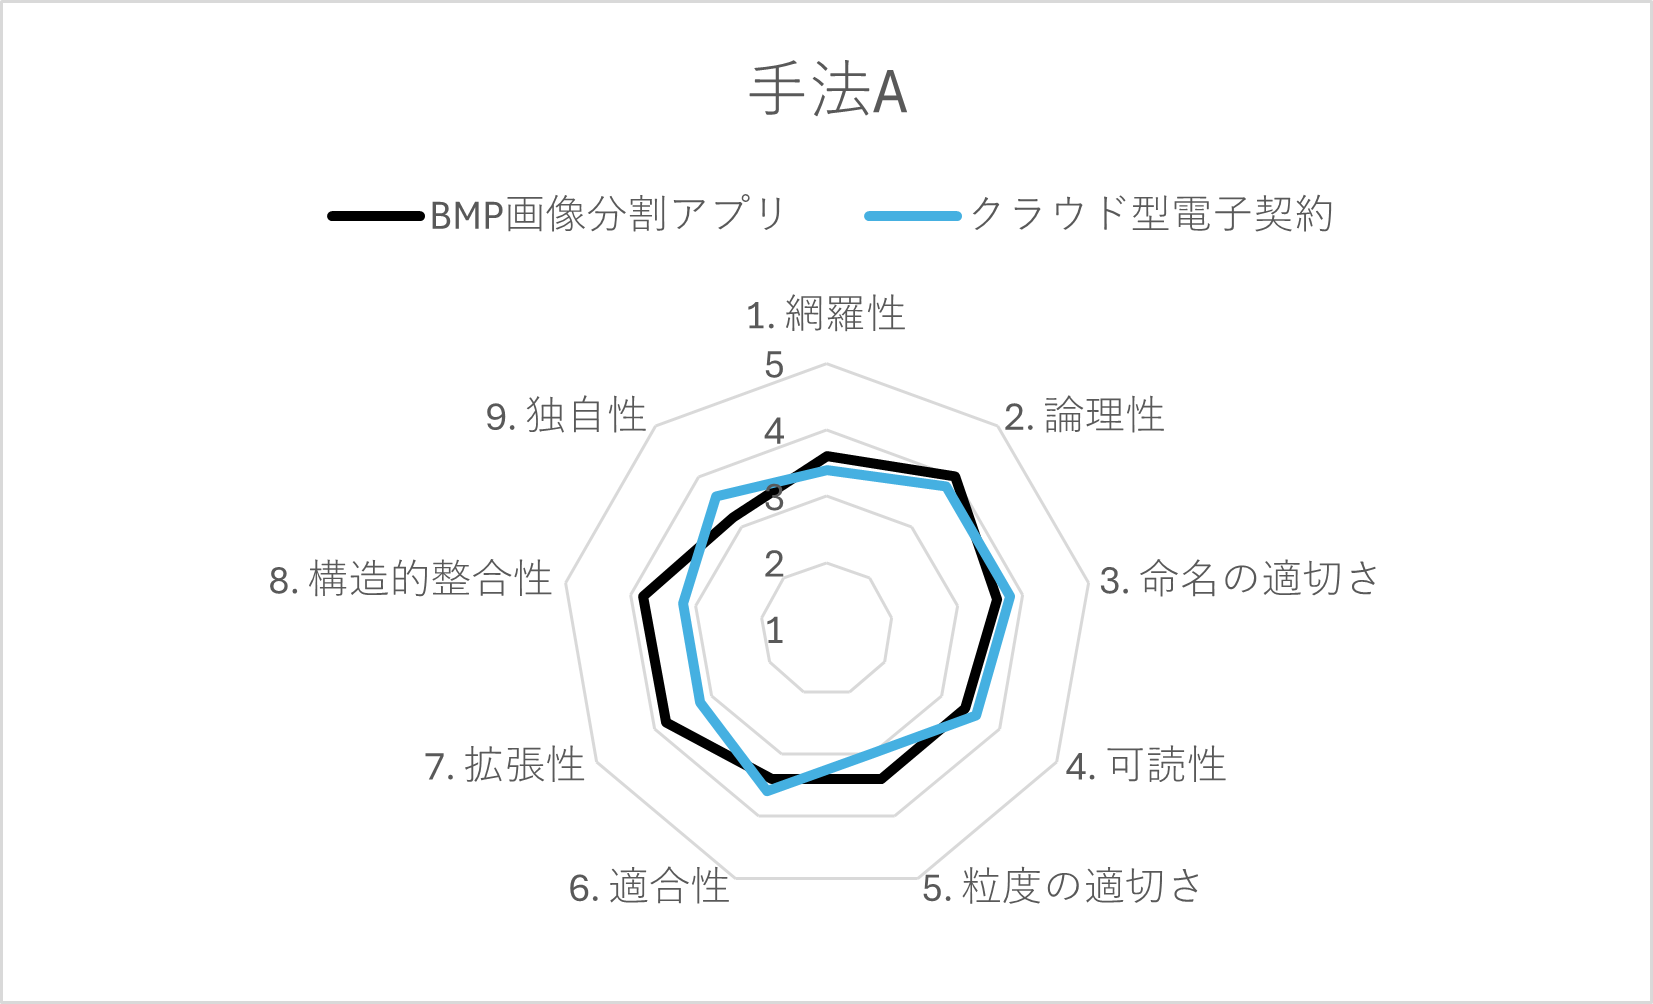
\includegraphics[width=0.8\textwidth]{images/手法Aばらつき.png}
    \caption{手法A(手動作成)の評価結果のばらつき}
    \label{fig:acomparison}
\end{figure}

図\ref{fig:bcomparison}に、手法B(自由プロンプト)のBMP画像分割アプリとクラウド型電子契約サービスの評価結果(表\ref{tb:bmp},表\ref{tb:cloud}参照)の比較を示す。
\begin{figure}[tp]
    \centering
    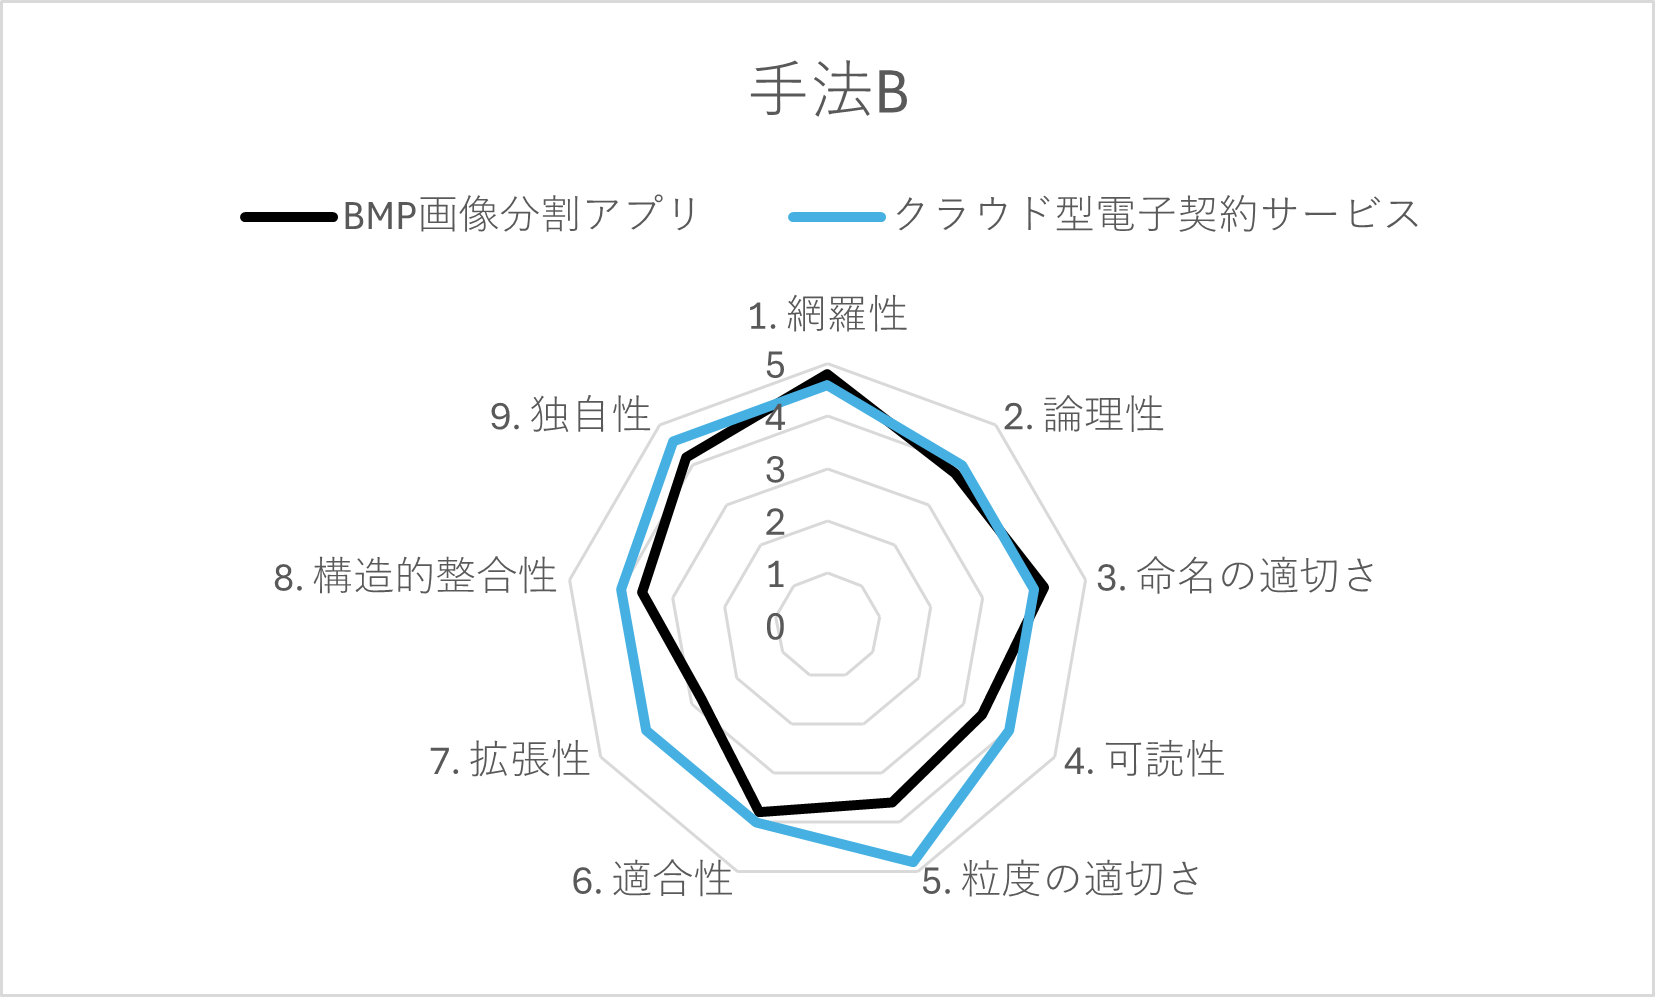
\includegraphics[width=0.8\textwidth]{images/手法Bばらつき.png}
    \caption{手法B(自由プロンプト)の評価結果のばらつき}
    \label{fig:bcomparison}
\end{figure}

図\ref{fig:ccomparison}に、手法C(提案プロンプト)のBMP画像分割アプリとクラウド型電子契約サービスの評価結果(表\ref{tb:bmp},表\ref{tb:cloud}参照)の比較を示す。
\begin{figure}[tp]
    \centering
    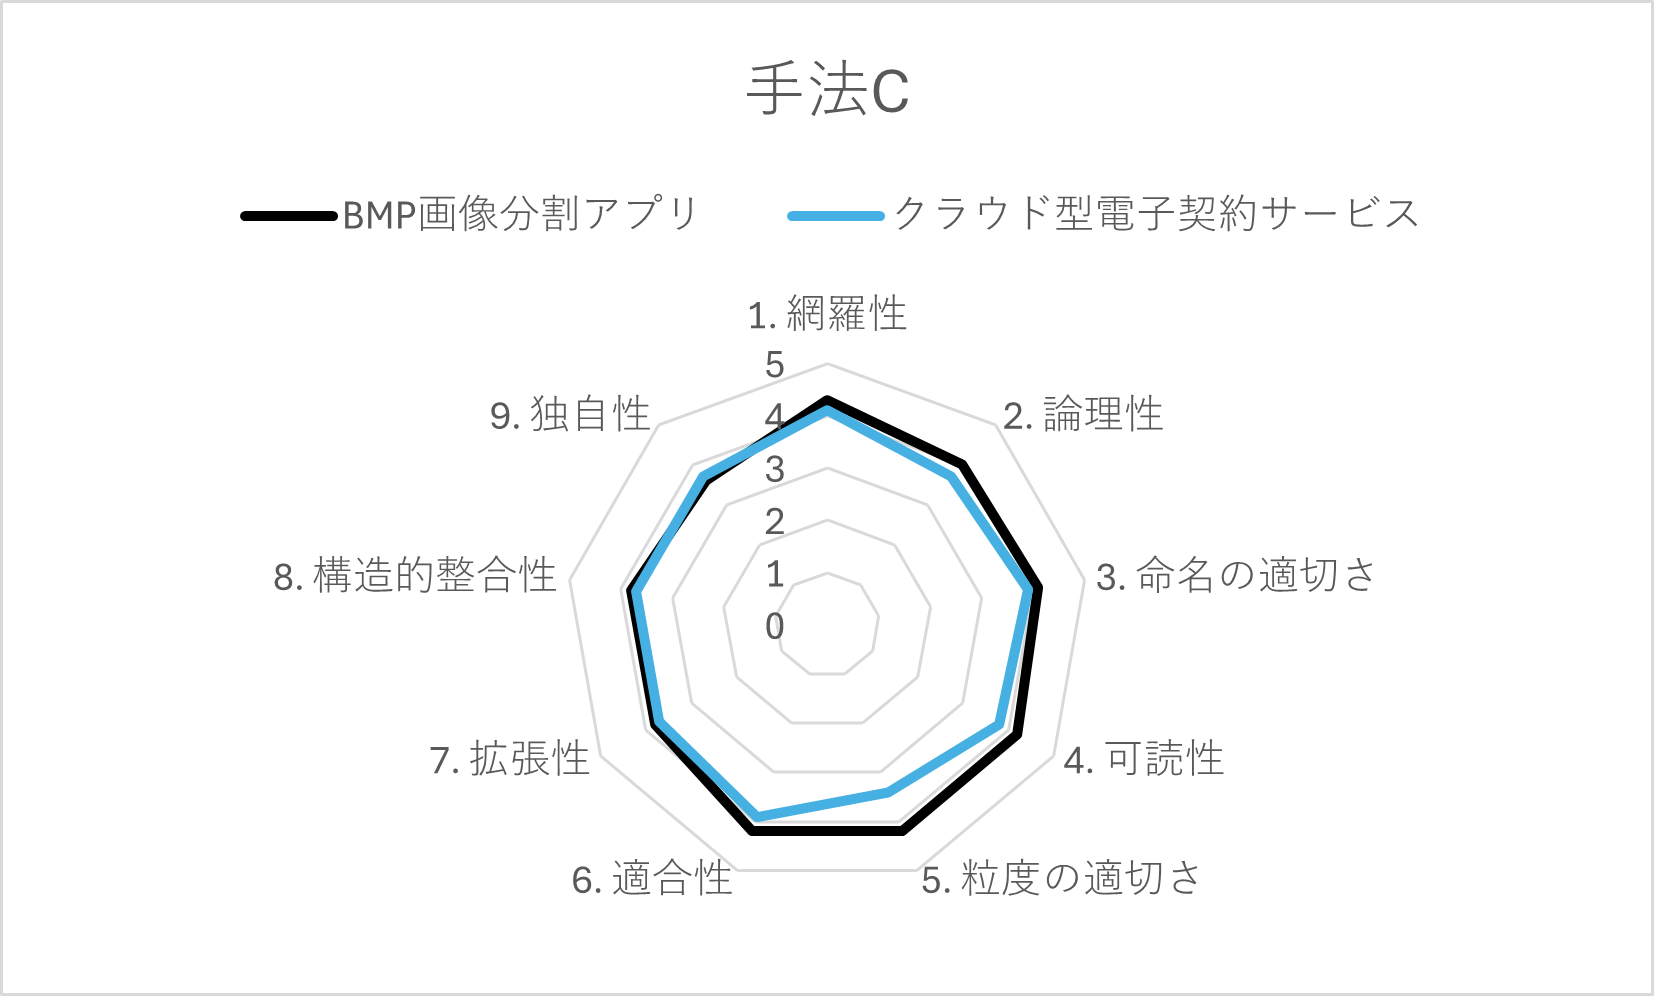
\includegraphics[width=0.8\textwidth]{images/手法Cばらつき.png}
    \caption{手法C(提案プロンプト)の評価結果のばらつき}
    \label{fig:ccomparison}
\end{figure}

図\ref{fig:acomparison}、図\ref{fig:bcomparison}、図\ref{fig:ccomparison}を比較すると、手法A、Bに比べ、手法Cは対象システムによる評価結果のばらつきが小さいことがわかる。

この結果は、手法B(自由プロンプト)は高い品質の章立てを出す可能性がある一方で、BMP画像分割アプリのような単純なシステムに対しては、冗長な構成が、拡張性、可読性の低下といったリスクにつながることを示している。
手法C(提案プロンプト)は、独自性や粒度の適切さでは自由プロンプトの最良ケースに劣るものの、対象とするシステムの複雑さが変わることによる章立ての品質のばらつきを抑えることができる点に特長があると言える。



また、単純なシステムであるBMP画像分割アプリにおいては、提案プロンプトは極めて有効に機能した。
手法C(提案プロンプト)の結果(表\ref{tb:detailed_evaluation_results_C}参照)は、網羅性4.4点、可読性4.4点、適合性4.4点と非常に高く、テンプレートが、小規模システムの全体像をカバーするのに十分であったことを示している。

一方、複雑なシステムであるクラウド型電子契約サービスにおいては、提案プロンプトの評価は総じて良好であったものの、項目によっては自由プロンプト(手法B(自由プロンプト))に劣る結果も見られた。

まず、提案プロンプトを用いた被験者間の評価結果のばらつきについて、被験者A(手法C(提案プロンプト))の粒度の適切さ(表\ref{tb:cloud_detailed_evaluation_results_C}参照)は2.8点と低く、被験者C(手法C(提案プロンプト))は4.0点であった。
同じプロンプトを使用しても、出力される粒度の適切さにばらつきが生じたことは、LLMの確率的な生成特性によるものと考えられる。

また、複雑なシステムでは、システム全体を俯瞰するだけでなく、個々の機能(ワークフロー図、排他制御など)について深い記述が求められるため、
手法C(提案プロンプト)のベースの章立てや制約では、LLMの生成能力を十分に引き出せない場合があると考えられる。

結論として、提案プロンプトはシステムの複雑さに関わらず「一定品質の保証」には寄与する。
しかし、複雑なシステムにおいて「高品質」かつ「高詳細」な章立てを目指す場合には、機能ごとに分割して生成する、あるいはChain-of-thoughtプロンプト\cite{chainofthought}を用いて章立てを段階的に出力していくといった、プロンプトエンジニアリングの更なる工夫が必要となる。

\section{まとめ}

本章の分析から、提案プロンプトについて、以下の3点が明らかになった。

\subsection{提案プロンプトの特長}
\label{sec:features_of_proposed_prompt}
提案プロンプトの最大の特長は、対象とするシステムの特性の違いによる章立ての品質のばらつきを抑制できる点である。

手法A(手動作成)との比較では、単純なシステム(BMP画像分割アプリ)における「項目の抜け漏れ」や、複雑なシステム(クラウド型電子契約サービス)における「ドメイン知識不足による独自性の欠如」といった、システムの特性ごとに生じやすい課題を、
役割付与とベース章立てテンプレート、出力指示(網羅性と自由度の指示)によって共通して補完できることを示した(表\ref{tb:bmp}、表\ref{tb:cloud}参照)。
特に、網羅性においてBMP画像分割アプリで手法A(手動作成)(3.6点)に対し、手法C(提案プロンプト)(4.3点)、
独自性においてクラウド型電子契約サービスで手法A(手動作成)(2.8点)に対し、手法C(提案プロンプト)(3.7点)と、システムの特性に関わらず改善した(表\ref{tb:bmp}、表\ref{tb:cloud}参照)。

手法B(自由プロンプト)との比較では、自由プロンプトがシステムの特性によって品質が大きく変動する(BMP: 34.2点、クラウド: 38.0点、差3.8点)のに対し、
提案プロンプトは対象システムが異なっても一定水準の品質(BMP: 36.2点、クラウド: 33.9点、差2.3点)であることを確認した(図\ref{fig:bcomparison}、図\ref{fig:ccomparison})。
自由プロンプトはクラウドサービスのような複雑なシステムでは高品質(粒度の適切さ4.8点、独自性4.6点)を達成する一方、単純なシステムでは過剰な詳細化などの問題が生じたが、
提案プロンプトは自由プロンプトと比較して、システムの特性に左右されにくいと言える。

\subsection{提案プロンプトの限界}
\label{sec:limitations_of_proposed_prompt}

提案プロンプトには、以下のトレードオフが存在することが明らかになった。

\begin{itemize}
    \item \textbf{網羅性と適合性}: システム仕様書の定義による制約は、適合性を高める(BMP: 4.2点、クラウド: 3.9点)代わりに、
    網羅性や独自性が低下する。これが、手法B(自由プロンプト)の最良ケースに劣る要因となっている。
    
    \item \textbf{網羅性と粒度の適切さ}: 出力指示(網羅性と自由度の指示)は網羅性を高める一方、
    階層が深くなりすぎて粒度の適切さの評価を下げる可能性がある。
    
    \item \textbf{テンプレートの制約}: ベース章立てテンプレートは命名の適切さを向上させるが、
    テンプレートに含まれない項目が生成されにくくなる可能性がある。
\end{itemize}

% これらのトレードオフは、提案するプロンプトが「システムの特性に依存しない汎用的な品質保証」を実現するための必然的な帰結である。
% 自由プロンプトが、対象システムに対するLLMの学習データ量やシステムとLLMの相性に依存して品質が大きく変動する「不確実性」を持つのに対し、提案するプロンプトは、あらゆるシステムに対して一定水準以上の網羅性と論理的構造を担保する「堅牢性」を備えている。
% すなわち、これは単なる妥協ではなく、実務において最も重要視される「品質の予測可能性と安定性」を、対象システムの規模や複雑さに関わらず提供できるという、本手法の核心的な価値を示している。

% これらのトレードオフは、提案するプロンプトが「品質の安定化」を優先した設計であることに起因する。
% すなわち、最高点を目指すのではなく、最低点を引き上げることに重点を置いた結果、
% 自由プロンプトの最良ケースには及ばないものの、安定した品質を実現している。

\subsection{提案プロンプトの適用場面の使い分け}

\ref{sec:features_of_proposed_prompt}節と\ref{sec:limitations_of_proposed_prompt}節の分析から、提案プロンプトの適用場面について、以下の示唆が得られる。

\textbf{提案プロンプトが特に有効な場面}
\begin{itemize}
    \item 仕様書作成の経験が浅いメンバーが作成する場合
    \item 小〜中規模のシステムで、標準的な構成が求められる場合
    \item 短時間で一定品質の章立てを確実に得たい場合
\end{itemize}

% \textbf{自由プロンプトとの併用を検討すべき場面}
\textbf{提案プロンプトの制約を緩める必要がある場面}
\begin{itemize}
    \item 複雑なシステムで、独自性が求められる場合
    \item LLMが豊富な知識を持つドメインのシステムで、その知識を最大限活用したい場合
    \item システム仕様書作成の経験と知識が豊富な作成者が、最高品質を目指す場合
\end{itemize}

このような使い分けにより、提案プロンプトの「品質の安定化」という強みを活かしつつ、
必要に応じて自由度を高めることで、より効果的な章立て生成が可能になると考える。

システムの複雑さに関する考察からは、以下の知見を得た。
単純なシステム(BMP画像分割アプリ)においては、提案プロンプトは極めて有効に機能し、網羅性4.4点、可読性4.4点、適合性4.4点と非常に高い評価を得た。
これは、テンプレートが小規模システムの全体像をカバーするのに十分であったことを示している。

一方、複雑なシステム(クラウド型電子契約サービス)においては、提案プロンプトは総じて良好な評価を得たものの、
同一のプロンプトを使用しているにも関わらず、生成された章立ての「粒度の適切さ」において評価にばらつきが生じる結果となった(被験者A: 2.8点、被験者C: 4.0点)。
これは、同じ制約とテンプレートを与えても、複雑なシステムにおいてはLLMの出力の品質が生じやすく、完全に品質を均一化することの難しさを示唆している。
複雑なドメインでは、個々の機能について深い記述が求められるため、
画一的なテンプレートや制約だけでは、LLMの生成能力を十分に引き出せない場合がある。

したがって、複雑なシステムにおいては、提案プロンプトをベースとしつつ、
Chain-of-thoughtプロンプト\cite{chainofthought}を取り入れ、機能ごとに分割して生成する、あるいは、
網羅的な章立てを生成してから、章立てテンプレートに沿って整形していくといった、
段階的なアプローチが有効である可能性があると結論付ける。


% おわりに
\chapter{おわりに}\label{cha:Conclusion}

本研究では、対象とするシステムの特性に合わせた、システム仕様書の章立てを自動生成することを目的として、LLMを用いたシステム仕様書章立て作成のためのプロンプトを提案した。
提案プロンプトは、プロンプトエンジニアリングの技術であるPersona Pattern、One-shot Prompting、Context-Manager Patternを組み合わせることで、標準的な章立ての維持と、対象システムの特性を反映した章立ての拡張の両立を目指して設計した。
提案プロンプトの5つの構成要素を、以下に示す。
\begin{itemize}
    \item 役割付与
    \item ベースの章立て
    \item 開発するシステム情報
    \item システム仕様書の定義
    \item 出力指示
\end{itemize}

提案プロンプトの有用性を確かめるために、BMP画像分割アプリとクラウド型電子契約サービスという2つの異なるシステムを対象として、LLMを用いずに章立てを作成する手法、LLMに自由なプロンプトを与えて章立てを作成する手法、LLMに本研究で提案したプロンプトを与えて章立てを作成する手法の3つの手法で章立てを作成し、その章立ての品質を専門家5人が評価した。
結果として、提案プロンプトは、LLMを用いずに章立てを作成する手法と比較して、章立ての作成に有用であると言えた。
また、提案プロンプトを用いた手法は、LLMに自由なプロンプトを与えた手法と比較して、BMP画像分割アプリのような機能が少ない単純なシステムにおいては、提案プロンプトは有用であると言えた。
一方で、クラウド型電子契約サービスのような機能が多い複雑なシステムにおいては、粒度の適切さや独自性の観点においては、有用であるとは言えなかった。
これは、提案プロンプトに含まれる、章立て生成に対する制約が、複雑なシステムにおいてはLLMの知識活用を阻害し、網羅性が低下したためだと考える。

以下に今後の課題を示す。

\begin{itemize}
    \item より多様なシステムでの提案プロンプトの適用実験と評価\\
    本研究においては、2種類のシステムを対象として実験を行ったが、今後はより多様なシステムを対象として実験を行い、提案プロンプトの有用性と課題を確かめる必要がある。
    \item Chain-of-Thoughtの導入によるシステム仕様書章立て生成プロンプトの改善\\
    本研究の評価実験の結果から、複雑なシステムにおいては、一度に最終的な章立てを生成するのではなく、まず、網羅性を高めることに注力するべきであるという知見を得た。
    そのため、プロンプトにプロンプトエンジニアリング技術の1つであるChain-of-Thoughtを導入し、まずは制約を緩めた状態でシステムに必要な要件や機能を網羅的に列挙させ、その後に、ベースの章立てテンプレートや、システム仕様書の定義に基づいて、章立てを構造化、整形していくというアプローチが有効であると考える。
\end{itemize}

% 本研究では、大規模言語モデル（LLM）を用いて、対象システムの規模や複雑さに関わらず、網羅的かつ論理的なシステム仕様書の章立てを自動生成する手法を提案した。
% 提案手法は、プロンプトエンジニアリングの技術（Persona Pattern, One-shot Prompting, Context-Manager Pattern）を応用し、「役割付与」「ベース章立て」「システム仕様書の定義」「出力指示」といった構成要素を組み合わせることで、標準的な構造の維持と、対象システムの特性に応じた柔軟な拡張の両立を目指して設計された。

% 提案手法の有効性を検証するため、規模の異なる2つのシステム（BMP画像分割アプリ、クラウド型電子契約サービス）を対象に、専門家による比較評価実験を行った。
% 比較対象として、「手動作成」および「自由プロンプトによる生成」を用い、生成された章立ての品質を多角的に評価した。

% 実験の結果、提案手法は手動作成と比較して、「網羅性」「可読性」「構造的整合性」などの多くの項目で高い評価を得た。
% 特に、経験の浅い作成者が陥りやすい章立ての抜け漏れや、階層構造の不整合といった問題を解消し、実用的な品質の章立てを安定して生成できることが示された。
% また、自由プロンプトを用いた手法との比較においては、提案手法の特性として「安定性」と「品質の均一化」が確認された。
% 自由プロンプトは、LLMの知識を最大限に引き出すことで高い網羅性や独自性を発揮する場合がある一方、プロンプト作成者のスキルや偶然性に左右されやすく、冗長な構成や整合性の欠如といったリスクも伴うことが明らかになった。
% これに対し、提案手法は、明示的な制約とテンプレートを与えることで過度な生成を抑制し、評価者から「最も整理されている」「バランスが良い」と評される、実務に適した章立てを安定して出力することに成功した。

% 一方で、課題も明らかになった。
% クラウド型電子契約サービスのような複雑かつ大規模なシステムにおいては、提案手法の制約がLLMの知識活用を一部阻害し、自由プロンプトに比べて網羅性や独自性が低下する傾向が見られた。
% これは、作成者のドメイン知識不足を補うという点においては一定の効果があったものの、大規模システム特有の数多の要件を洗い出し、かつそれを厳密な構造に収めるという高度なタスクにおいては、現在のプロンプト構成では制約が強すぎた可能性がある。

% 今後の課題として、以下の2点が挙げられる。

% 第一に、より多様なシステムに対する適用と評価である。
% 本研究では2種類のシステムのみを対象としたが、さらに多様なドメインや規模のシステムに対して実験を行い、提案手法の汎用性と限界をより詳細に検証する必要がある。

% 第二に、Chain-of-Thought (CoT) の導入によるプロンプトの改善である。
% 複雑なシステムにおいては、一度に最終的な章立てを出力させようとするのではなく、思考プロセスを段階的に踏ませるアプローチが有効であると考えられる。
% 具体的には、まず制約を緩めた状態でシステムに必要な要件や機能を網羅的に列挙させ（発散）、その後にベース章立てや定義に基づいて構造化・整形を行う（収束）という、2段階の生成プロセスを導入することで、網羅性と構造的整合性の両立をより高いレベルで実現できると期待される。


% \section{研究の総括}
% 本研究により得られた成果は以下の通りである。

% 第一に、提案するプロンプトを用いることで、経験の浅い作成者であっても、実用的な品質の章立てを生成できることを確認した。
% 評価実験の結果、提案手法（手法C）は、手動作成（手法A）と比較して、「網羅性」「可読性」「適合性」「構造的整合性」の多くの項目で高い評価を得た。
% 特に、手動作成で見られた「章立ての抜け漏れ」や「階層構造の不整合」といった問題を解消し、安定して高品質な章立てを生成できることが示された。

% 第二に、提案手法は、自由なプロンプト（手法B）と比較して、品質のばらつきを抑制し、バランスの取れた章立てを生成できることを明らかにした。
% 自由なプロンプトを用いた場合、LLMの知識を最大限に引き出すことで、特定のケース（大規模なクラウドサービス等）において高い詳細度や独自性を発揮する可能性がある一方で、冗長な構成や論理的な不整合が生じるリスクも確認された。
% これに対し、提案手法は、明示的な制約とテンプレートを与えることで、過度な生成を抑制し、評価者から「最も整理されている」「バランスが良い」と評される実務に適した章立てを安定して出力することに成功した。

% 以上の結果から、本研究の目的である「標準化とドメイン適応の両立」を実現し、システム仕様書作成の効率化と品質向上に寄与する手法を確立したと言える。

%%
% 謝辞
%
\acknowledgment

本論文の執筆にあたり、親身にご指導、ご教授していただきました、宮崎大学工学部工学科情報通信工学プログラムの片山徹郎教授に、心より感謝申し上げます。

そして、株式会社スカイコムの皆様には、本研究にあたり、多くのアドバイスとご協力を賜りました。厚く御礼申し上げます。

また、本研究の遂行にあたり、片山徹郎研究室の皆様に大変お世話になりました。評価実験に参加してくださった皆様、長い時間をかけて論文の添削をしてくださった先輩方、差し入れをくださった先輩方、本当にありがとうございました。

さらに、同期の有馬君、原君、宮原君にも感謝申し上げます。研究だけでなくETロボコンも含め、長く苦楽を共にしました。貴方方の何事にも全力で取り組む姿勢に、何度も刺激を頂きました。ありがとうございました。

最後に、学生生活全般において、精神的、経済的に多大な支援をしてくれた家族に、深く感謝いたします。



%%
% 参考文献
%
%%
% 参考文献
%
\nocite{*}
\bibliography{paper} %hoge.bibから拡張子を外した名前
\bibliographystyle{junsrt} %参考文献出力スタイル
%%
% 付録
%
% \appendix{} % 付録は基本的に使わない

\end{document}
